\documentclass[pnumromarab,normalnum,abnttoc,times]{politex}
% ============================================================
%  Relatório Final — Projeto de Formatura I (PF1)
%  Classe: politex (POLI-USP).  Opções:
%   pnumromarab - romanos no pré-textual, arábicos no textual
%   normalnum   - numeração contínua de figuras/tabelas
%   abnttoc     - "p." nas páginas do sumário (ABNT)
%   times       - fonte Times New Roman
% ============================================================

% ========== Codificação e idioma ==========
\usepackage[utf8]{inputenc}
\usepackage[T1]{fontenc}
\usepackage[brazil]{babel}

% ========== Matemática ==========
\usepackage{amsmath,amssymb,amsthm}

% ========== Figuras e tabelas ==========
\usepackage{graphicx}
\usepackage{booktabs}
\usepackage{array}
\usepackage{multirow}
\usepackage{float}
\graphicspath{{figuras/}}

% ========== Cor e marcadores ==========
\usepackage{xcolor}

% ========== Referências bibliográficas (ABNT numérico) ==========
\usepackage[num]{abntex2cite}
\citebrackets{[}{]}

% ========== Hyperlinks ==========
%\usepackage[hidelinks]{hyperref}

% ========== Comandos auxiliares ==========
% Fonte da figura (linha inferior, conforme ABNT)
\newcommand{\fonte}[1]{{\footnotesize Fonte: #1}}
% Marcador de pendência (material a ser inserido pelas autoras)
\newcommand{\TODO}[1]{\textcolor{red}{\textbf{[A FAZER: #1]}}}

% ========== Opções do documento ==========
\titulo{Estratégias de controle distribuído para sistemas de armazenamento em baterias para regulação de tensão em redes de distribuição com alta penetração de geração fotovoltaica}

\autor{Ana Júlia de Morais Faria\\%
       Rafaela Sousa de Alencar Lacerda}

\orientador{Prof.\ Dr.\ Juan Carlos Cebrian}

\comentario{Relatório do Projeto de Formatura~I apresentado à Escola Politécnica da Universidade de São Paulo para conclusão do curso de Engenharia Elétrica.}

\local{São Paulo}
\data{2026}

\begin{document}

% ========== Capa e folhas de rosto ==========
\capa
\falsafolhaderosto
\folhaderosto

% ========== Resumo ==========
\begin{resumo}
A crescente penetração de geração fotovoltaica (FV) nas redes de distribuição 
de média tensão impõe desafios de regulação de tensão, sobretudo pela 
ocorrência de sobretensões nos períodos de maior irradiância. Este trabalho 
investiga uma estratégia de controle distribuído em duas camadas para 
Sistemas de Armazenamento de Energia em Baterias (BESS), com o objetivo de 
regular a tensão de forma autônoma e coordenada. Foi desenvolvido um ambiente 
de cossimulação acoplando Python e o software OpenDSS, sobre o qual se 
implementou um gerador de cenários pelo método de Monte Carlo aplicado à 
rede de teste IEEE~34 barras, contemplando onze níveis de penetração FV. A 
camada de controle primário baseia-se na curva volt-var normatizada pela 
ABNT~NBR~16149:2013, atuando localmente sobre a potência reativa dos 
inversores; a camada secundária emprega um algoritmo de consenso sobre a
potência ativa dos BESS, combinado a uma parcela de droop local, que ajusta a
potência ativa de cada BESS em função da tensão na barra de instalação. 
Os resultados preliminares 
mostram que o controle primário reduz de forma expressiva e previsível o
número de barras consumidoras em sobretensão, enquanto o controle secundário 
por consenso, na rede e configuração estudadas, não reduziu as violações 
remanescentes em barras consumidoras, em 
razão da concentração espacial dos BESS no alimentador. As conclusões 
delimitam as condições de eficácia de cada camada e orientam os próximos 
passos do projeto.
%
\\[3\baselineskip]
%
\textbf{Palavras-Chave} -- Controle distribuído, Sistemas de armazenamento de energia em baterias, Regulação de tensão, Geração fotovoltaica, Algoritmo de consenso.
\end{resumo}

% ========== Abstract ==========
\begin{abstract}
The increasing penetration of photovoltaic (PV) generation in medium-voltage 
distribution networks raises voltage regulation challenges, particularly 
overvoltage during peak irradiance hours. This work investigates a two-layer 
distributed control strategy for Battery Energy Storage Systems (BESS) aimed 
at regulating voltage autonomously and in a coordinated manner. A 
co-simulation environment coupling Python and the OpenDSS software was 
developed, on top of which a Monte Carlo scenario generator was implemented 
for the IEEE~34-bus test feeder, spanning eleven PV penetration levels. The 
primary control layer relies on the volt-var curve standardized by 
ABNT~NBR~16149:2013, acting locally on the reactive power of the inverters; 
the secondary layer employs a consensus algorithm on the active power of the
BESS, combined with a local droop term that adjusts each unit's active power
according to the voltage at its installation bus. The strategies were evaluated in a paired
manner over the same scenarios. Results show that primary control 
significantly and predictably reduces the number of consumer (load-connected) 
buses in overvoltage, whereas the consensus-based secondary control, for the 
studied network and configuration, did not reduce the remaining violations in 
consumer buses, 
owing to the spatial concentration of the BESS along the feeder. The 
conclusions delimit the effectiveness conditions of each layer and guide the next steps of the project.
%
\\[3\baselineskip]
%
\textbf{Keywords} -- Distributed control, Battery energy storage systems, Voltage regulation, Photovoltaic generation, Consensus algorithm.
\end{abstract}

% ========== Listas ==========
\listadefiguras
\listadetabelas

% ========== Lista de símbolos ==========
\begin{pretextualsection}{Lista de símbolos}
\begin{description}
  \item[$V_i$] Tensão na barra de instalação do recurso $i$ (p.u.)
  \item[$V_\text{ref}$] Tensão de referência do sistema ($1{,}0$~p.u.)
  \item[$P_\text{inst}$] Potência ativa instalada do recurso distribuído
  \item[$Q_\text{max}$] Potência reativa máxima do inversor ($0{,}4358\,P_\text{inst}$)
  \item[$x_i$] Variável de consenso aumentada do BESS $i$
  \item[$\Delta P_i,\ \Delta Q_i$] Correções de potência ativa e reativa do controle secundário
  \item[$L$] Matriz Laplaciana do grafo de comunicação ($L = D - A$)
  \item[$A,\ D$] Matrizes de adjacência e de grau do grafo
  \item[$\lambda_2$] Segundo menor autovalor de $L$ (conectividade algébrica)
  \item[$\gamma$] Peso do desvio de tensão na variável de consenso ($\gamma = 2{,}0$)
  \item[$\alpha$] Ganho do algoritmo de consenso ($\alpha = 0{,}15$)
  \item[$k_\text{droop}$] Ganho do droop de potência ativa ($\approx 14{,}3$~p.u.$^{-1}$)
  \item[$k_t$] Índice de claridade
  \item[$\eta$] Nível de penetração fotovoltaica
\end{description}

\vspace{0.5cm}
\noindent\textbf{Siglas} \\
ANEEL — Agência Nacional de Energia Elétrica; \
BESS — \emph{Battery Energy Storage System}; \
BT — Baixa tensão; \
FV — Fotovoltaico; \
GD — Geração distribuída; \
MT — Média tensão; \
RED — Recurso energético distribuído; \
SoC — \emph{State of Charge} (estado de carga); \
SONDA — Sistema de Organização Nacional de Dados Ambientais.
\end{pretextualsection}

% ========== Sumário ==========
\sumario

% ============================================================
%  PARTE TEXTUAL
% ============================================================
\chapter{Introdução}
\label{cap:introducao}

As redes elétricas de distribuição são tradicionalmente passivas, ou seja, 
a potência flui de forma unidirecional da geração para o consumo~\cite{grainger1994}. 
Nesse modelo, a qualidade da energia, em especial a regulação de tensão e o fator de potência, 
é assegurada pela robustez da geração centralizada, como hidrelétricas e termelétricas, 
pouco sensível a variações de curto prazo. A crescente integração de fontes de geração distribuída 
(GD), como os sistemas fotovoltaicos (FV), transformou essas redes em redes ativas, nas quais o 
fluxo de potência passa a ser bidirecional, determinado tanto pela geração quanto pela carga. 
Tal transformação impõe novos desafios à operação e ao controle, sobretudo no que tange à regulação 
de tensão.

A disseminação da GD criou demanda por Sistemas de Armazenamento de Energia em Baterias 
(\emph{Battery Energy Storage Systems} --- BESS), empregados para armazenar o excedente de energia 
em horários de baixa demanda e injetá-lo na rede nos horários de ponta. A eficácia desses sistemas, 
contudo, depende diretamente da estratégia de controle adotada. O controle centralizado, 
tradicionalmente utilizado, apresenta limitações de escalabilidade e robustez, pois exige infraestrutura 
de comunicação complexa e é suscetível a falhas em um único ponto de processamento. Em contrapartida, 
as estratégias de controle distribuído permitem que cada unidade BESS tome decisões com base em 
informações locais e na comunicação parcial com vizinhos imediatos~\cite{nabatirad2022}, aumentando a 
confiabilidade e facilitando a operação \emph{plug-and-play} de novos dispositivos.

Os conjuntos formados por GD e BESS favorecem um controle distribuído e automático da rede por meio dos 
inversores que conectam tanto os geradores fotovoltaicos quanto os BESS. Ao controlar a potência ativa e 
reativa injetada ou absorvida, é possível regular a tensão localmente. À medida que cresce o número de 
BESS autônomos e distribuídos, torna-se necessário coordená-los, de modo que operem de forma harmônica 
também em nível global, sem deteriorar os perfis de tensão e o carregamento agregado da rede.

\section{Motivação e definição do problema}
\label{sec:motivacao}

Na literatura, há três grandes classes de soluções para o controle de BESS em redes de distribuição. A 
primeira é o despacho ótimo~\cite{chreim2024,li2022}, baseado na otimização de um problema de programação 
linear inteira mista (\emph{Mixed-Integer Linear Programming}) que calcula o perfil de carga e descarga 
do BESS para cada intervalo de tempo a partir de previsões de carga e geração; trata-se de uma estratégia 
em malha aberta, na qual desvios entre previsão e realidade degradam o desempenho. A segunda é o controle 
centralizado, em que dados de toda a rede são coletados para gerar ações em um único ponto de controle, 
exigindo infraestrutura de comunicação robusta e apresentando ponto único de falha. A terceira é o 
controle distribuído em dupla camada, no qual cada BESS age localmente de forma autônoma na primeira 
camada e se coordena com os vizinhos na segunda.

Apesar do potencial das soluções distribuídas, persistem lacunas relevantes. A maior parte dos trabalhos 
não analisa como o desequilíbrio de fases, característico das redes reais, afeta o algoritmo de controle, 
e poucos incorporam modelos de degradação e ciclo de vida das baterias ao laço de controle, aspecto 
diretamente ligado à viabilidade econômica do uso de BESS para suporte de rede~\cite{gangwar2024}. Este 
projeto busca validar e estender a solução proposta por~\cite{paradacontzen2024}, implementando, nesta 
primeira etapa, uma estratégia análoga de controle distribuído em dupla camada e avaliando seu desempenho 
de regulação de tensão em uma rede de teste padrão.

\section{Objetivos}
\label{sec:objetivos}

O objetivo geral deste trabalho é desenvolver e avaliar uma estratégia de controle distribuído em dupla 
camada para BESS autônomos, voltada à regulação de tensão em redes de distribuição de média tensão com 
alta penetração de geração fotovoltaica. No escopo desta primeira etapa do Projeto de Formatura, 
definem-se os seguintes objetivos específicos:

\begin{itemize}
  \item revisar a literatura de estratégias de controle distribuído e de algoritmos de consenso aplicados à coordenação de BESS;
  \item desenvolver um ambiente de cossimulação acoplando Python e o software OpenDSS para a execução de fluxos de potência iterativos em séries temporais;
  \item elaborar cenários de penetração de recursos energéticos distribuídos (FV e BESS) por meio do método de Monte Carlo;
  \item implementar o controle primário (local) e o controle secundário (colaborativo, por consenso) sobre as unidades distribuídas;
  \item avaliar o desempenho da estratégia em termos de regulação de tensão, comparando os casos sem controle, com controle primário isolado e com as duas camadas, em uma rede de teste padrão da IEEE.
\end{itemize}

A extensão da solução a redes desequilibradas, a incorporação dos modelos de degradação e ciclo de vida 
das baterias e a aplicação a uma rede de distribuição real constituem objetivos da segunda etapa do 
projeto e são tratados, neste relatório, apenas como trabalhos futuros (Capítulo~\ref{cap:conclusao}).

\section{Organização do trabalho}
\label{sec:organizacao}

O restante deste relatório está organizado da seguinte forma. O Capítulo~\ref{cap:fundamentacao} 
apresenta a fundamentação teórica e a revisão bibliográfica das estratégias de controle distribuído e 
dos algoritmos de consenso. O Capítulo~\ref{cap:ambiente} descreve o ambiente de cossimulação 
Python--OpenDSS e as redes de teste utilizadas. O Capítulo~\ref{cap:cenarios} detalha a geração de 
cenários pelo método de Monte Carlo. O Capítulo~\ref{cap:controle} formaliza a estratégia de controle em 
duas camadas. O Capítulo~\ref{cap:resultados} apresenta e discute os resultados. Por fim, o 
Capítulo~\ref{cap:conclusao} sintetiza as conclusões, mapeando-as aos objetivos, e aponta os próximos 
passos.

\chapter{Fundamentação teórica e revisão bibliográfica}
\label{cap:fundamentacao}

Este capítulo reúne os fundamentos e o estado da arte que embasam o trabalho. Primeiro, descrevem-se as 
arquiteturas de controle de BESS e as principais formulações de controle distribuído encontradas na 
literatura. Em seguida, aprofunda-se o estudo dos algoritmos de consenso, que constituem a base da 
camada de controle secundário adotada. Por fim, posicionam-se as lacunas que o projeto busca preencher.

\section{Arquiteturas de controle de BESS}
\label{sec:arquiteturas}

De forma geral, quatro arquiteturas são utilizadas para o gerenciamento e o controle de BESS: local, 
descentralizada, centralizada e distribuída~\cite{stecca2020}. No controle local, cada banco de baterias 
conta com um Sistema de Gerenciamento de Energia (\emph{Energy Management System} --- EMS) autônomo, que 
atua com base apenas em medições locais. No controle descentralizado, um supervisor gerencia partes ou 
zonas específicas da rede. No controle centralizado, um único ponto de controle monitora e despacha 
ações para toda a rede. Já no controle distribuído não há controlador central: cada BESS se comunica com 
seus vizinhos para trocar informações e tomar decisões de forma coordenada. A 
Figura~\ref{fig:arquiteturas} ilustra as quatro arquiteturas.

\begin{figure}[!htb]
  \centering
  \caption{Diagrama de rede de distribuição com controle (a)~local, (b)~descentralizado, (c)~centralizado e (d)~distribuído.}
  \label{fig:arquiteturas}
  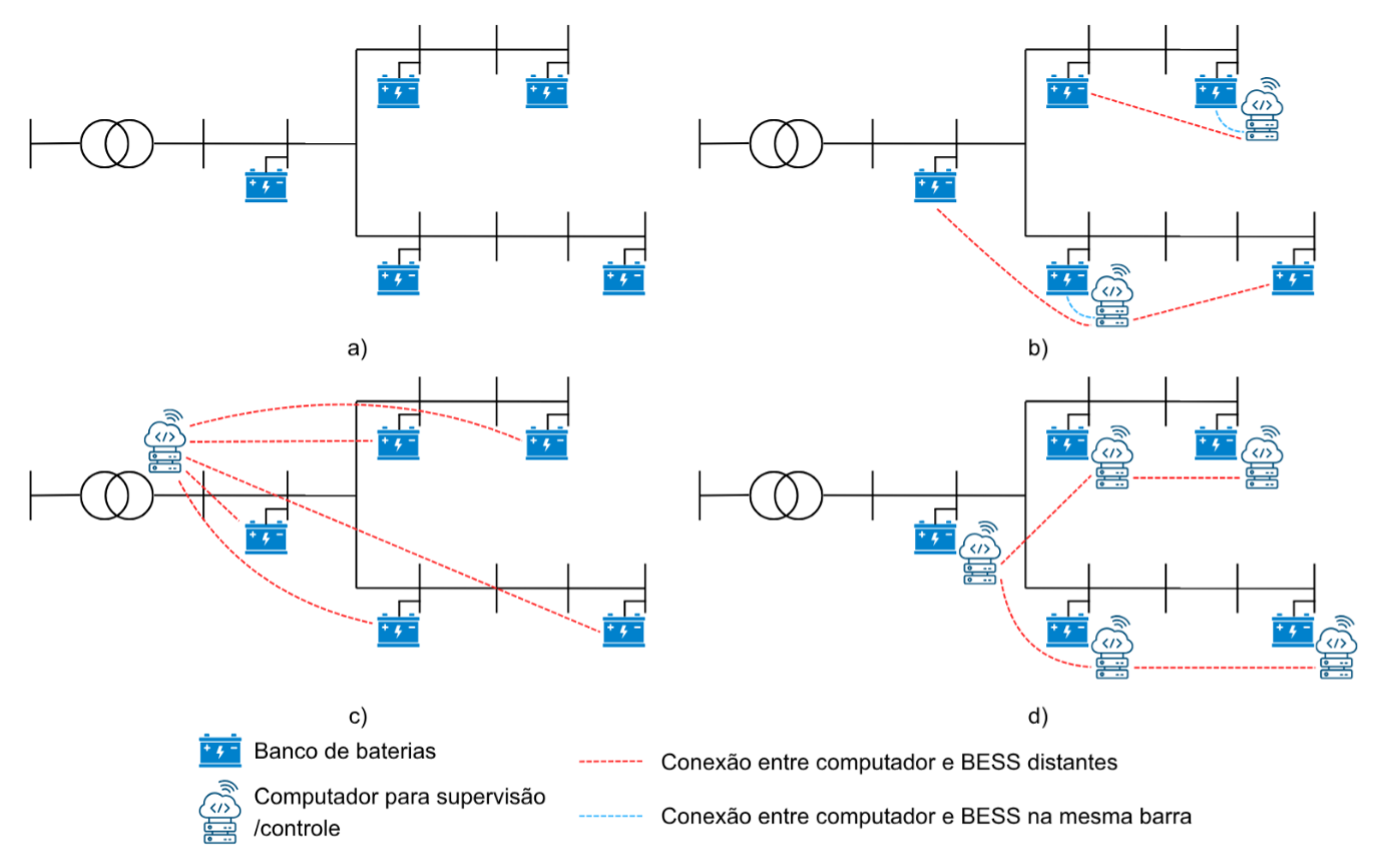
\includegraphics[width=0.85\textwidth]{arquiteturas_de_controle_distribuidos.png}
  \par\vspace{2pt}\fonte{adaptado de~\cite{stecca2020}}
\end{figure}

A aplicação do controle distribuído traz benefícios em relação às demais estratégias. Ele apresenta 
resiliência e robustez, uma vez que a falha de um nó não compromete todo o sistema~\cite{qiu2025}; 
escalabilidade, já que novos BESS podem ser adicionados com baixa latência de 
adaptação~\cite{freqreg2020,tdinterc2022}; e infraestrutura de comunicação entre vizinhos mais simples 
que a exigida pelas estratégias centralizadas. Em contrapartida, sua principal desvantagem é que a 
coordenação global ótima pode não ser atingida, pois nenhum agente dispõe da visão completa da rede.

\section{Estratégias de controle distribuído}
\label{sec:estrategias}

No contexto do controle distribuído, a literatura apresenta diversas formulações matemáticas, entre as 
quais se destacam o consenso~\cite{xing2022}, o método dos multiplicadores de direção alternada 
(\emph{Alternating Direction Method of Multipliers} --- ADMM)~\cite{far2023}, o controle preditivo 
distribuído (\emph{Distributed Model Predictive Control} --- DMPC)~\cite{ma2024}, o aprendizado por 
reforço multiagente (\emph{Multi-Agent Reinforcement Learning} --- MARL)~\cite{cao2021}, o controle 
estocástico de dupla camada~\cite{emarati2021}, a lógica \emph{fuzzy} distribuída~\cite{fuzzy2022} e a 
busca em árvore de Monte Carlo com aprendizado por reforço (\emph{Monte Carlo Tree Search} --- 
MCTS-RL)~\cite{alsaffar2020}. A seguir, sintetizam-se as contribuições de cada abordagem.

O controle distribuído por consenso~\cite{xing2022} mitiga sobretensões causadas por alta penetração FV 
em redes de baixa tensão considerando atrasos de comunicação. A estratégia combina uma ação local 
(\emph{droop}) com um algoritmo de consenso que estima médias globais da potência requerida e da 
capacidade máxima dos BESS, despachando a potência de forma proporcional ao estado de carga de cada 
unidade e, assim, distribuindo equitativamente o esforço de regulação. A otimização distribuída via 
ADMM~\cite{far2023} decompõe um problema centralizado em subproblemas locais resolvidos em paralelo por 
cada inversor inteligente, coordenando, em duas fases, o corte mínimo de potência ativa e o 
redirecionamento desse excedente para o carregamento dos BESS. O controle preditivo DMPC~\cite{ma2024} 
trata a incerteza da geração FV gerando cenários por Monte Carlo e resolvendo, de forma distribuída via 
ADMM, problemas de otimização que minimizam o custo das ações de controle em áreas de controle local. O 
aprendizado por reforço multiagente~\cite{cao2021} propõe regulação livre de modelo, com treinamento 
centralizado e execução descentralizada, particionando a rede em sub-regiões tratadas como agentes 
inteligentes.

O controle estocástico de dupla camada~\cite{emarati2021} coordena comutadores de tape sob carga, BESS e 
a compensação de reativos dos inversores FV em dois níveis temporais (agendamento diário e tempo real), 
modelando a incerteza solar por simulação de Monte Carlo. A lógica \emph{fuzzy} 
distribuída~\cite{fuzzy2022} embarca um controlador baseado em regras que recebe o desvio de tensão, o 
desvio de frequência e o estado de carga, considerando explicitamente a degradação das baterias e 
dividindo as unidades em grupos por estado de carga para evitar microciclos. Por fim, o controle 
heurístico MCTS-RL~\cite{alsaffar2020} combina um controlador preditivo descentralizado com um 
planejador centralizado por aprendizado por reforço que identifica ``regiões assistentes'' para 
receber a potência excedente, aumentando virtualmente a capacidade de armazenamento das regiões 
críticas.

A Tabela~\ref{tab:comparacao} sintetiza os métodos analisados, considerando o nível de tensão da rede estudada, a rede de teste e o papel desempenhado pelo BESS. Observa-se que a maioria dos trabalhos contempla redes de média tensão e que, em todas as estratégias, o BESS atua como atuador que injeta ou absorve a potência comandada pelo controle.

\begin{table}[!htb]
  \centering
  \caption{Síntese comparativa das estratégias de controle distribuído analisadas.}
  \label{tab:comparacao}
  \footnotesize
  \begin{tabular}{@{}llll@{}}
    \toprule
    \textbf{Ref.} & \textbf{Método} & \textbf{Rede de teste} & \textbf{Papel do BESS} \\
    \midrule
    \cite{xing2022}    & Consenso                  & Baixa tensão            & Absorve $P$ proporcional ao SoC \\
    \cite{far2023}     & PJ-ADMM                   & IEEE 13, 33 e 141 barras & Absorve excedente FV e injeta na ponta \\
    \cite{ma2024}      & DSMPC                     & IEEE 34 barras          & Absorve/injeta $P$ conforme controlador \\
    \cite{cao2021}     & MARL (MASDAC)             & IEEE 123 e 342 barras   & Absorve/injeta $P$ conforme controlador \\
    \cite{emarati2021} & Estocástico dupla camada  & Rede real 10\,kV, 37 barras & Agendamento diário e suporte de reativos \\
    \cite{fuzzy2022}   & FLC \emph{fuzzy}          & IEEE 33 barras          & Absorve/injeta $P$ e $Q$; grupos de SoC \\
    \cite{alsaffar2020} & MCTS-RL + MPC            & IEEE 33 barras e rede real & Compensa capacidade de regiões críticas \\
    \bottomrule
  \end{tabular}
  \par\vspace{2pt}\fonte{autoria própria}
\end{table}

\section{Algoritmos de consenso}
\label{sec:consenso}

A maior parte das estratégias de controle distribuído para BESS adota uma arquitetura hierárquica em 
duas camadas. A primeira camada (controle primário) é geralmente baseada em \emph{droop control}, 
responsável pela estabilidade local de tensão e frequência por meio de relações entre potência e tensão. 
Como essa abordagem introduz desvios em relação aos valores nominais, faz-se necessária uma camada 
secundária, na qual os algoritmos de consenso restauram a tensão média do sistema e coordenam o 
comportamento global dos BESS, ajustando as referências do controle primário.

Os algoritmos de consenso são amplamente utilizados em sistemas multiagentes para garantir que variáveis 
de interesse global --- como tensão, potência ou estado de carga (\emph{State of Charge} --- SoC) --- 
convirjam para valores comuns a partir de interações locais. A rede de comunicação entre os BESS é 
modelada como um grafo $G$, no qual cada unidade é um nó e as conexões são descritas por uma matriz de 
adjacência $A$. A partir dessa representação, define-se a matriz Laplaciana
\begin{equation}
  L = D - A,
  \label{eq:laplaciana}
\end{equation}
em que $D$ é a matriz de grau, que indica com quantos nós cada nó se relaciona. A matriz Laplaciana 
desempenha papel central na dinâmica do sistema e na convergência do algoritmo~\cite{tang2023}. A 
conectividade algébrica do grafo, associada ao segundo menor autovalor de $L$, denotado $\lambda_2$, 
determina diretamente a velocidade de convergência: uma conectividade muito baixa leva a convergência 
lenta, capaz de comprometer a resposta do sistema, enquanto uma conectividade excessivamente alta pode 
induzir instabilidades. Assim, o ajuste adequado dos parâmetros é essencial para garantir desempenho e 
robustez.

Além da regulação de tensão, os algoritmos de consenso são empregados para o balanceamento do SoC entre 
as unidades, evitando que algumas baterias sejam sobrecarregadas enquanto outras permanecem 
subutilizadas~\cite{li2026}. A literatura aponta, contudo, que os objetivos de regulação de tensão e de 
balanceamento de SoC são conflitantes: análises baseadas em critérios de estabilidade de Lyapunov 
indicam que esses objetivos podem levar o sistema a dois pontos de equilíbrio distintos, exigindo 
estratégias que conciliem ambas as demandas~\cite{tang2023}.

A estabilidade dos algoritmos de consenso costuma ser avaliada por meio de funções de Lyapunov, que 
quantificam o erro global e garantem a convergência. Quanto aos métodos de convergência, observa-se uma 
evolução temporal: trabalhos mais antigos empregam convergência em tempo finito (\emph{finite-time}), 
cujo tempo depende das condições iniciais~\cite{zhang2023,hu2019}; abordagens mais recentes priorizam o 
tempo fixo (\emph{fixed-time}), limitado por um valor superior independente do estado 
inicial~\cite{zeng2024,zhou2024}; e há ainda métodos de tempo prescrito (\emph{prescribed-time}), que 
permitem definir explicitamente o tempo de convergência~\cite{li2024}. Diversas extensões lidam com 
desafios práticos, como líderes virtuais~\cite{ren2022}, \emph{pinning control}~\cite{yang2018}, 
topologias variantes no tempo e resiliência a ataques ciberfísicos~\cite{zhou2024}, além de considerar 
heterogeneidade dos BESS, degradação e diferentes demandas de controle de 
frequência~\cite{wang2024,he2023}.

\section{Posicionamento do trabalho}
\label{sec:posicionamento}

A revisão evidencia que os algoritmos de consenso constituem a base das estratégias de controle 
distribuído para BESS, com a teoria dos grafos fornecendo o arcabouço matemático e a combinação entre 
controle primário (\emph{droop}) e secundário (consenso) consolidando-se como a arquitetura predominante. 
Nesse contexto, dois trabalhos orientam diretamente este projeto: o controle por consenso 
de~\cite{xing2022}, que comprova a eficácia da abordagem na distribuição equitativa do esforço de 
regulação entre os BESS, e o algoritmo de dupla camada de~\cite{paradacontzen2024}, tomado como 
referência para a solução implementada. O método de Monte Carlo, empregado em~\cite{emarati2021} para 
gerar cenários diários de geração, também é adotado neste trabalho, porém estendido à variação espacial 
e dimensional dos recursos.

Por fim, identificam-se as lacunas que o projeto pretende abordar ao longo de suas duas etapas: a 
ausência de análise do desempenho do controle distribuído em redes trifásicas desequilibradas e a 
desconsideração da degradação das baterias no laço de controle. Esses pontos, conforme delimitado na 
Seção~\ref{sec:objetivos}, integram o escopo da segunda etapa do projeto.

\chapter{Ambiente de simulação e redes de teste}
\label{cap:ambiente}

Este capítulo descreve a infraestrutura computacional desenvolvida para a execução das simulações e as 
redes de distribuição utilizadas. A rede IEEE~33 barras foi empregada para a validação inicial do 
ambiente, ao passo que a rede IEEE~34 barras, de maior porte e com elementos de regulação 
representativos, foi adotada como sistema de estudo nas etapas subsequentes.

\section{O software OpenDSS}
\label{sec:opendss}

O OpenDSS (\emph{Open Distribution System Simulator}), desenvolvido pelo 
\emph{Electric Power Research Institute} (EPRI)~\cite{dugan2020opendss}, é um simulador de propósito 
geral para análise de sistemas de distribuição, amplamente utilizado para o cálculo de fluxo de 
potência. A matriz de admitância do sistema, que relaciona correntes injetadas e tensões nodais, é 
montada a partir das matrizes de admitância primitivas de cada elemento e resolvida por um \emph{solver} 
de matrizes esparsas. O fluxo de potência, que determina as tensões em cada barra e os fluxos de 
potência ativa e reativa nas linhas, é calculado iterativamente pelo método de injeção de corrente 
(padrão), com o método de Newton disponível para circuitos de convergência mais difícil. Determinar o 
fluxo de potência é fundamental para avaliar o carregamento da rede, identificar violações de tensão e 
apoiar as decisões de controle.

\section{Integração Python--OpenDSS}
\label{sec:api}

A integração do OpenDSS com Python possibilita o desenvolvimento de ferramentas que exploram os 
resultados do fluxo de potência de forma programática e automatizada, viabilizando estudos de 
controladores de BESS em diferentes cenários. Para essa integração, avaliaram-se as interfaces de 
programação disponíveis. A abordagem oficial baseia-se na interface \emph{Component Object Model} 
(COM), de uso restrito ao Windows. Como alternativa multiplataforma, o projeto DSS-Extensions 
disponibiliza três bibliotecas Python --- DSS-Python, OpenDSSDirect.py e AltDSS-Python ---, todas 
construídas sobre o motor AltDSS, compatível com o OpenDSS oficial e com suporte a Windows, Linux e 
macOS.

Cabe registrar um ajuste em relação ao plano de trabalho, que previa a interface COM: optou-se pela 
biblioteca OpenDSSDirect.py. A escolha justifica-se por ser o pacote mais maduro entre as opções do 
DSS-Extensions, por oferecer uma interface por chamadas de função direta e bem documentada, adequada 
às iterações frequentes sobre elementos da rede exigidas pelas etapas de controle, e por disponibilizar 
funções utilitárias para conversão dos elementos da rede em estruturas de dados da biblioteca 
\emph{pandas}, facilitando a exportação e a análise dos resultados. Além disso, o suporte 
multiplataforma elimina a dependência do sistema operacional Windows.

\section{Validação na rede IEEE~33 barras}
\label{sec:ieee33}

A rede IEEE~33 barras é um sistema de distribuição radial de referência, proposto originalmente por 
Baran e Wu~\cite{baranwu1989}, com tensão nominal de 12,66~kV (média tensão), composto por 33 barras e 
32 ramais. A topologia é puramente radial, com uma barra de suprimento (barra~1, tomada como referência) 
e 32 barras de carga; a demanda total é de 3,715~MW de potência ativa, distribuída de forma não 
uniforme. As \emph{tie lines} originais, com chaves normalmente abertas, foram desconsideradas nesta 
simulação. A Figura~\ref{fig:ieee33} apresenta o diagrama unifilar da rede.

\begin{figure}[!htb]
  \centering
  \caption{Diagrama unifilar do sistema de testes IEEE~33 barras.}
  \label{fig:ieee33}
  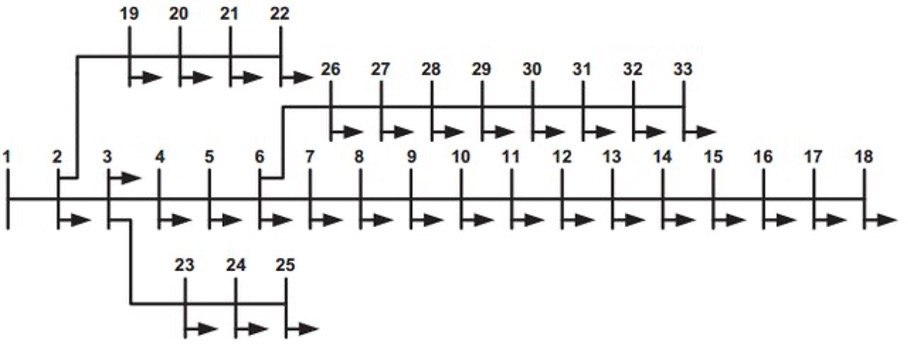
\includegraphics[width=0.92\textwidth]{diagrama_unifilar_33_barras.jpg}
  \par\vspace{2pt}\fonte{adaptado de~\cite{baranwu1989}}
\end{figure}

Para validar o ambiente, executou-se o fluxo de potência da rede em modo estático (\emph{snapshot}), 
com a rede operando a 100\% de sua carga nominal. Os resultados revelaram um perfil de tensão 
decrescente ao longo dos alimentadores, comportamento esperado em redes radiais com carga distribuída: 
a barra de suprimento apresenta tensão próxima da nominal, enquanto as barras mais distantes da 
subestação atingem valores inferiores ao limite de 0,95~p.u., com mínimo de 0,9059~p.u. na barra~18. 
As tabelas completas de tensões nodais e de fluxos de potência por linha encontram-se no 
Apêndice~\ref{ap:fluxo33}. A correta obtenção desses resultados validou o ambiente de cossimulação e 
estabeleceu a infraestrutura necessária para as etapas de controle. Cabe registrar que a rede IEEE~33 
barras foi empregada apenas nessa validação inicial; melhorias propostas na literatura, como a inclusão 
de geração distribuída, compensadores de reativos e curvas de carga~\cite{ghorbanian2019}, motivaram a 
adoção da rede IEEE~34 barras como sistema de estudo nas etapas seguintes.

\section{Rede de estudo: IEEE~34 barras}
\label{sec:ieee34}

A partir da validação do ambiente, adotou-se a rede \emph{IEEE 34 Bus Test Feeder} como sistema de 
estudo, por ser um alimentador de média tensão amplamente utilizado na avaliação de algoritmos de 
controle, fluxo de potência e integração de recursos distribuídos, e por incorporar dispositivos de 
regulação representativos de redes reais. A Figura~\ref{fig:ieee34} apresenta o diagrama da rede.

\begin{figure}[!htb]
  \centering
  \caption{Diagrama da rede IEEE~34 barras, com indicação das categorias de carga.}
  \label{fig:ieee34}
  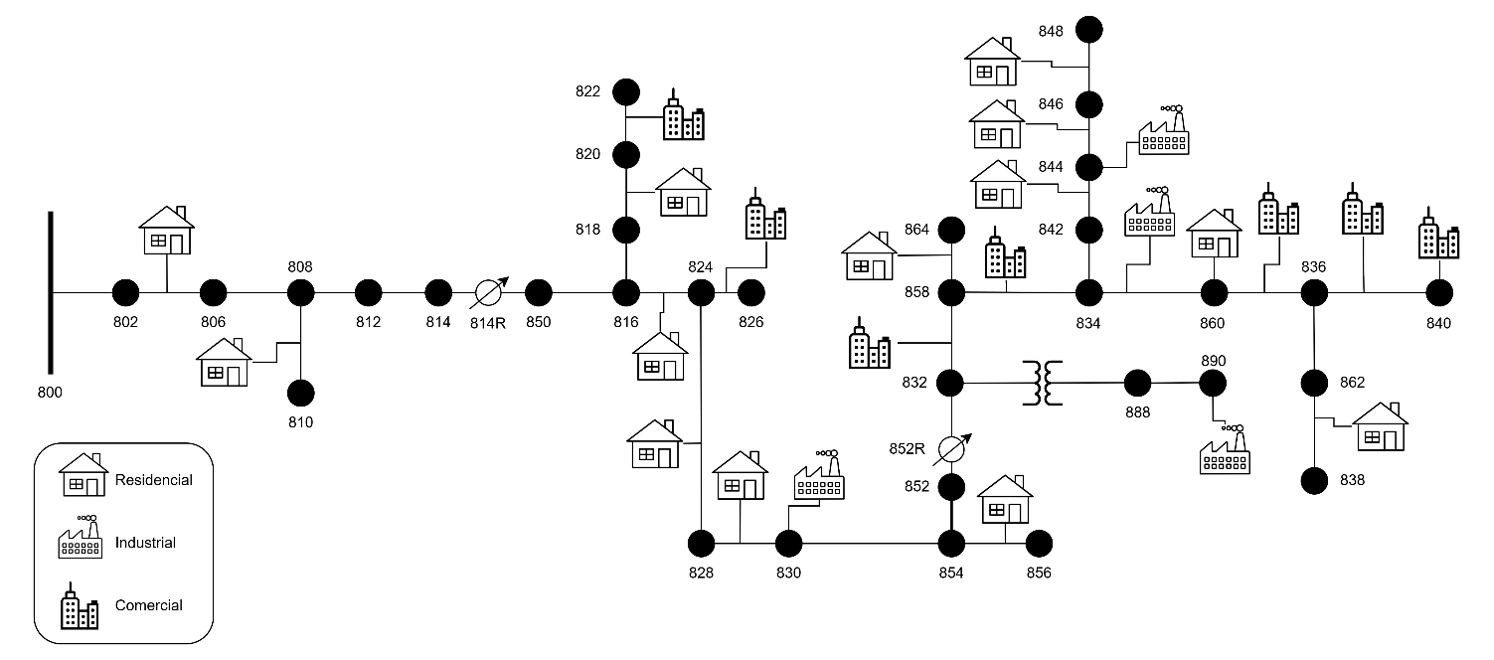
\includegraphics[width=\textwidth]{diagrama_unifilar_34_barras.png}
  \par\vspace{2pt}\fonte{autoria própria}
\end{figure}

A alimentação é feita a partir de uma subestação conectada à barra principal por um transformador 
abaixador trifásico de 25~MVA e relação 69/24,9~kV, com impedância de curto-circuito reduzida, de modo 
a tornar a fonte suficientemente rígida para os estudos de penetração de GD. A rede opera 
predominantemente em 24,9~kV, com exceção de um ramal (barras 888 e 890) alimentado por um segundo 
transformador de 500~kVA e relação 24,9/4,16~kV. A topologia é radial, com trechos trifásicos e 
monofásicos; as 32 linhas são definidas a partir dos códigos de impedância de fase padronizados pelo 
IEEE.

Para o controle de tensão ao longo do alimentador, a rede possui dois bancos reguladores com controle 
independente por fase: o primeiro, entre as barras 814 e 814R, opera com tensão de referência de 122~V 
e banda de 2~V; o segundo, entre as barras 852 e 852R, é ajustado para 124~V. Ambos foram modelados 
como transformadores monofásicos de enrolamento duplo com controle automático de tap via o elemento 
\emph{RegControl} do OpenDSS. Há ainda dois bancos de capacitores \emph{shunt} nas barras 844 e 848, 
que contribuem para o suporte de tensão nas regiões mais afastadas da subestação. As cargas dividem-se 
em concentradas (\emph{spot loads}), nas barras 860, 840, 844, 848, 830 e 890, e distribuídas, 
alocadas nas barras de origem e destino de cada segmento; a carga de pico total é de 1,769~MW e a 
demanda reativa total, de 1,044~MVAr.

\subsection{Perfis de carga}
\label{sec:perfis_carga}

À rede original foram acrescentados três perfis de carga horária --- residencial, comercial e industrial 
--- com resolução de uma hora e horizonte de 24~horas, representando o comportamento típico de cada 
categoria de consumidor. Cada carga foi então associada a um desses perfis, de modo que a demanda a 
cada hora é obtida multiplicando o fator de carga horário pela demanda máxima da carga. 
A Figura~\ref{fig:perfis_carga} ilustra os três perfis. O perfil residencial caracteriza-se por 
consumo reduzido na madrugada e pico por volta das 20~h; o comercial apresenta consumo elevado entre 
9~h e 12~h, cedendo à noite; e o industrial distingue-se dos demais por apresentar fatores
multiplicativos superiores à unidade entre 9~h e 12~h, indicando que a potência nominal declarada
corresponde a uma condição de carga parcial, superada durante o turno de operação plena. Foram 
classificadas como residenciais as cargas das barras 848 e 860; como comerciais, as das barras 820, 
822, 824, 826, 832, 836, 840 e 858; e como industriais, as das barras 830, 834, 844 e 890. As demais 
cargas distribuídas, de menor expressão, foram tratadas como residenciais.

\begin{figure}[!htb]
  \centering
  \caption{Curvas de carga típicas (residencial, comercial e industrial).}
  \label{fig:perfis_carga}
  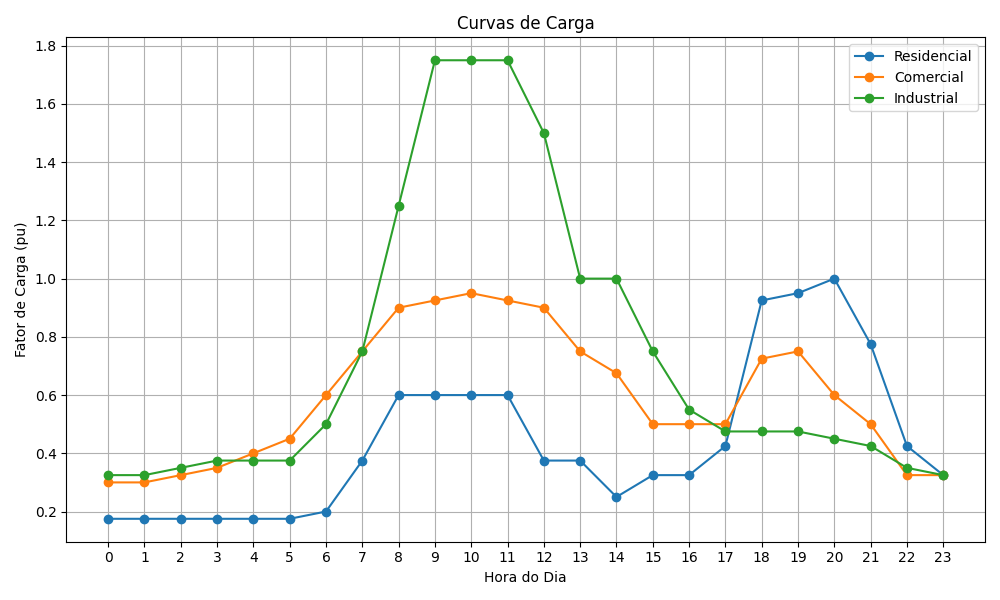
\includegraphics[width=0.75\textwidth]{curvas_carga.png}
  \par\vspace{2pt}\fonte{autoria própria}
\end{figure}

\chapter{Geração de cenários por Monte Carlo}
\label{cap:cenarios}

O objetivo desta etapa é construir um conjunto representativo de configurações operacionais da rede IEEE~34 barras sob diferentes condições de inserção de geração fotovoltaica e de BESS, permitindo a avaliação probabilística do impacto desses recursos sobre os perfis de tensão. As configurações incluem o nível de penetração FV, a distribuição espacial e o dimensionamento das unidades FV e BESS, o tipo de dia e o respectivo perfil de irradiância, e o perfil de carga da rede.

\section{O método de Monte Carlo}
\label{sec:montecarlo}

A simulação de Monte Carlo é uma técnica numérica que, em contraste com abordagens determinísticas, incorpora explicitamente as incertezas do sistema por meio de distribuições de probabilidade. Cada variável é associada à sua distribuição; para cada cenário, os valores são sorteados aleatoriamente e empregados na execução do modelo. Repetindo-se o procedimento um número elevado de vezes, obtém-se não um único resultado determinístico, mas uma distribuição de comportamentos possíveis, a partir da qual se calculam estatísticas descritivas --- média, desvio padrão, percentis e probabilidade de violação de limites.

Para a avaliação do impacto de cada cenário sobre os perfis de tensão ao longo de um dia, emprega-se a simulação de fluxo de potência quasi-estática~\cite{cunha2021}, executada em patamares horários ao longo das 24~horas, capturando a variação temporal da geração FV e da demanda. O procedimento se organiza em três etapas: (i)~geração dos cenários pelo método de Monte Carlo, sorteando combinações de localização e potência dos sistemas FV, capacidade dos BESS e perfis de irradiância e carga; (ii)~simulação do fluxo de potência de cada cenário no OpenDSS, extraindo os perfis de tensão de todas as barras; e (iii)~análise estatística dos resultados, consolidados por nível de penetração.

As variáveis estocásticas dividem-se em quatro grupos: a alocação e o dimensionamento das unidades FV; a alocação e o dimensionamento das unidades BESS; o perfil de irradiância solar; e os fatores de incerteza aplicados aos perfis de carga. O nível de penetração fotovoltaica, $\eta$, é definido como a razão entre a potência nominal total instalada dos sistemas FV e a demanda de pico total da rede. Foram considerados onze níveis, de 0\% a 100\% em incrementos de 10\%, com 500~cenários independentes por nível, totalizando 5500~cenários simulados.

\section{Alocação e dimensionamento dos sistemas FV}
\label{sec:alocacao_fv}

Os sistemas FV foram restritos às barras que alimentam cargas trifásicas do alimentador (barras 860, 840, 844, 848 e 890), evitando o desequilíbrio que uma injeção monofásica de grande magnitude introduziria na rede. A potência nominal total dos sistemas FV de cada cenário é determinada diretamente pelo nível de penetração $\eta$ e pela demanda de pico $P_\text{pico} = 1{,}769$~MW, conforme a Equação~\eqref{eq:pfv_total}:
\begin{equation}
  P_\text{FV}^\text{total} = P_\text{pico}\,\eta.
  \label{eq:pfv_total}
\end{equation}

A distribuição de $P_\text{FV}^\text{total}$ entre as barras segue uma alocação proporcional com perturbação gaussiana controlada, adotada para evitar que a variabilidade espacial domine a variância dos resultados de tensão. Cada uma das $N=5$ barras trifásicas elegíveis recebe uma fração $w_j$ da potência total, obtida pela normalização de um fator multiplicativo $g_j$ sorteado de forma independente, segundo as Equações~\eqref{eq:fv_aloc}:
\begin{subequations}
  \label{eq:fv_aloc}
  \begin{align}
    g_j &\sim \mathcal{N}(1{,}0,\ \sigma_\text{aloc}^2), \qquad g_j \in [0{,}5;\ 1{,}5], \label{eq:fv_g}\\
    w_j &= \frac{g_j}{\sum_{k=1}^{N} g_k}, \label{eq:fv_w}\\
    P_{\text{FV},j} &= P_\text{FV}^\text{total}\, w_j. \label{eq:fv_pj}
  \end{align}
\end{subequations}
O fator $g_j$ é truncado ao intervalo $[0{,}5;\ 1{,}5]$, de modo que nenhuma barra receba menos de 0,5 nem mais de 1,5 vez a fração média; a variância $\sigma_\text{aloc}^2$ controla a dispersão espacial da potência FV. A normalização em~\eqref{eq:fv_w} garante que os pesos somem a unidade, redistribuindo a potência total sem alterar o montante instalado.

\section{Alocação e operação dos BESS}
\label{sec:alocacao_bess}

Assim como os sistemas FV, as unidades BESS foram restritas às barras trifásicas. A potência nominal total do conjunto de BESS é fixada como fração de 35\% da potência FV total instalada, conforme a Equação~\eqref{eq:bess_total}:
\begin{equation}
  P_\text{BESS}^\text{total} = 0{,}35\, P_\text{FV}^\text{total}.
  \label{eq:bess_total}
\end{equation}
Essa regra garante que a capacidade de armazenamento cresça proporcionalmente à geração FV instalada, coerente com o objetivo dos BESS de absorver o excedente diurno e fornecer energia no pico noturno. A potência $P_\text{BESS}^\text{total}$ é distribuída entre as cinco barras trifásicas pelo mesmo mecanismo proporcional com perturbação gaussiana adotado para a alocação FV, com $\sigma_\text{BESS} = 0{,}10$.

Nesta etapa, o modelo de fluxo de potência não rastreia o estado de carga das baterias ao longo do tempo: o BESS é tratado como uma fonte ou carga de potência controlada, com perfil de operação determinístico e idêntico para todos os cenários e níveis de penetração. Esse perfil, $b(h)$, é definido pela Equação~\eqref{eq:bess_perfil}:
\begin{equation}
  b(h) =
  \begin{cases}
    -1{,}0, & h \in [10,\ 14] \quad \text{(carregamento)},\\
    +1{,}0, & h \in [18,\ 21] \quad \text{(descarregamento)},\\
    0{,}0,  & \text{caso contrário},
  \end{cases}
  \label{eq:bess_perfil}
\end{equation}
de modo que a potência efetiva absorvida ou injetada pela unidade da barra $j$ na hora $h$ é $P_{\text{BESS},j}(h) = P_{\text{BESS},j}\, b(h)$. A Figura~\ref{fig:perfil_bess} ilustra a curva de carregamento e descarregamento. Trata-se de uma simplificação desta etapa; um despacho otimizado em tempo real é objeto das etapas subsequentes do projeto.

\begin{figure}[!htb]
  \centering
  \caption{Curva de carregamento e descarregamento das unidades BESS.}
  \label{fig:perfil_bess}
  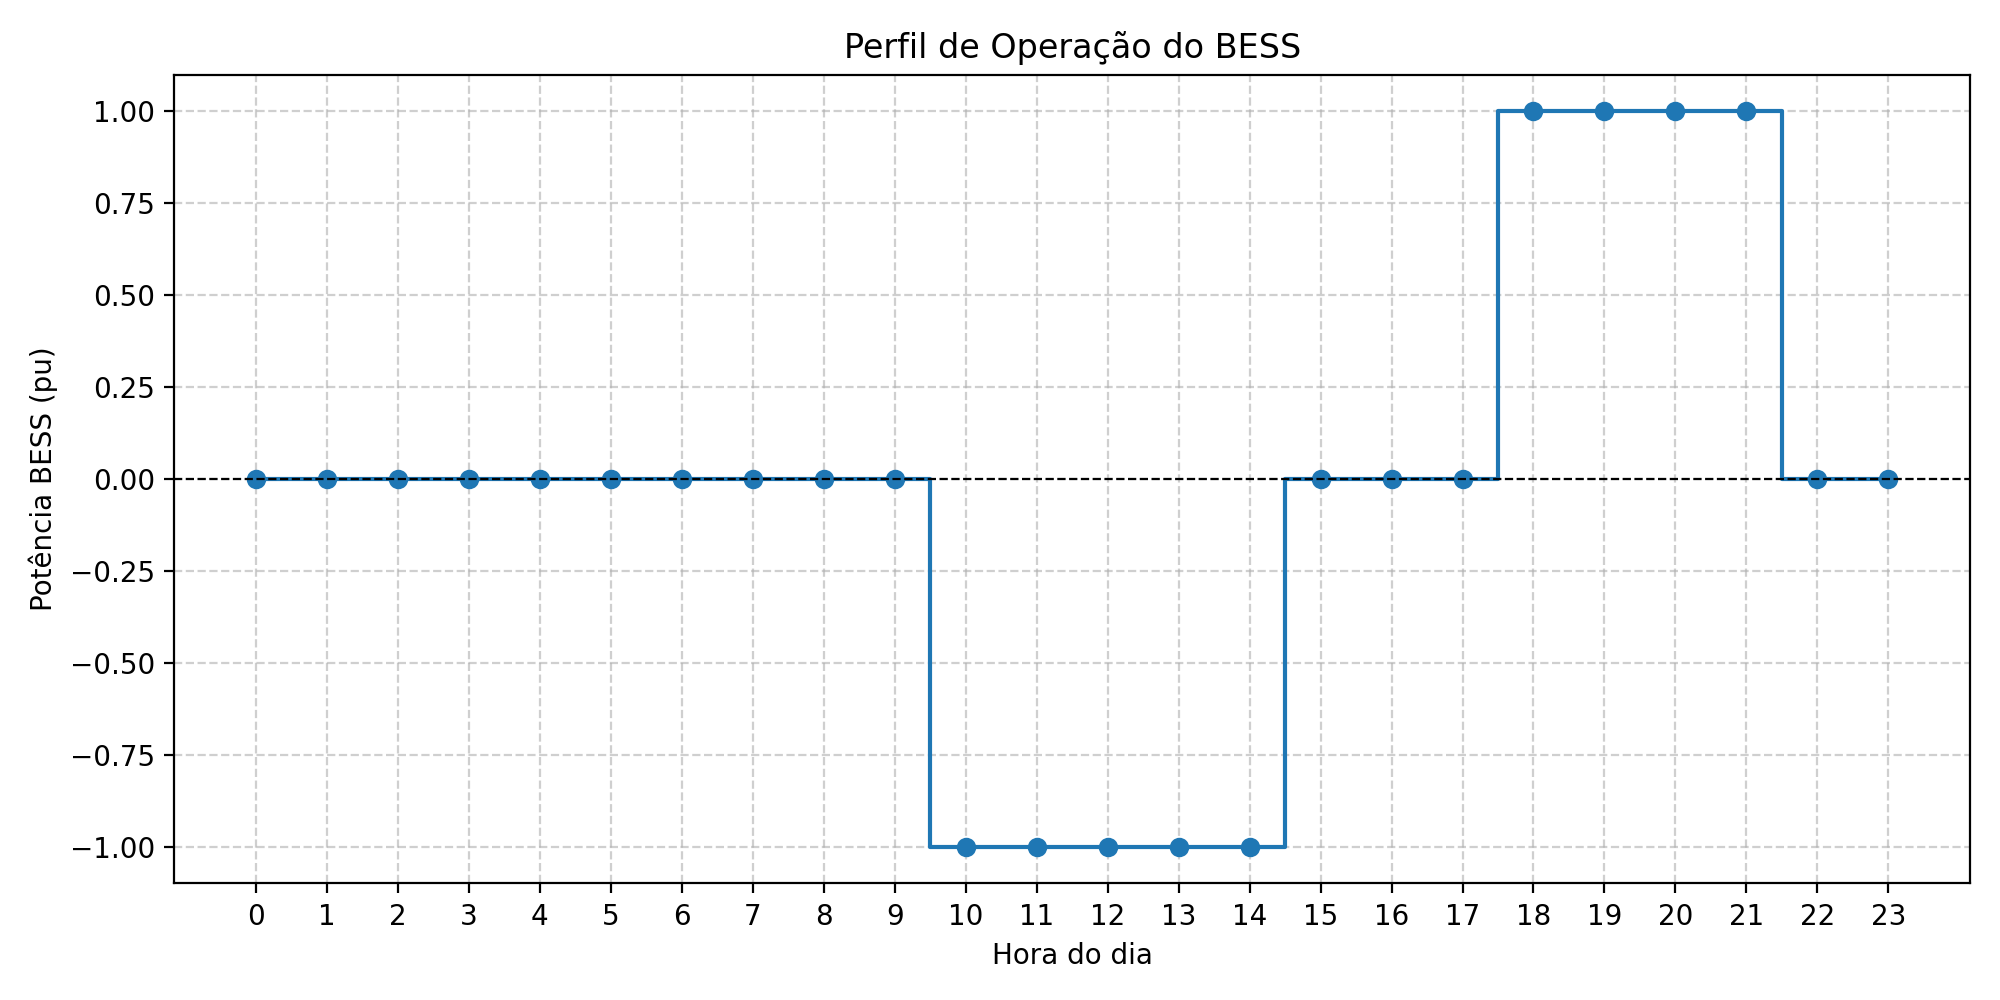
\includegraphics[width=0.72\textwidth]{perfil_bess.png}
  \par\vspace{2pt}\fonte{autoria própria}
\end{figure}

\section{Dia típico e perfil de irradiância}
\label{sec:irradiancia}

Para a geração dos perfis de irradiância, adotou-se um padrão misto que combina a categorização de dias típicos com o acréscimo de ruído gaussiano. A base de dados é proveniente do Sistema de Organização Nacional de Dados Ambientais (SONDA), operado pelo INPE~\cite{inpe_sonda}; utilizaram-se medições da estação de Cachoeira Paulista (SP) entre janeiro de 2023 e dezembro de 2025, tratadas para a remoção de valores espúrios e de dias incompletos.

A modelagem de dias típicos baseia-se no índice de claridade, definido na Equação~\eqref{eq:kt} como a razão entre a irradiância global horizontal integrada diariamente na superfície ($H$) e a irradiância extraterrestre teórica para o mesmo dia e local ($H_0$)~\cite{lai2017}:
\begin{equation}
  k_t = \frac{H}{H_0}.
  \label{eq:kt}
\end{equation}
Com base em $k_t$, definiram-se três dias típicos --- Céu Aberto, Parcialmente Nublado e Nublado ---, conforme a Tabela~\ref{tab:dias_tipicos}. A frequência de ocorrência de cada classe no período analisado (Figura~\ref{fig:kt}) foi utilizada como probabilidade no sorteio do tipo de dia em cada cenário.

\begin{table}[!htb]
  \centering
  \caption{Classificação dos dias típicos com base no índice de claridade $k_t$.}
  \label{tab:dias_tipicos}
  \begin{tabular}{@{}ll@{}}
    \toprule
    \textbf{Dia típico} & \textbf{Índice de claridade} \\
    \midrule
    Céu Aberto            & $k_t > 0{,}6$ \\
    Parcialmente Nublado  & $0{,}3 < k_t < 0{,}6$ \\
    Nublado               & $k_t < 0{,}3$ \\
    \bottomrule
  \end{tabular}
  \par\vspace{2pt}\fonte{autoria própria}
\end{table}

\begin{figure}[!htb]
  \centering
  \caption{Distribuição do índice de claridade no período analisado.}
  \label{fig:kt}
  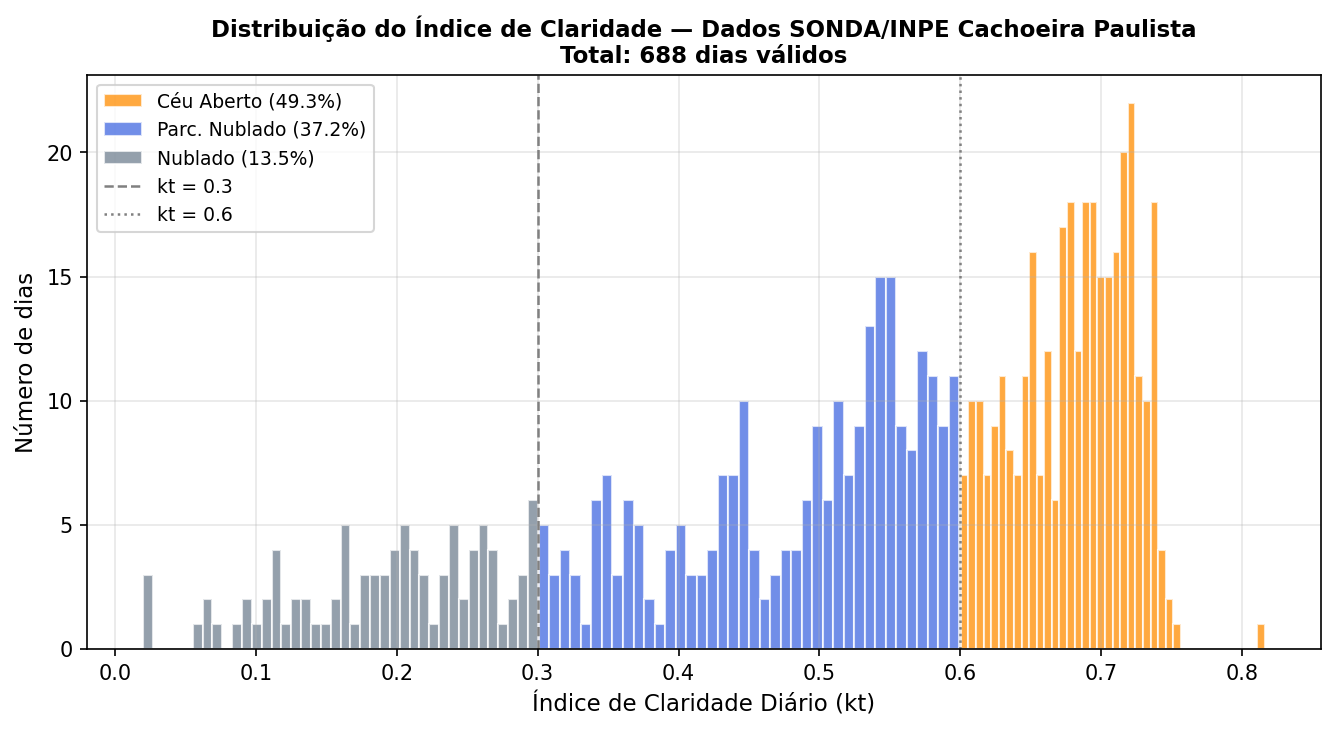
\includegraphics[width=0.7\textwidth]{sonda_classificacao_kt.png}
  \par\vspace{2pt}\fonte{autoria própria}
\end{figure}

Para cada dia típico, obteve-se a curva de irradiância diária por hora, normalizada pelo respectivo valor máximo para eliminar o efeito da variação sazonal (Figura~\ref{fig:perfis_irradiancia}). O perfil de céu aberto apresenta curva simétrica, com máximo próximo de 0,98~p.u. ao meio-dia solar; o parcialmente nublado é semelhante em forma, com amplitude ligeiramente menor; e o nublado exibe valores significativamente menores e distribuição mais achatada.

\begin{figure}[!htb]
  \centering
  \caption{Perfis horários típicos de irradiância normalizada.}
  \label{fig:perfis_irradiancia}
  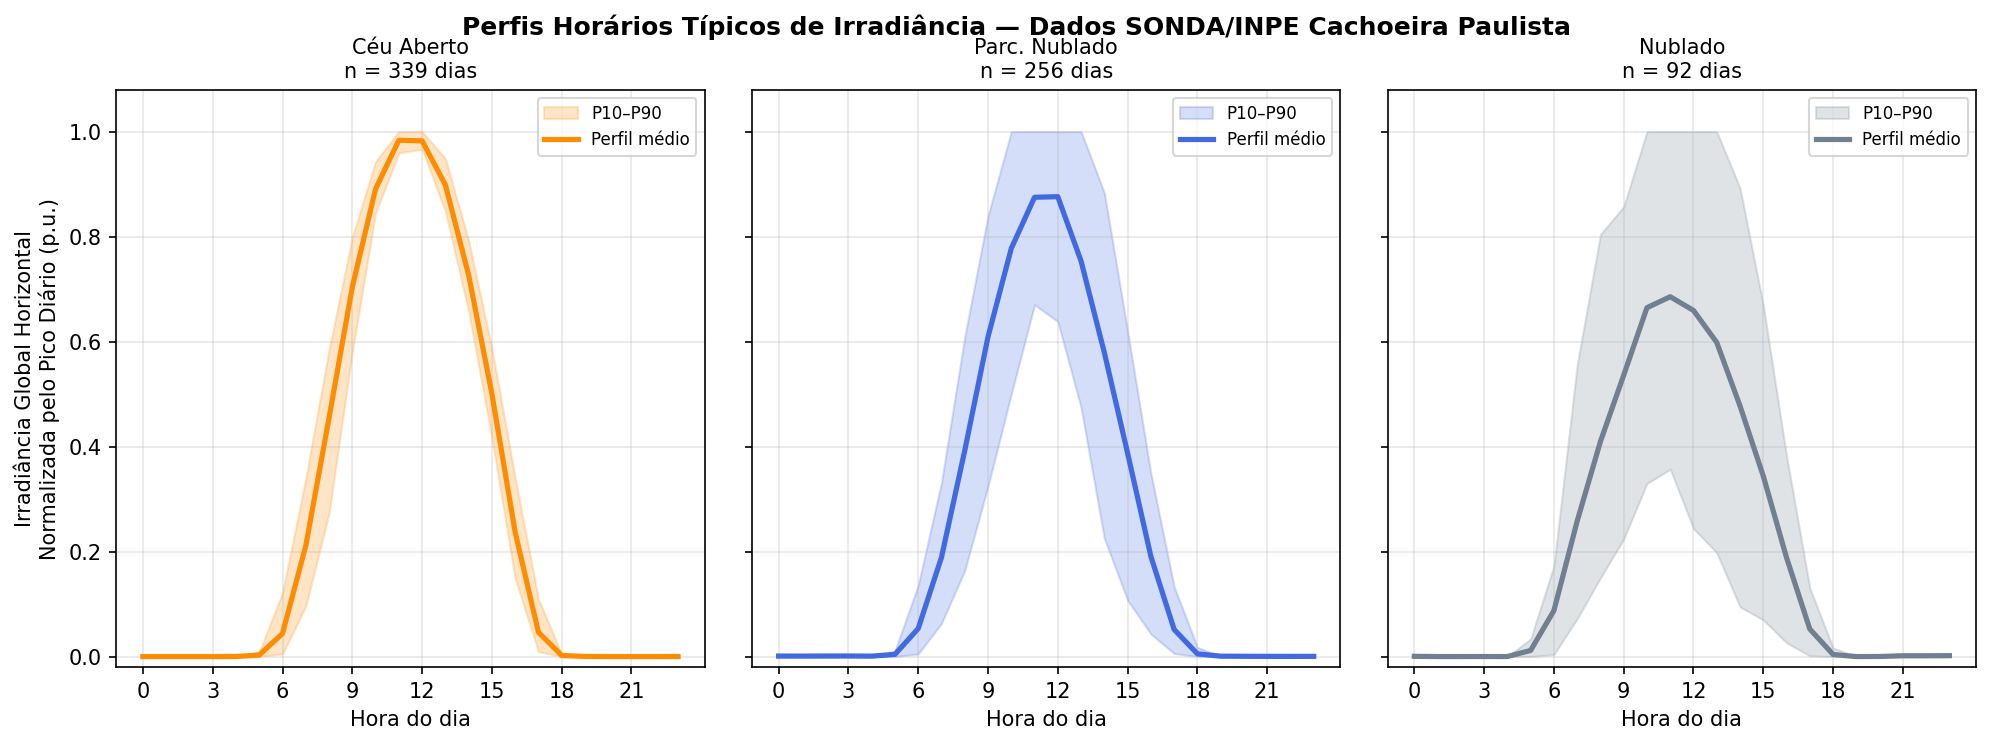
\includegraphics[width=0.7\textwidth]{sonda_perfis_irradiancia.png}
  \par\vspace{2pt}\fonte{autoria própria}
\end{figure}

Uma vez sorteado o tipo de dia, o perfil de irradiância do cenário $s$ é gerado introduzindo um ruído multiplicativo gaussiano hora a hora sobre o perfil médio correspondente, $\bar{I}(h)$, conforme a Equação~\eqref{eq:irradiancia}:
\begin{equation}
  I_s(h) = \operatorname{clip}\!\big[\,\bar{I}(h)\,(1 + \varepsilon(h)),\ 0,\ 1\,\big], \qquad \varepsilon(h) \sim \mathcal{N}(0,\ \sigma_i^2),
  \label{eq:irradiancia}
\end{equation}
em que $\varepsilon(h)$ é um ruído independente para cada hora, com desvio padrão relativo $\sigma_i$ inversamente proporcional ao índice de claridade --- quanto menor a claridade, maior a variabilidade ---, e a operação $\operatorname{clip}$ mantém o fator no intervalo fisicamente admissível $[0,\ 1]$. O mesmo perfil $I_s(h)$ é aplicado a todas as unidades FV de um dado cenário, hipótese de correlação espacial perfeita razoável para a extensão limitada da rede. A potência injetada por uma unidade de potência nominal $P_\text{FV}$ na hora $h$ é, portanto, $P_{\text{FV},s}(h) = P_\text{FV}\, I_s(h)$.

\section{Perfil de carga estocástico}
\label{sec:carga_estocastica}

Sobre os perfis de carga determinísticos descritos na Seção~\ref{sec:perfis_carga}, sobrepõe-se, em cada cenário, uma variabilidade estocástica. Para cada uma das barras de carga sorteia-se um fator multiplicativo $f_b$ a partir de uma distribuição normal de desvio padrão relativo $\sigma_d = 0{,}1$, truncado ao intervalo $[0{,}80;\ 1{,}20]$, conforme a Equação~\eqref{eq:carga}:
\begin{equation}
  f_b \sim \mathcal{N}(1{,}0,\ \sigma_d^2), \qquad f_b \in [0{,}80;\ 1{,}20].
  \label{eq:carga}
\end{equation}
Esse fator, mantido constante ao longo do dia para cada barra, representa a heterogeneidade entre consumidores. A potência efetiva na barra $b$ na hora $h$ resulta de $P_b(h) = P_b^\text{nom}\, f_b\, c(h)$, em que $P_b^\text{nom}$ é a potência nominal da barra e $c(h)$ o respectivo perfil de carga horário. Os fatores são sorteados de forma independente entre barras, o que implica ausência de correlação espacial na incerteza de demanda --- simplificação conservadora justificada pelo objetivo de gerar cenários-base para a avaliação do impacto da penetração FV.

\chapter{Estratégia de controle distribuído em duas camadas}
\label{cap:controle}

Este capítulo formaliza a estratégia de controle adotada, composta por duas camadas que atuam sobre variáveis distintas do inversor. A camada primária realiza a regulação local de tensão por meio da potência reativa, enquanto a camada secundária coordena os BESS por meio da potência ativa, empregando um algoritmo de consenso.

%\section{Arquitetura e separação de variáveis}
%\label{sec:arquitetura_controle}

O controle primário atua localmente em cada recurso energético distribuído (RED) ajustando a potência reativa $Q$ em função da tensão na barra, conforme a curva volt-var. O controle secundário atua exclusivamente sobre a potência ativa $P$ dos BESS, adicionando um sinal de correção $\Delta P$ calculado pelo algoritmo de consenso. Como as camadas operam em variáveis ortogonais do inversor --- $Q$ e $P$, respectivamente ---, não há conflito direto de atuação, o que permite a operação simultânea de ambas. Para preservar o fator de potência estabelecido pelo primário, a correção $\Delta P$ é acompanhada de uma correção proporcional de potência reativa $\Delta Q$, de modo a manter o ângulo de potência aparente vigente em cada BESS.

\section{Controle primário por curva volt-var}
\label{sec:primario}

A camada primária baseia-se na curva volt-var definida pela norma ABNT~NBR~16149:2013~ \cite{nbr16149}, que estabelece a potência reativa a ser injetada ou absorvida pelo inversor em função da tensão medida na barra de monitoramento. Adicionalmente, a função foi aplicada aos inversores de todos os REDs (FV e BESS), e não apenas aos BESS, ampliando a capacidade total de suporte de reativos sem custo adicional de comunicação.

A curva adotada, apresentada na Figura~\ref{fig:voltvar}, é definida por quatro pontos e três regiões. O limite de reativos foi fixado em $Q_\text{max} = 0{,}4358\,P_\text{inst}$, em conformidade com o limite de $\pm 43{,}58\%$ de $Q/P_N$ estabelecido pela norma; numericamente, $0{,}4358 = \operatorname{sen}(\arccos 0{,}90)$, valor correspondente à máxima injeção ou absorção de reativos sob fator de potência de 0,90. As três regiões são:
\begin{itemize}
  \item \textbf{zona morta} ($0{,}97 \le V \le 1{,}03$~p.u.): nenhuma potência reativa é injetada ou absorvida;
  \item \textbf{região capacitiva} ($V < 0{,}97$~p.u.): a injeção de reativos cresce linearmente de zero até $+Q_\text{max}$, atingido em 0,90~p.u.; abaixo disso, mantém-se $Q = +Q_\text{max}$;
  \item \textbf{região indutiva} ($V > 1{,}03$~p.u.): a absorção de reativos cresce linearmente de zero até $-Q_\text{max}$, atingida em 1,10~p.u.; acima disso, mantém-se $Q = -Q_\text{max}$.
\end{itemize}

\begin{figure}[!htb]
  \centering
  \caption{Curva volt-var adotada para o controle primário, conforme a ABNT~NBR~16149:2013.}
  \label{fig:voltvar}
  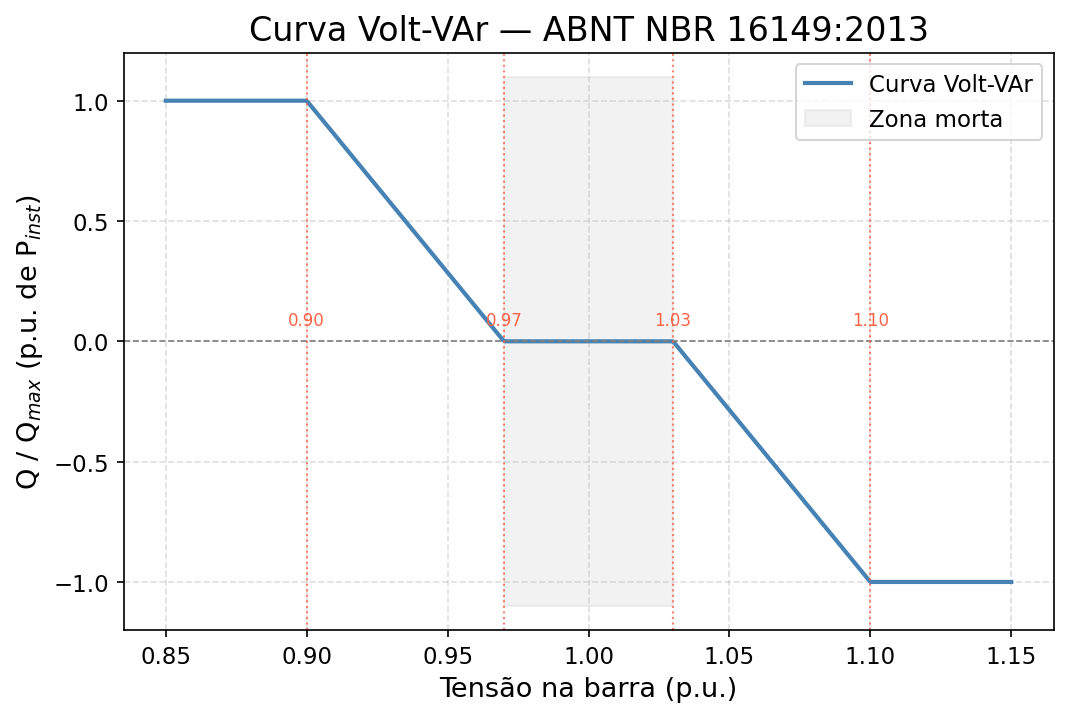
\includegraphics[width=0.72\textwidth]{volt_var_curve.png}
  \par\vspace{2pt}\fonte{adaptado de~\cite{nbr16149}}
\end{figure}

A implementação consiste em um laço de controle externo em Python, com dois 
\emph{solves} em modo \emph{snapshot} por hora no OpenDSS. No primeiro \emph{solve}, 
com os reguladores livres, registram-se as posições de tap após a convergência; em 
seguida, para cada RED, lê-se a tensão das fases da barra e calcula-se a referência 
de reativos pela curva volt-var, priorizando a violação mais crítica (maior desvio 
em relação à zona morta). O valor de $Q_\text{max}$ é proporcional à potência ativa 
instantânea do RED, de modo que inversores com geração parcial contribuem 
proporcionalmente, mantendo o fator de potência mínimo de 0,90. Caso ao menos um 
RED saia da zona morta, a posição dos taps dos reguladores de tensão é mantida 
inalterada (premissa de que a resposta 
de reativos do inversor é mais rápida que a comutação mecânica dos reguladores) e 
executa-se um segundo \emph{solve} no mesmo patamar horário, com a referência de 
reativos aplicada, ou seja, com um novo fator de potência.

\section{Controle secundário por consenso}
\label{sec:secundario}

\subsection{Topologia de comunicação}
\label{sec:topologia}

A rede de comunicação entre os BESS é modelada como um grafo esparso não dirigido $G = (V, E)$, em que cada nó representa um BESS e cada aresta uma vizinhança elétrica no alimentador: dois BESS são vizinhos quando não há outro BESS intermediário no caminho elétrico entre eles. Para as cinco barras trifásicas elegíveis, o grafo resulta na cadeia linear $860\text{--}840\text{--}844\text{--}848\text{--}890$. A partir da matriz de adjacência $A$, com pesos unitários, define-se a matriz Laplaciana $L = D - A$, cuja conectividade algébrica $\lambda_2$ governa a velocidade de convergência (Seção~\ref{sec:consenso}). Como o grafo é uma cadeia linear, garante-se $\lambda_2 > 0$ sempre que houver ao menos dois BESS no cenário; cenários com um único BESS, ou nenhum, não possuem grafo válido e o controle secundário é automaticamente desativado.

\subsection{Variável de consenso aumentada e lei de controle}
\label{sec:lei_controle}

A variável de consenso de cada BESS $i$ é a sua potência ativa normalizada pela potência nominal, acrescida de um termo proporcional ao desvio de tensão na barra de instalação, conforme a Equação~\eqref{eq:x_consenso}:
\begin{equation}
  x_i = \frac{P_i}{P_{\text{nom},i}} + \gamma\,(V_\text{ref} - V_i),
  \label{eq:x_consenso}
\end{equation}
em que $P_i$ é a potência ativa vigente, $V_i$ a tensão média 
entre as fases da barra, $V_\text{ref} = 1{,}0$~p.u. a tensão 
de referência e $\gamma = 2{,}0$ o peso do termo de tensão. 
Conceitualmente, $x_i$ é a grandeza que o algoritmo de consenso 
busca igualar entre os BESS vizinhos. Ao equalizar $x_i$, os 
BESS compartilham o esforço de regulação de forma proporcional 
à sua capacidade (parcela $P_i/P_{\text{nom},i}$, que mede o 
quanto da potência nominal cada unidade está utilizando) e, ao 
mesmo tempo, direcionam mais correção às barras com maior desvio 
de tensão (parcela $\gamma\,(V_\text{ref} - V_i)$). Esse 
segundo termo introduz heterogeneidade entre os BESS conforme 
as condições locais de tensão: sem ele, o consenso convergiria 
trivialmente sem produzir correção útil.

A lei de controle distribuído calcula, para cada BESS $i$, um sinal de correção de potência ativa $\Delta P_i$ composto por uma parcela de consenso e uma parcela de \emph{droop}, conforme a Equação~\eqref{eq:dp}:
\begin{equation}
  \Delta P_i = -\alpha\, P_{\text{nom},i}\, [L x]_i + \Delta P_{\text{droop},i},
  \label{eq:dp}
\end{equation}
em que $\alpha = 0{,}15$ é o ganho do consenso e $[L x]_i$ é a $i$-ésima componente do produto da matriz Laplaciana pelo vetor de variáveis de consenso. Adota-se a convenção de carga, na qual $\Delta P < 0$ corresponde a maior injeção de potência ativa na rede. A parcela puramente Laplaciana possui, por construção, soma nula entre os nós, de modo que o consenso isolado apenas redistribui a potência ativa entre os BESS, sem alterar o balanço agregado de injeção.

A parcela de \emph{droop}, calculada localmente a partir da tensão da barra, segue a mesma lógica de zona morta e saturação do controle primário, conforme a Equação~\eqref{eq:droop}:
\begin{equation}
  \Delta P_{\text{droop},i} = k_\text{droop}\, P_{\text{nom},i}\,(V_i - V_\text{db}), \qquad \text{com saturação em } \pm P_{\text{nom},i},
  \label{eq:droop}
\end{equation}
em que $V_\text{db}$ é o limiar de zona morta mais próximo (0,97~p.u. em subtensão ou 1,03~p.u. em sobretensão) e $k_\text{droop}$ é calculado de modo que a correção atinja a saturação $\pm P_{\text{nom},i}$ exatamente nos limites de saturação de tensão do controle primário (0,90 e 1,10~p.u.):
\begin{equation}
  k_\text{droop} = \frac{1}{1{,}10 - 1{,}03} \approx 14{,}3~\text{p.u.}^{-1}.
  \label{eq:kdroop}
\end{equation}
Diferentemente da parcela Laplaciana, o \emph{droop} não possui soma nula entre os BESS: cada unidade fora da zona morta recebe uma correção líquida proporcional ao próprio desvio local, independentemente do estado de consenso dos demais nós. Essa combinação preserva a robustez do \emph{droop} como mecanismo de correção mesmo quando a topologia de comunicação está comprometida, mantendo, ao mesmo tempo, a contribuição da camada de consenso para a equalização do carregamento entre as unidades.

A correção complementar de potência reativa $\Delta Q_i$ é calculada a partir do sinal de correção total $\Delta P_i$, de forma a preservar o ângulo de potência aparente $\varphi_i$ estabelecido pelo controle primário, conforme a Equação~\eqref{eq:dq}:
\begin{equation}
  \Delta Q_i = \tan(\varphi_i)\,\Delta P_i = \frac{Q_i}{P_i}\,\Delta P_i.
  \label{eq:dq}
\end{equation}
Quando o controle primário não está ativo, $Q_i = 0$ e, consequentemente, $\Delta Q_i = 0$, de modo que o BESS permanece em fator de potência unitário também após a atuação do consenso.

\subsection{Critério de convergência e parâmetros}
\label{sec:convergencia}

Como a simulação é quasi-estática, com resolução horária, cada iteração do algoritmo representa uma troca de informação entre vizinhos seguida da atualização das variáveis. O número máximo de iterações por hora simulada foi fixado em cinco, e o algoritmo é encerrado antecipadamente quando a maior correção entre os BESS fica abaixo da tolerância de 0,1~kW. A Tabela~\ref{tab:parametros_consenso} resume os parâmetros adotados, e o Apêndice~\ref{ap:fluxogramas} apresenta o fluxograma completo do algoritmo de consenso.

\begin{table}[!htb]
  \centering
  \caption{Parâmetros do algoritmo de consenso adotados nas simulações.}
  \label{tab:parametros_consenso}
  \begin{tabular}{@{}cll@{}}
    \toprule
    \textbf{Parâmetro} & \textbf{Valor} & \textbf{Descrição} \\
    \midrule
    $\alpha$       & 0,15 & Ganho do algoritmo de consenso \\
    $\gamma$       & 2,0  & Peso do desvio de tensão na variável de consenso \\
    $V_\text{ref}$ & 1,0~p.u. & Tensão de referência do sistema \\
    $k_\text{droop}$ & $\approx 14{,}3$~p.u.$^{-1}$ & Ganho do \emph{droop} de potência ativa \\
    --             & 5    & Iterações máximas de consenso por hora \\
    Tolerância     & 0,1~kW & Critério de parada antecipada \\
    \bottomrule
  \end{tabular}
  \par\vspace{2pt}\fonte{autoria própria}
\end{table}

\chapter{Resultados e discussão}
\label{cap:resultados}

Este capítulo apresenta e discute os resultados das simulações. Primeiro, validam-se as camadas de controle em um cenário único representativo; em seguida, realiza-se a avaliação probabilística sobre todo o conjunto de cenários de Monte Carlo, confrontando os casos sem controle, com controle primário isolado e com as duas camadas (controle duplo).

\section{Arquitetura computacional e métrica de desempenho}
\label{sec:arquitetura_comp}

A implementação foi organizada de forma modular, separando a geração estocástica dos cenários, a execução dos fluxos de potência sob cada estratégia de controle e o pós-processamento estatístico, conforme a arquitetura computacional detalhada no Apêndice~\ref{ap:fluxogramas}. Essa separação permite que um mesmo conjunto de cenários seja submetido, sem regeneração, aos diferentes modos de controle, de modo que as comparações sejam \emph{pareadas}, isto é, baseadas exatamente nos mesmos cenários de irradiância, alocação de recursos e incerteza de carga. Assim, as diferenças observadas nas métricas podem ser atribuídas exclusivamente à estratégia de controle, e não à variabilidade dos cenários. O código-fonte está disponível em~\cite{repositorio}.

A métrica de desempenho adotada é o número de barras consumidoras que, em ao menos uma hora de uma dada faixa temporal, apresentam alguma fase com módulo de tensão fora do intervalo de 0,95 a 1,05~p.u., calculado separadamente para subtensão e sobretensão. Consideram-se consumidoras as barras que efetivamente possuem cargas.

\section{Validação em cenário único: controle primário}
\label{sec:res_primario}

O controle primário foi inicialmente avaliado em um cenário único, correspondente a um nível de penetração de 90\% na rede IEEE~34 barras (realização~1). A Figura~\ref{fig:prim_violations} compara, por hora, o número de barras com violação de tensão por sobretensão com e sem o controle. O controle volt-var reduz o número de violações, com efeito mais expressivo nas barras consumidoras: na hora~9, dez barras consumidoras deixaram de violar; na hora~10, oito.

\begin{figure}[!htb]
  \centering
  \caption{Barras com violação de tensão por hora, com e sem controle primário (cenário de 90\% de penetração).}
  \label{fig:prim_violations}
  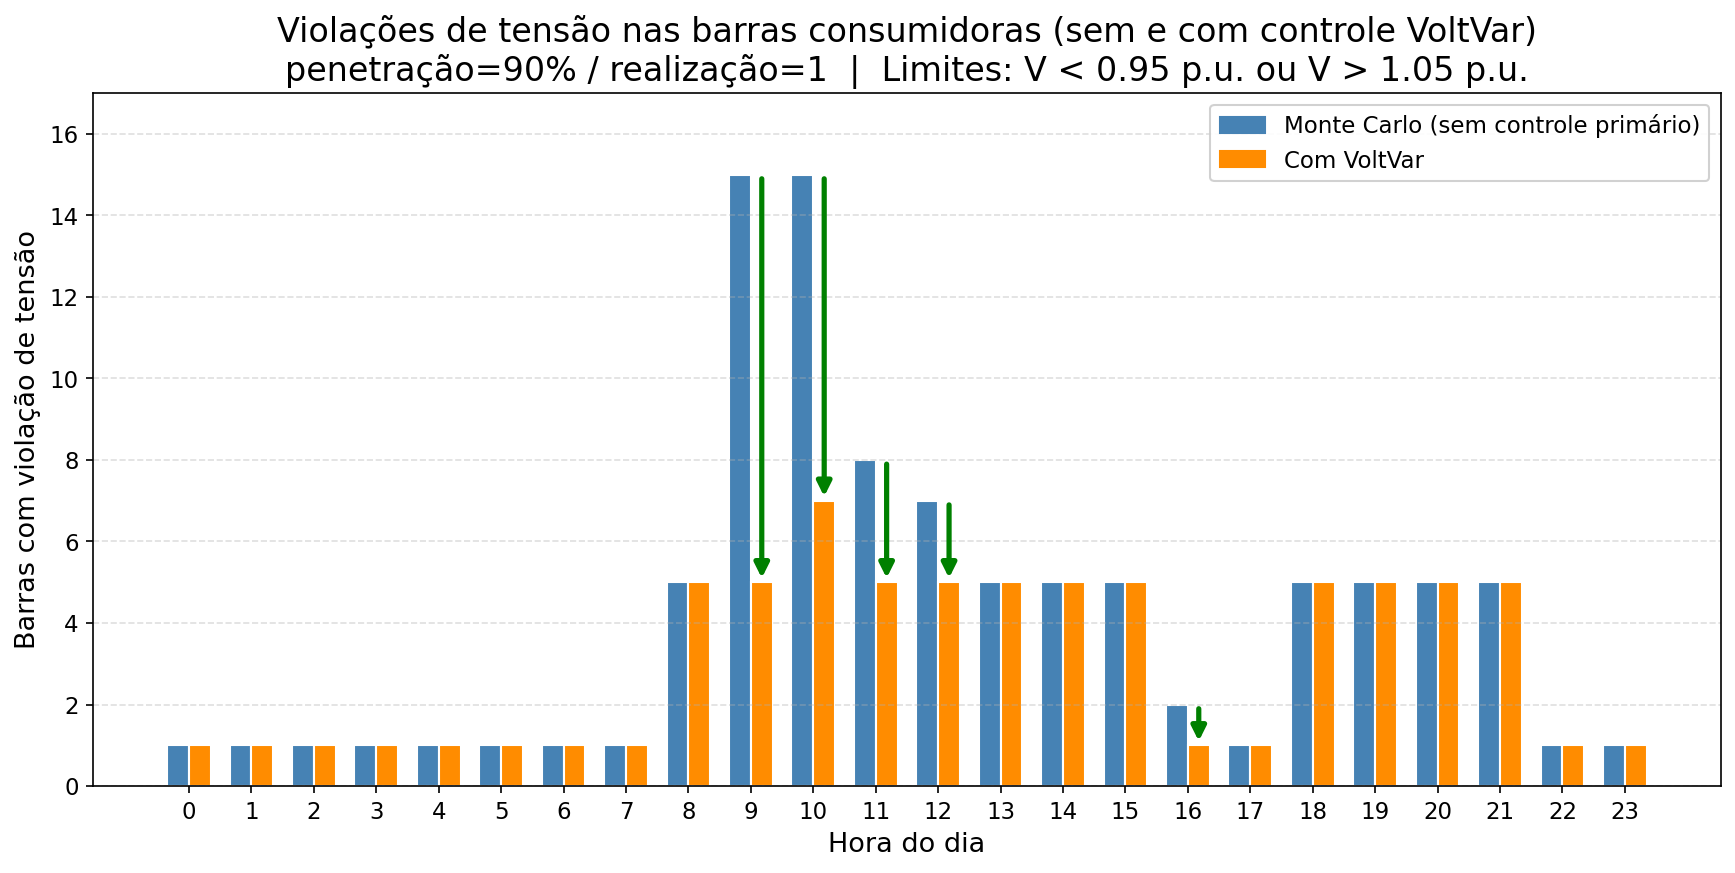
\includegraphics[width=0.8\textwidth]{prim_violations_consumer.png}
  \par\vspace{2pt}\fonte{autoria própria}
\end{figure}

A Figura~\ref{fig:prim_qativacao} apresenta o mapa de ativação do controle, com o valor de $Q/Q_\text{max}$ resultante para cada RED ao longo do dia. O controle é ativado principalmente durante o pico de geração fotovoltaica (horas 8--16), com absorção de reativos para conter sobretensões na maioria das barras. A exceção é a barra~890, que apresenta subtensão estrutural devido à elevada impedância do alimentador lateral que a serve e, por isso, recebe injeção de reativos. Como a estratégia calcula a potência reativa a partir da potência ativa instantânea, não há corte de potência ativa: a regulação ocorre apenas pela alteração do fator de potência, o que constitui uma vantagem operacional.

\begin{figure}[!htb]
  \centering
  \caption{Mapa de ativação do controle primário ($Q/Q_\text{max}$ por RED e por hora).}
  \label{fig:prim_qativacao}
  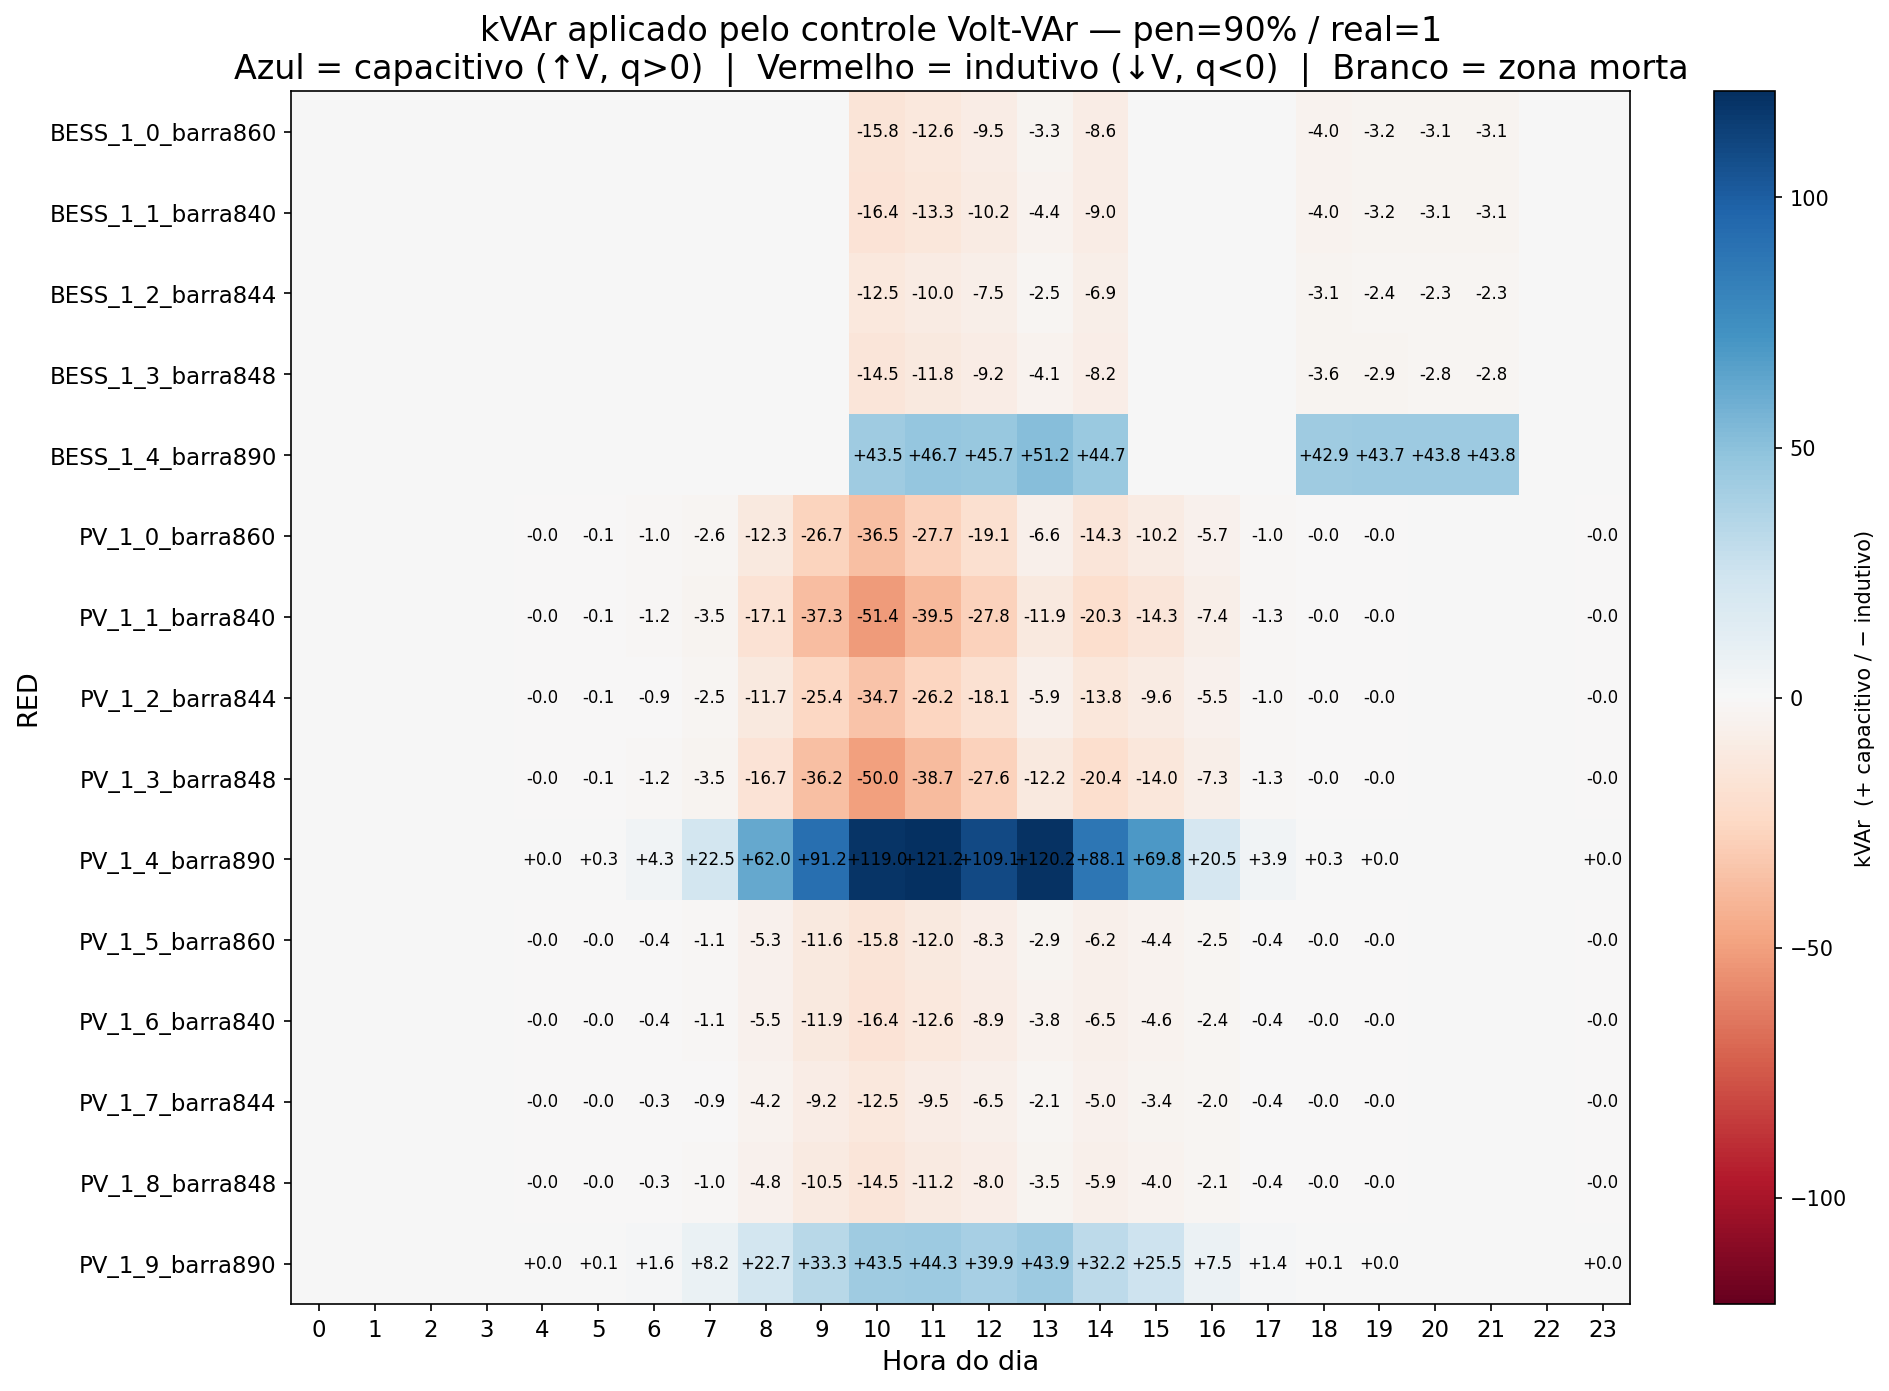
\includegraphics[width=0.8\textwidth]{prim_q_activation.png}
  \par\vspace{2pt}\fonte{autoria própria}
\end{figure}

A Figura~\ref{fig:prim_vmax} apresenta a tensão máxima entre as fases de cada barra ao longo do dia, já com o controle ativo. Persistem dois comportamentos residuais: a barra~890 permanece em subtensão estrutural durante todo o dia, com mínimo de aproximadamente 0,85~p.u. próximo à hora~10; e as barras de cabeceira do alimentador (802, 806, 808 e 810) excedem 1,05~p.u. durante o pico de geração, evidenciando que a absorção local de reativos não elimina todas as sobretensões. Esses resultados residuais reforçam a necessidade da camada de controle secundário.

\begin{figure}[!htb]
  \centering
  \caption{Tensão máxima entre as fases por barra ao longo do dia, com controle primário ativo.}
  \label{fig:prim_vmax}
  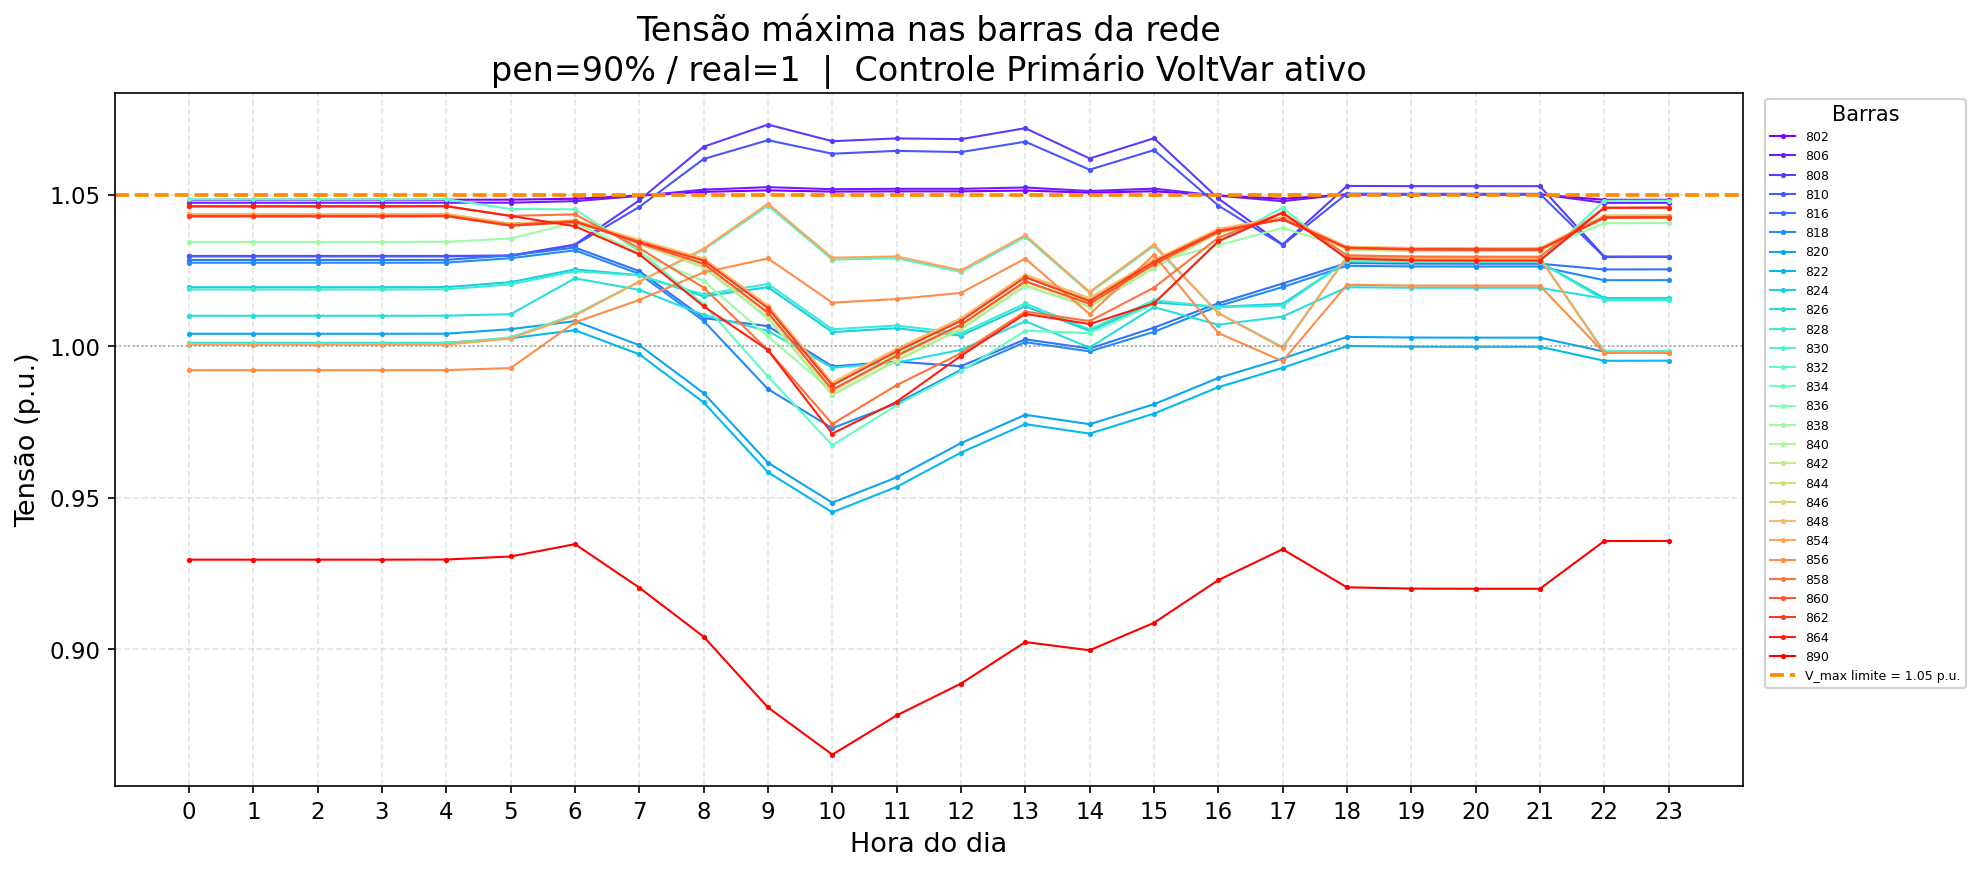
\includegraphics[width=0.8\textwidth]{prim_vmax.png}
  \par\vspace{2pt}\fonte{autoria própria}
\end{figure}

\section{Validação em cenário único: controle duplo}
\label{sec:res_secundario}

Sobre o mesmo cenário, avaliou-se a atuação do controle secundário por consenso como camada complementar ao primário. A Figura~\ref{fig:sec_violations} compara o número de barras com violação nos três casos: sem controle, com primário isolado e com primário e secundário. O efeito predominante do secundário é corretivo nas horas 18 a 21, período de descarga programada dos BESS e de pico de demanda noturna, em que o número de barras violadas cai de cinco (apenas com o primário) para quatro. Entretanto, observa-se um efeito adverso pontual nas horas 11 e 13, em que o número de barras violadas aumenta de cinco para sete. Esse comportamento decorre da própria natureza da parcela de consenso Laplaciana, que redistribui potência ativa entre os BESS para equalizar seus estados de carregamento, podendo introduzir desequilíbrios de tensão pontuais em barras que, sob a ação isolada do primário, encontravam-se dentro dos limites.

\begin{figure}[!htb]
  \centering
  \caption{Barras com violação de tensão por hora: sem controle, com primário isolado e com primário e secundário (cenário de 90\% de penetração).}
  \label{fig:sec_violations}
  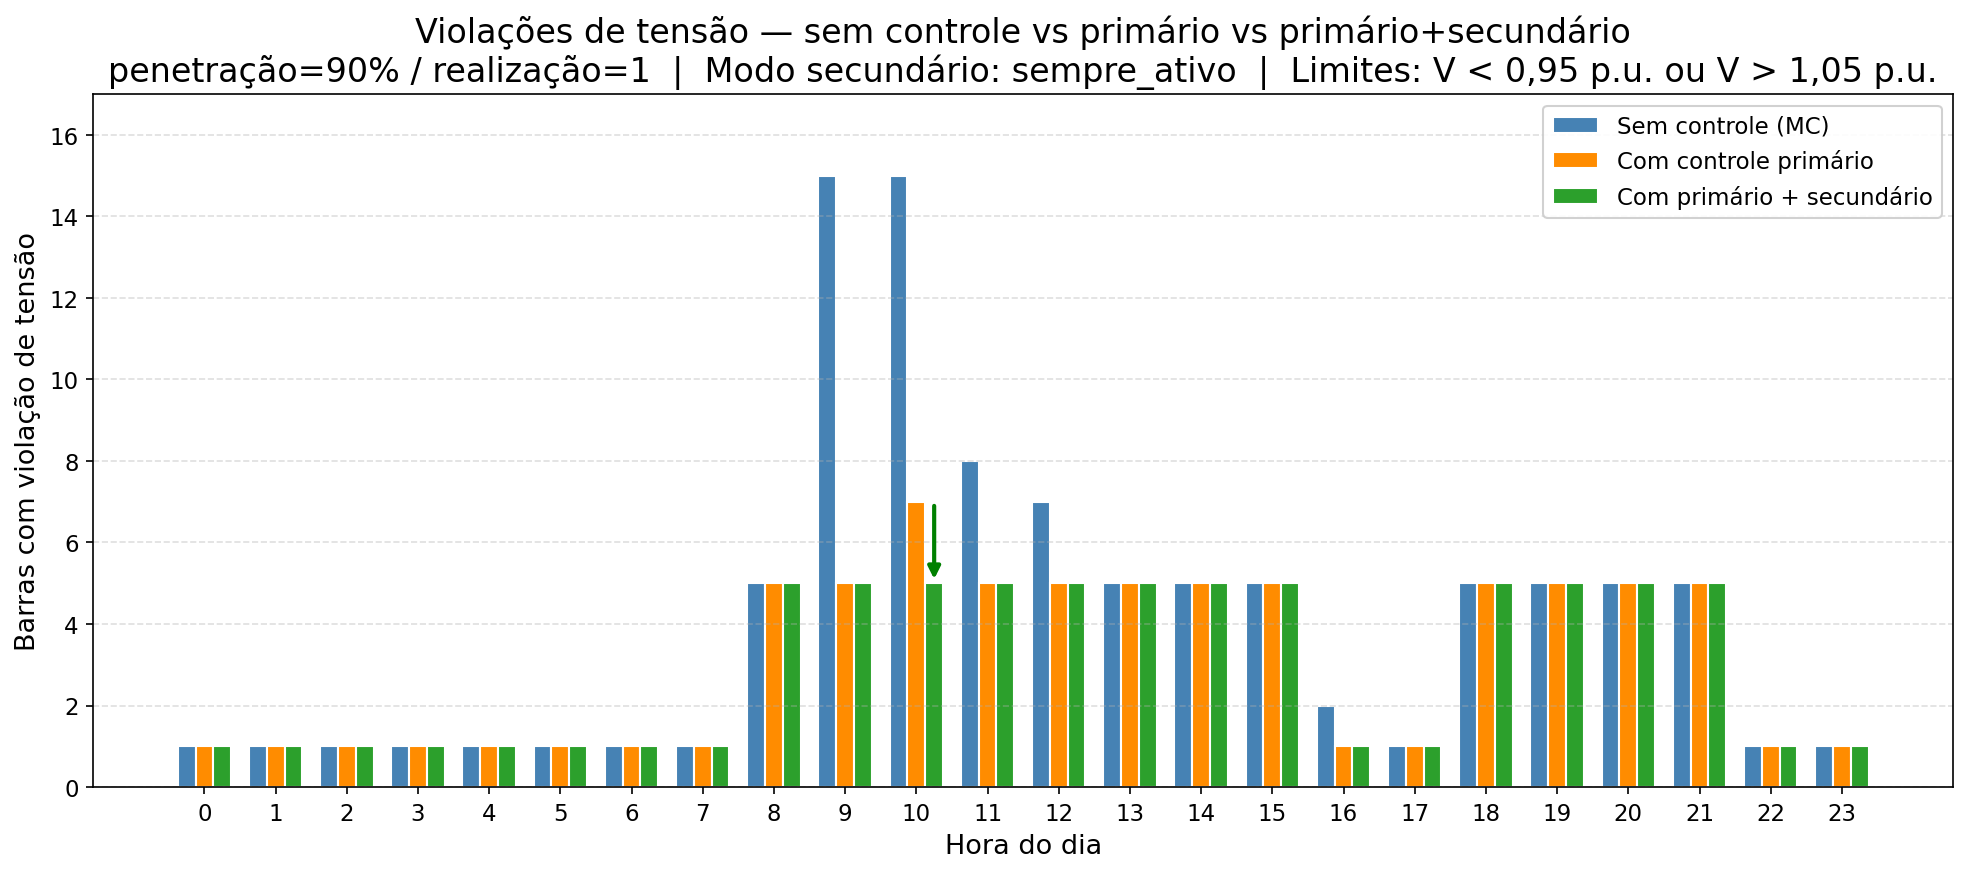
\includegraphics[width=0.8\textwidth]{sec_violations_3way.png}
  \par\vspace{2pt}\fonte{autoria própria}
\end{figure}

A Figura~\ref{fig:sec_bess_kw} compara, para cada BESS, o perfil de potência ativa de referência com o efetivamente aplicado após o consenso. Os BESS das barras 860, 840 e 844 apresentam desvios pequenos, de modo que o consenso praticamente preserva o despacho original; em contraste, os das barras 848 e, sobretudo, 890 apresentam desvios acentuados, com a unidade da barra~890 chegando a inverter sua operação em parte da janela diurna. Esse comportamento, detalhado pelo mapa de correções da Figura~\ref{fig:sec_deltap}, é coerente com a subtensão estrutural da barra~890: o consenso concentra nela a maior parte da correção. Ainda assim, a tensão mínima dessa barra (cerca de 0,876~p.u. na hora~9) permanece próxima à obtida apenas com o primário, indicando que a elevada impedância do alimentador lateral continua limitando a eficácia da regulação nesse ponto específico.

\begin{figure}[!htb]
  \centering
  \caption{Perfil de potência ativa dos BESS: referência \emph{versus} pós-consenso (cenário de 90\% de penetração).}
  \label{fig:sec_bess_kw}
  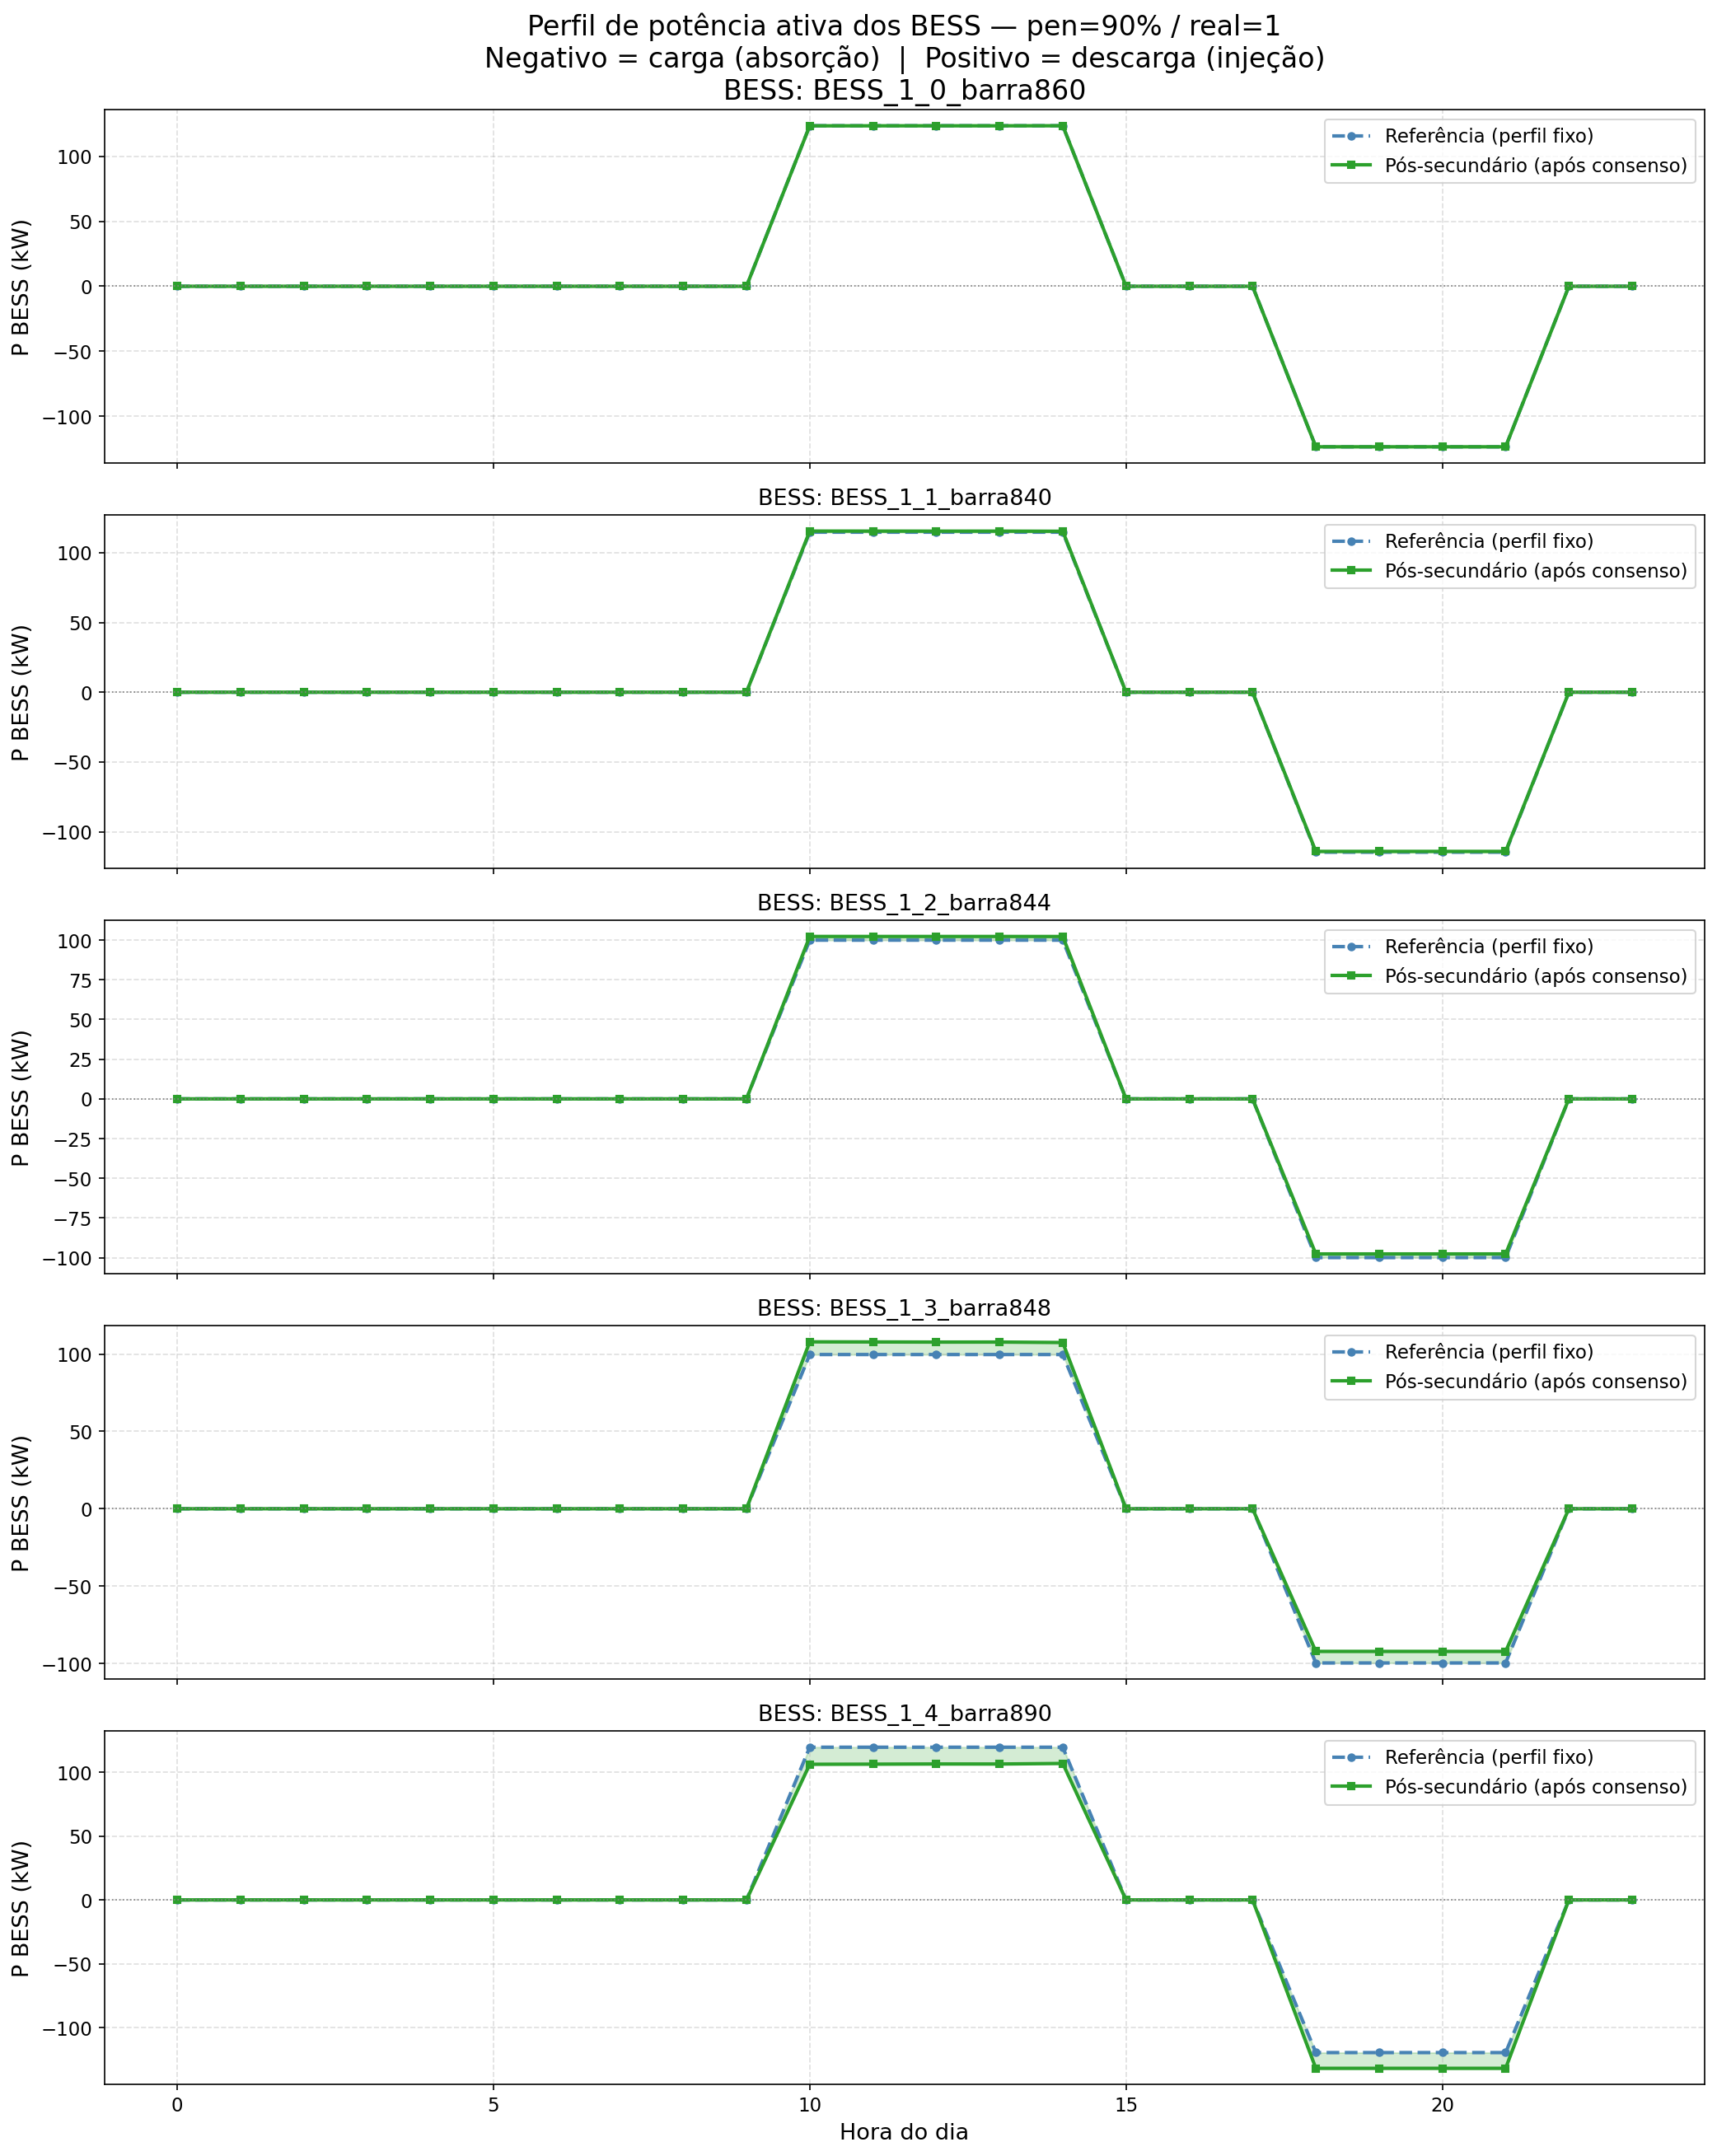
\includegraphics[width=0.8\textwidth]{sec_bess_kw_profile.png}
  \par\vspace{2pt}\fonte{autoria própria}
\end{figure}

\begin{figure}[!htb]
  \centering
  \caption{Mapa das correções de potência ativa ($\Delta P$) impostas pelo controle secundário por barra e por hora.}
  \label{fig:sec_deltap}
  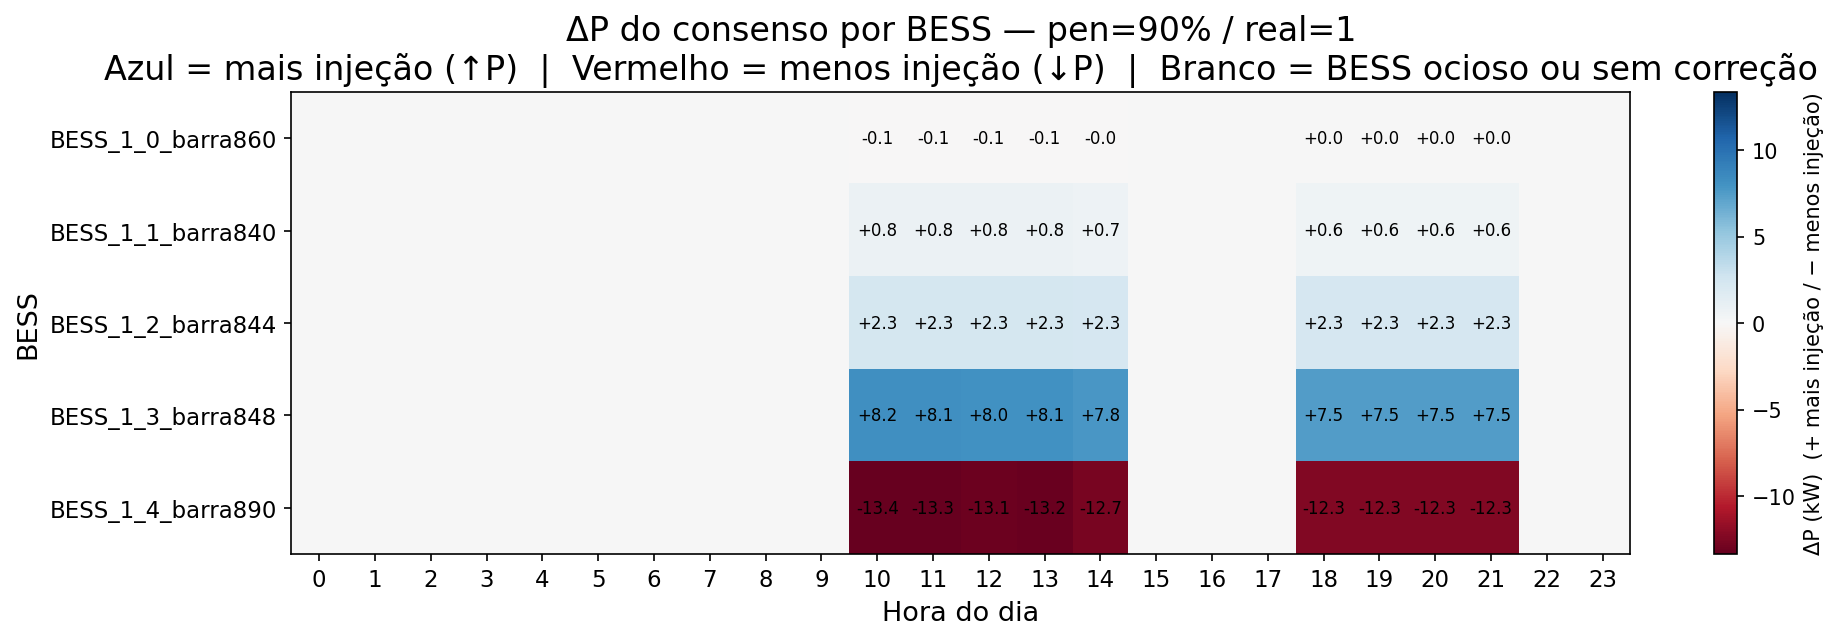
\includegraphics[width=0.8\textwidth]{sec_bess_delta_p_heatmap.png}
  \par\vspace{2pt}\fonte{autoria própria}
\end{figure}

A limitação espacial observada é coerente com a propriedade de soma nula da parcela Laplaciana: como a sobretensão nas horas centrais decorre de um excesso de geração distribuído ao longo do alimentador, e os BESS não estão instalados nas barras de cabeceira, a redistribuição de potência entre unidades tem alcance limitado para corrigir violações em barras eletricamente distantes dos pontos de instalação dos BESS.

\section{Análise probabilística por Monte Carlo}
\label{sec:res_montecarlo}

A avaliação foi então estendida a todos os 5500~cenários, confrontando de forma pareada os três casos. As subseções seguintes caracterizam, primeiro, o caso de referência e, em seguida, o efeito de cada camada de controle.

\subsection{Caso de referência}
\label{sec:res_base}

Os resultados do caso base permitem três constatações. Primeiro, a subtensão não constitui o desafio dominante nesta rede: em todos os níveis de penetração e faixas horárias, o número de barras com subtensão permanece próximo de zero, à exceção da barra~890, cuja subtensão estrutural independe do nível de penetração. Os reguladores automáticos e os bancos de capacitores já mitigam de forma satisfatória os problemas de subtensão.

Segundo, a sobretensão provocada pela injeção fotovoltaica é o fenômeno dominante e cresce sistematicamente com o nível de penetração, como mostra a curva-mestre da Figura~\ref{fig:mc_base}. O comportamento é mais enfático nas barras próximas à subestação e, para dias de céu aberto, o limiar crítico situa-se entre 20\% e 30\% de penetração, acima do qual a probabilidade de violação deixa de ser desprezível. Em alta penetração, a rede satura: nas faixas diurnas, a mediana do número de barras em violação chega a cerca de 20 barras em 100\% de penetração. A Figura~\ref{fig:mc_heatmap_base} localiza esse fenômeno no espaço e no tempo, evidenciando que, em 100\%, a sobretensão deixa de ser localizada nas barras próximas à subestação e passa a comprometer extensões significativas do alimentador.

\begin{figure}[!htb]
  \centering
  \caption{Sobretensão no caso base: média e desvio padrão do número de barras com violação por nível de penetração.}
  \label{fig:mc_base}
  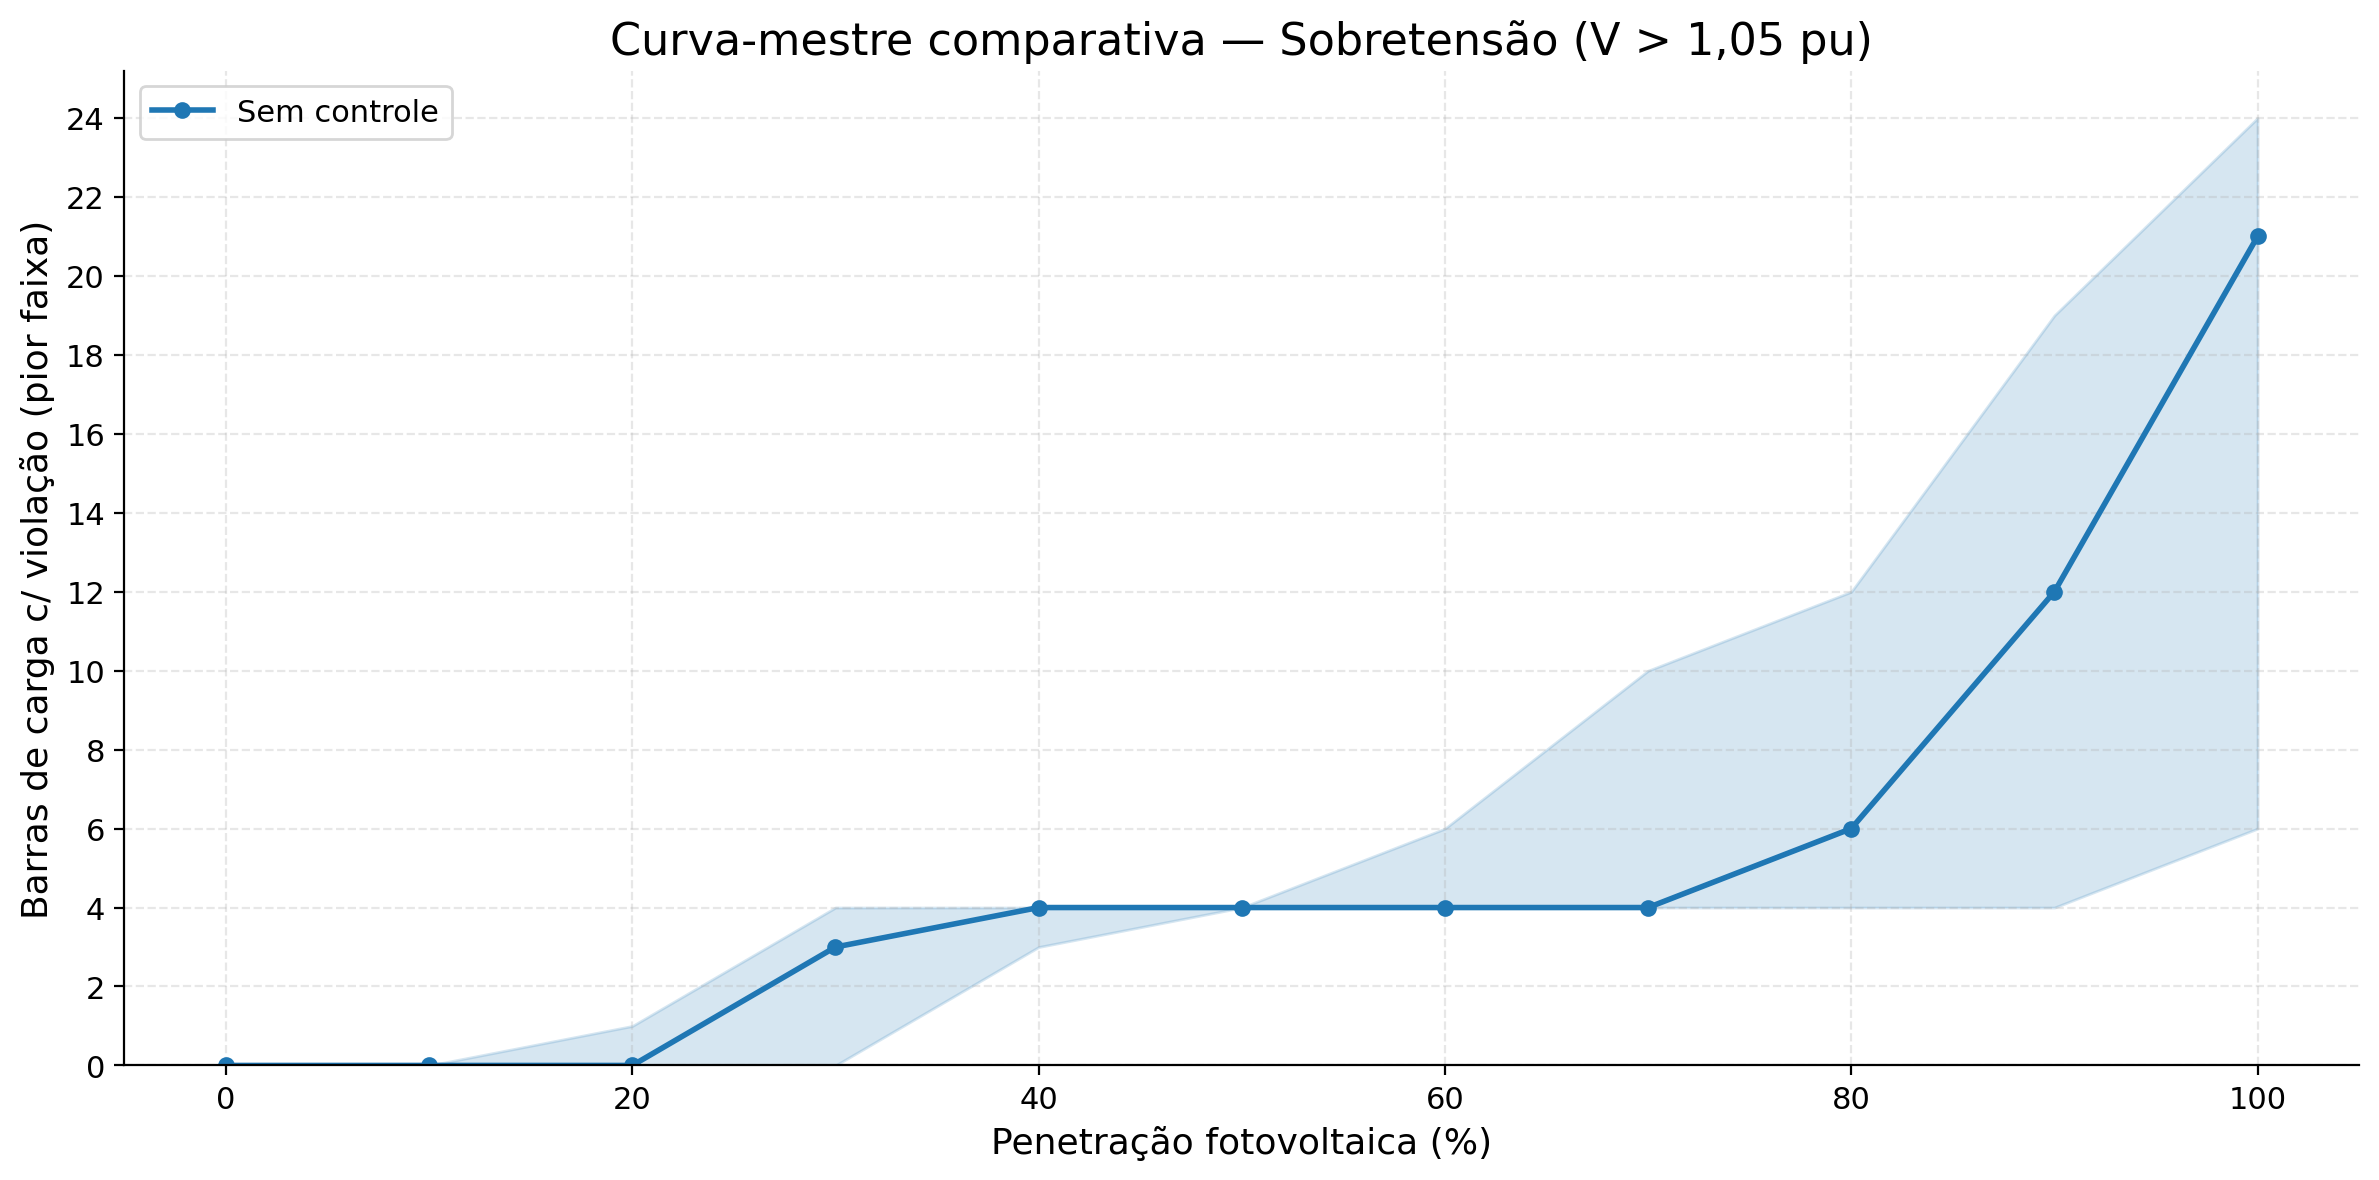
\includegraphics[width=0.78\textwidth]{mc_curva_mestre_base.png}
  \par\vspace{2pt}\fonte{autoria própria}
\end{figure}

\begin{figure}[!htb]
  \centering
  \caption{Probabilidade de sobretensão por barra e hora no caso sem controle, para 100\% de penetração fotovoltaica.}
  \label{fig:mc_heatmap_base}
  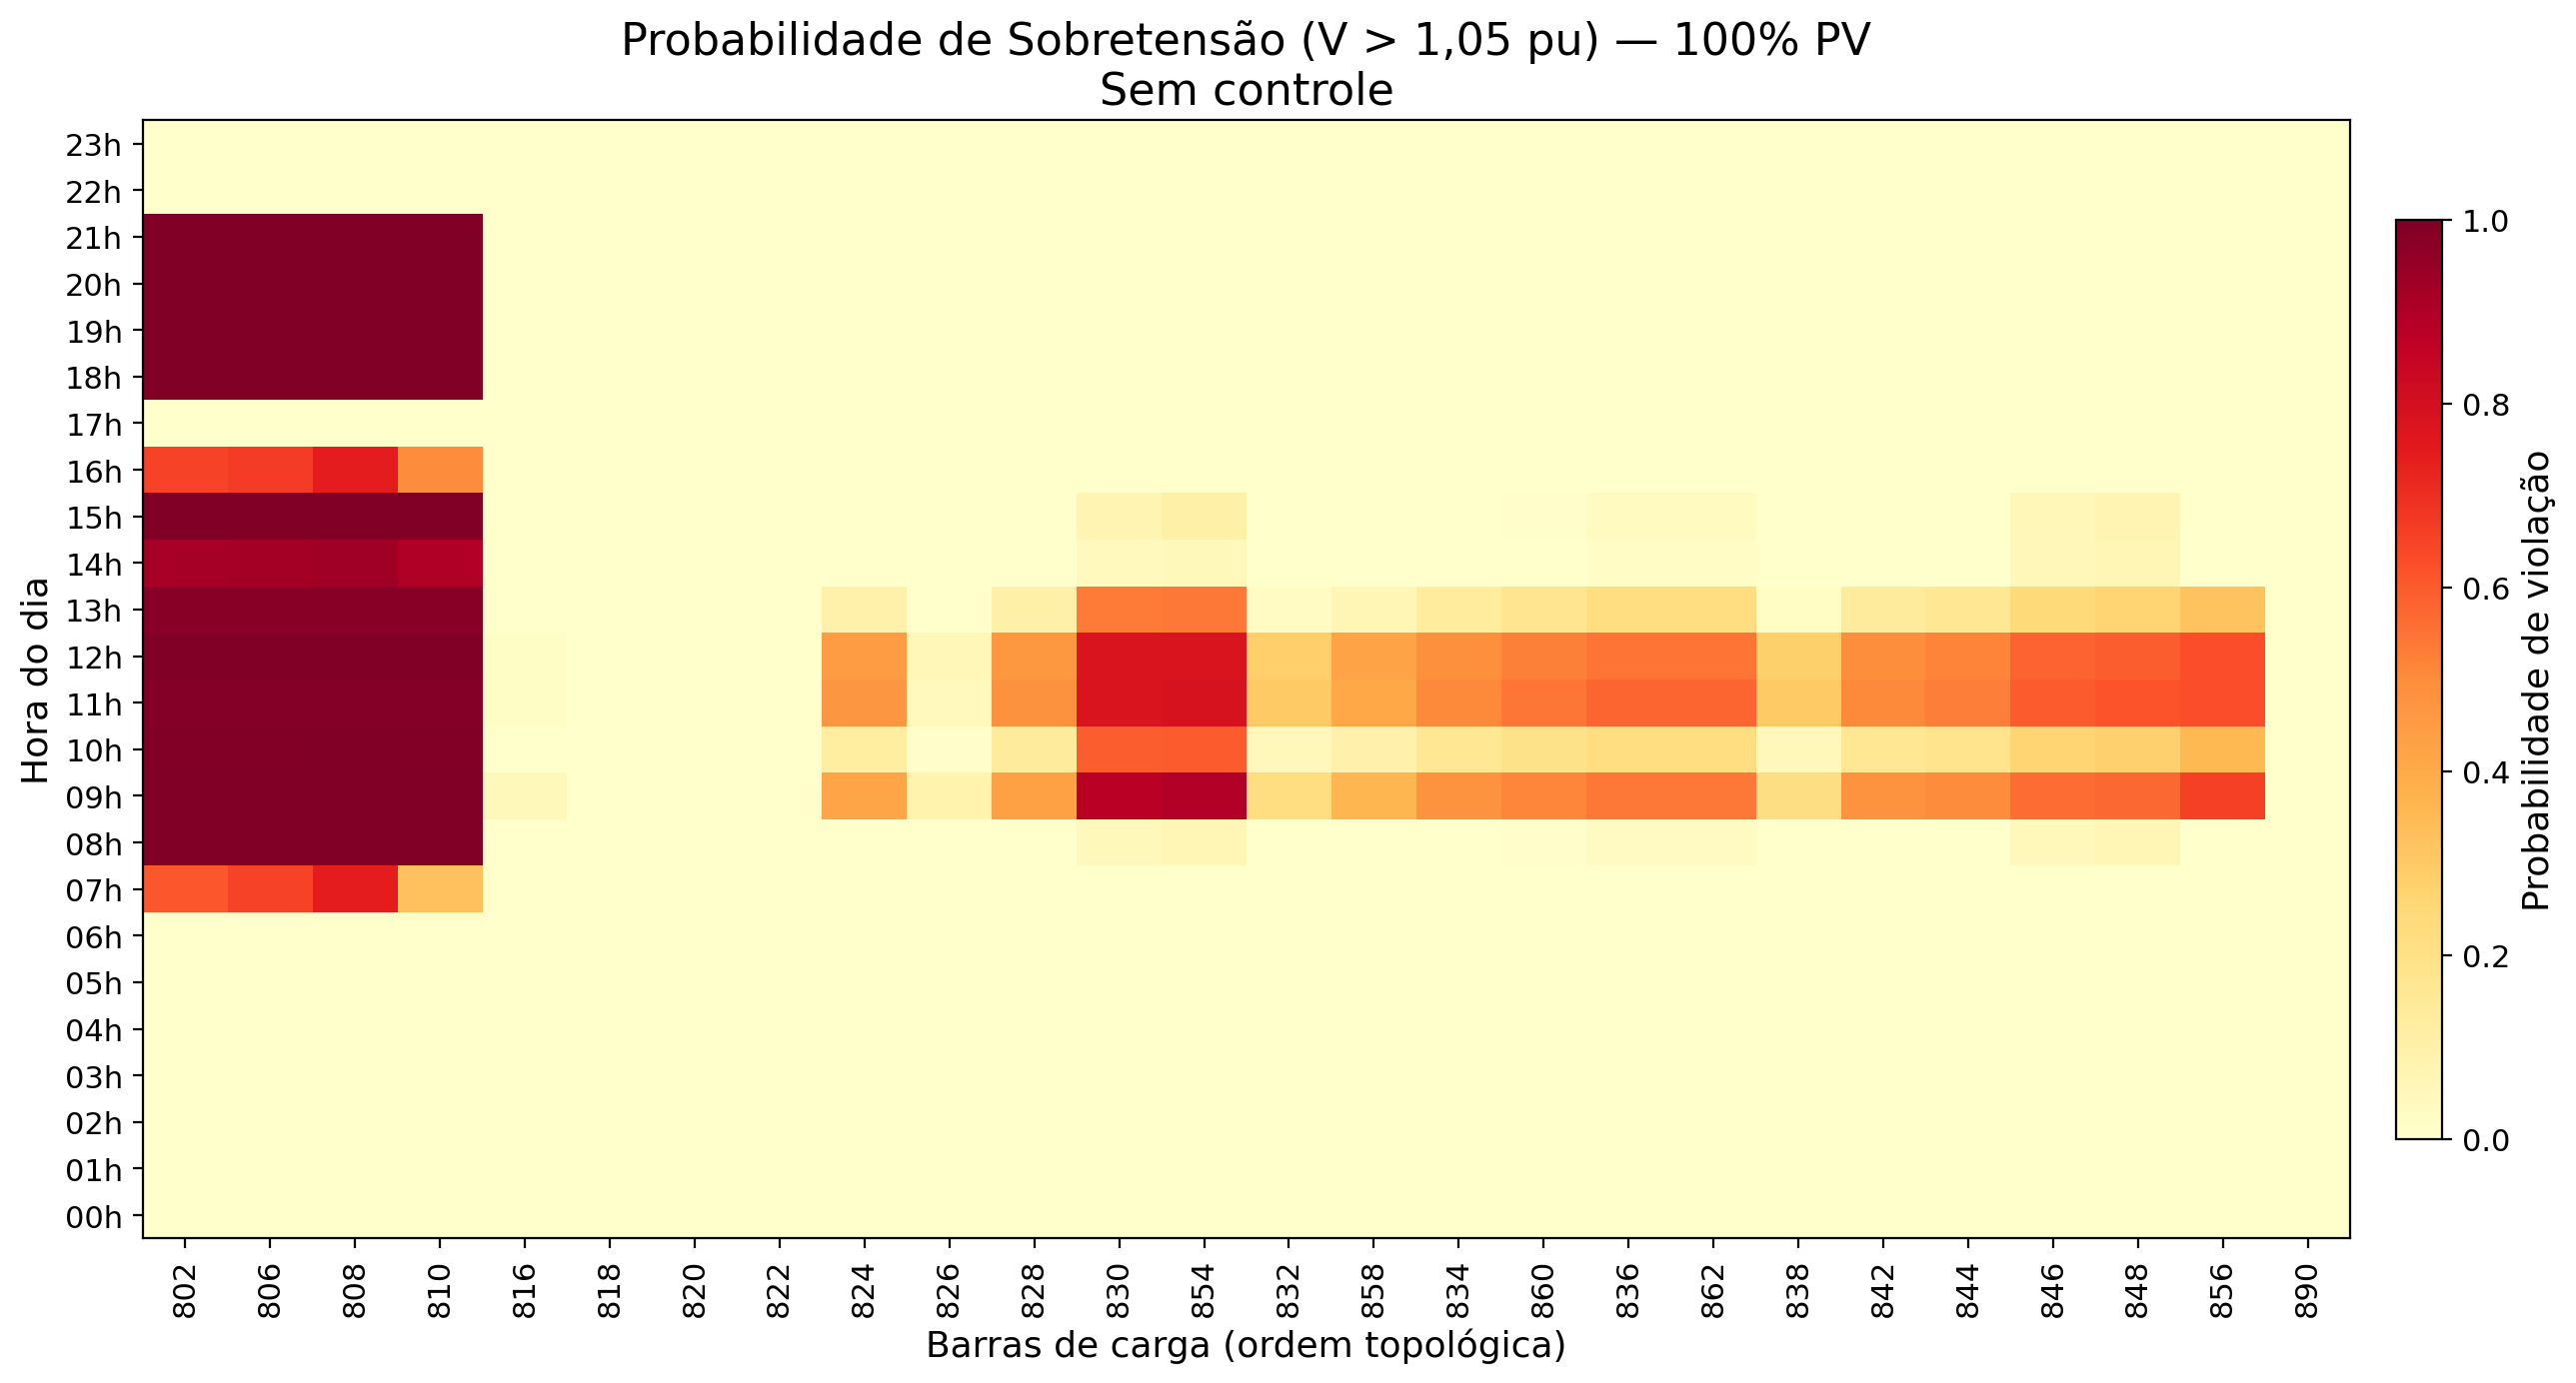
\includegraphics[width=0.78\textwidth]{mc_heatmap_base_100.png}
  \par\vspace{2pt}\fonte{autoria própria}
\end{figure}

Terceiro, o BESS no regime de operação fixo adotado atenua a sobretensão durante o carregamento e contribui para o suporte de tensão noturno, mas sua eficácia é limitada para penetrações acima de 70\%, evidenciando que a simples presença de armazenamento, sem controle otimizado, é insuficiente em cenários de alta penetração.

\subsection{Efeito do controle primário}
\label{sec:res_mc_primario}

Confrontados de forma pareada o caso de referência e o controle primário, este se mostrou eficaz na contenção da sobretensão diurna. A Figura~\ref{fig:mc_barras_primario} apresenta a média e o desvio padrão do número de barras afetadas por nível de penetração: enquanto o caso sem controle atinge média de cerca de dezessete barras em 100\% de penetração, com desvio padrão elevado, o cenário com controle primário estabiliza-se em torno de quatro barras, com dispersão reduzida. O controle não apenas reduz a média, como também comprime a faixa de incerteza entre cenários, tornando o desempenho da rede mais previsível.

\begin{figure}[!htb]
  \centering
  \caption{Sobretensão por nível de penetração: comparação entre o caso sem controle e o controle primário (todos os tipos de dia).}
  \label{fig:mc_barras_primario}
  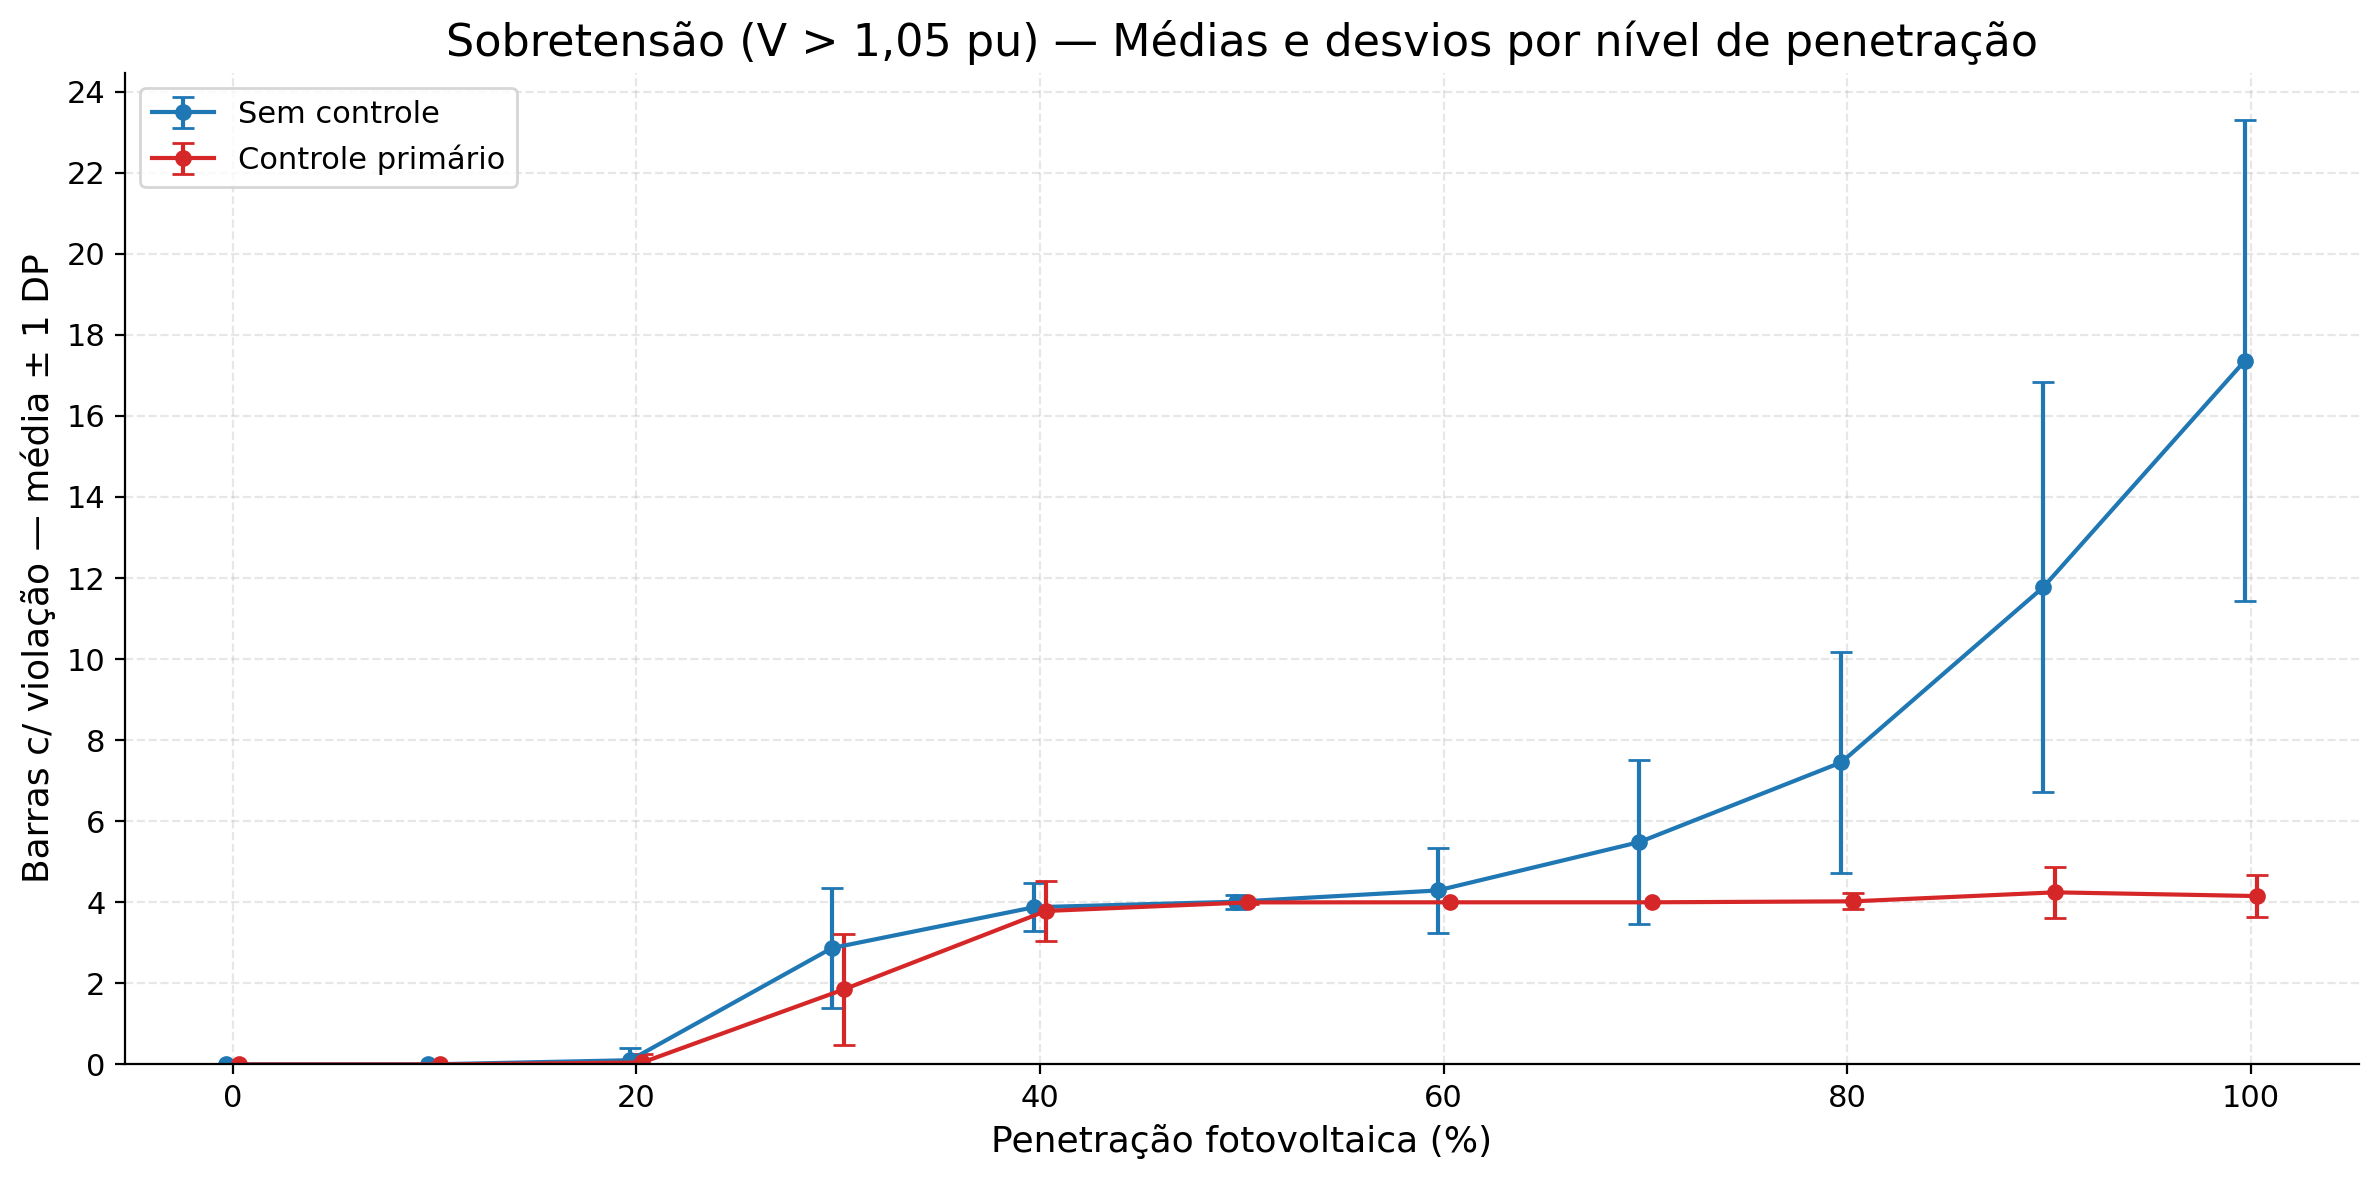
\includegraphics[width=0.78\textwidth]{mc_barras_erro_primario.png}
  \par\vspace{2pt}\fonte{autoria própria}
\end{figure}

O detalhamento horário, na Figura~\ref{fig:mc_boxplot_primario}, mostra que, em 100\% de penetração, o número de barras em violação dispara nas horas centrais do dia no caso de referência, com medianas entre 12 e 15 barras, enquanto o cenário com controle primário se mantém estável em torno de quatro barras ao longo de toda a janela diurna. O mapa de diferença de probabilidade da Figura~\ref{fig:mc_heatmap_dif} isola o efeito do controle: os valores positivos indicam redução da probabilidade de violação, e a ausência de valores negativos confirma que o controle primário não agrava a sobretensão em nenhuma barra ou horário, atuando de forma seletiva e mais intensa precisamente onde e quando a sobretensão é mais provável.

\begin{figure}[!htb]
  \centering
  \caption{Distribuição horária do número de barras com sobretensão para 100\% de penetração: sem controle \emph{versus} controle primário.}
  \label{fig:mc_boxplot_primario}
  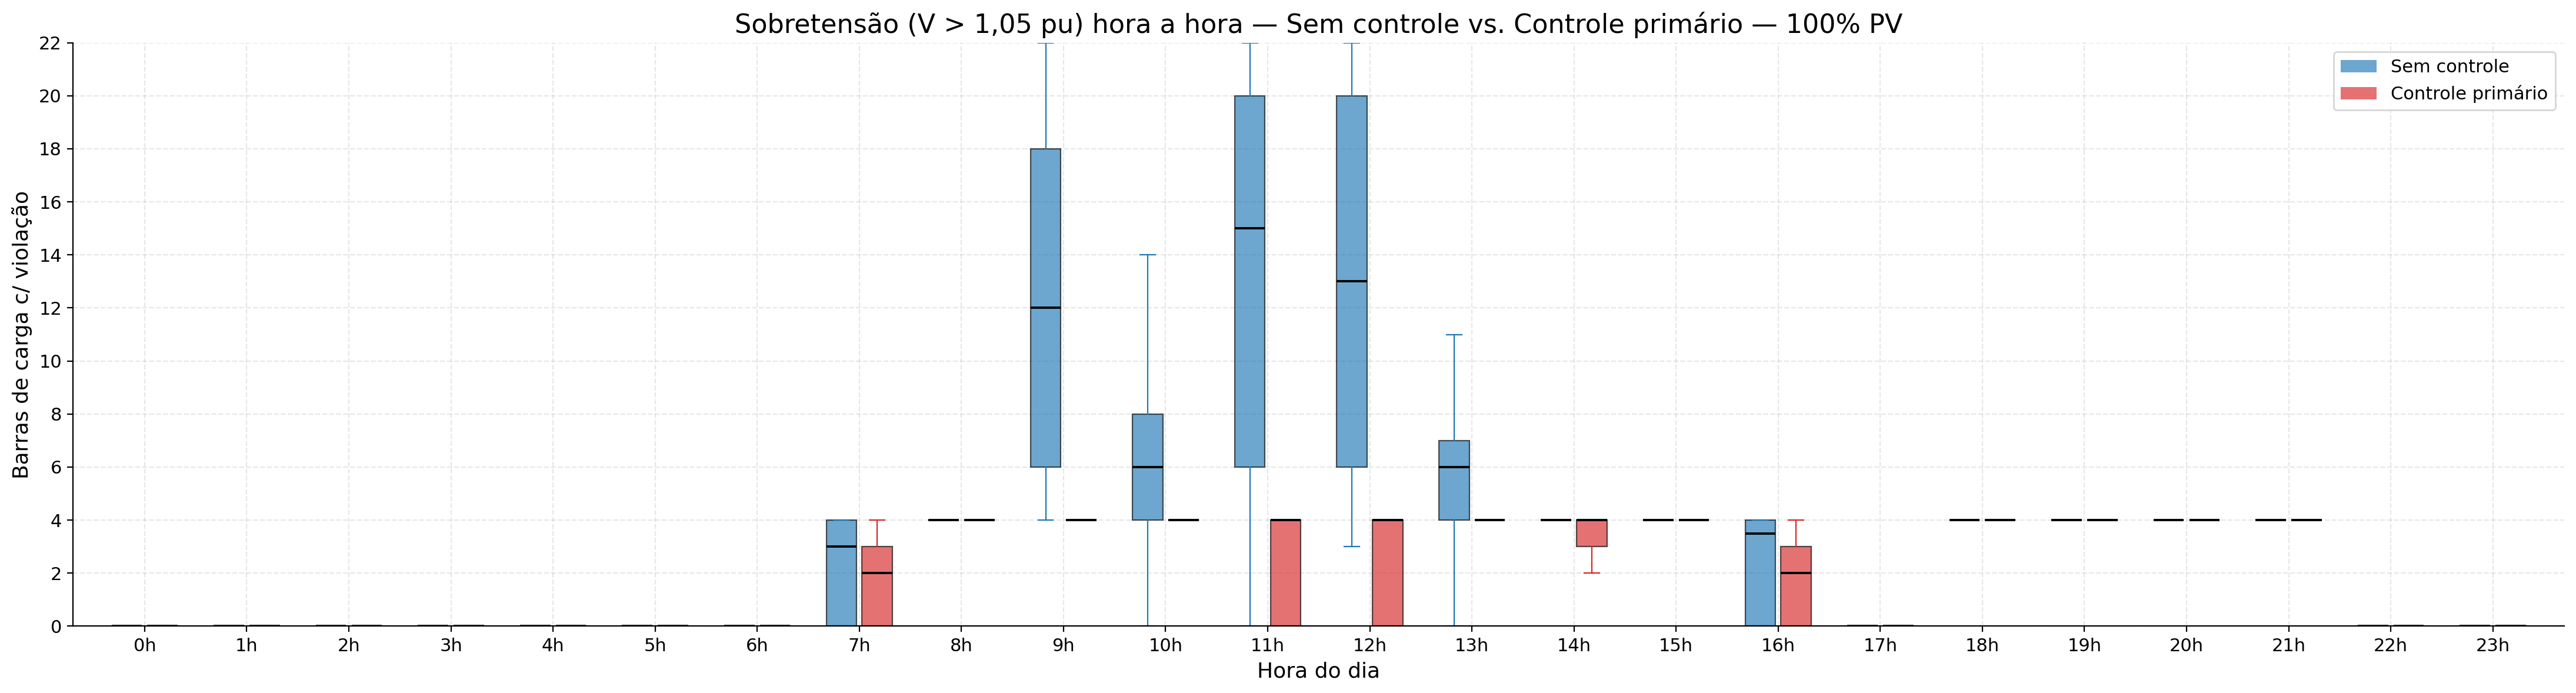
\includegraphics[width=0.78\textwidth]{mc_boxplot_primario_100.png}
  \par\vspace{2pt}\fonte{autoria própria}
\end{figure}

\begin{figure}[!htb]
  \centering
  \caption{Diferença de probabilidade de sobretensão (sem controle $-$ controle primário) por barra e hora, para 100\% de penetração.}
  \label{fig:mc_heatmap_dif}
  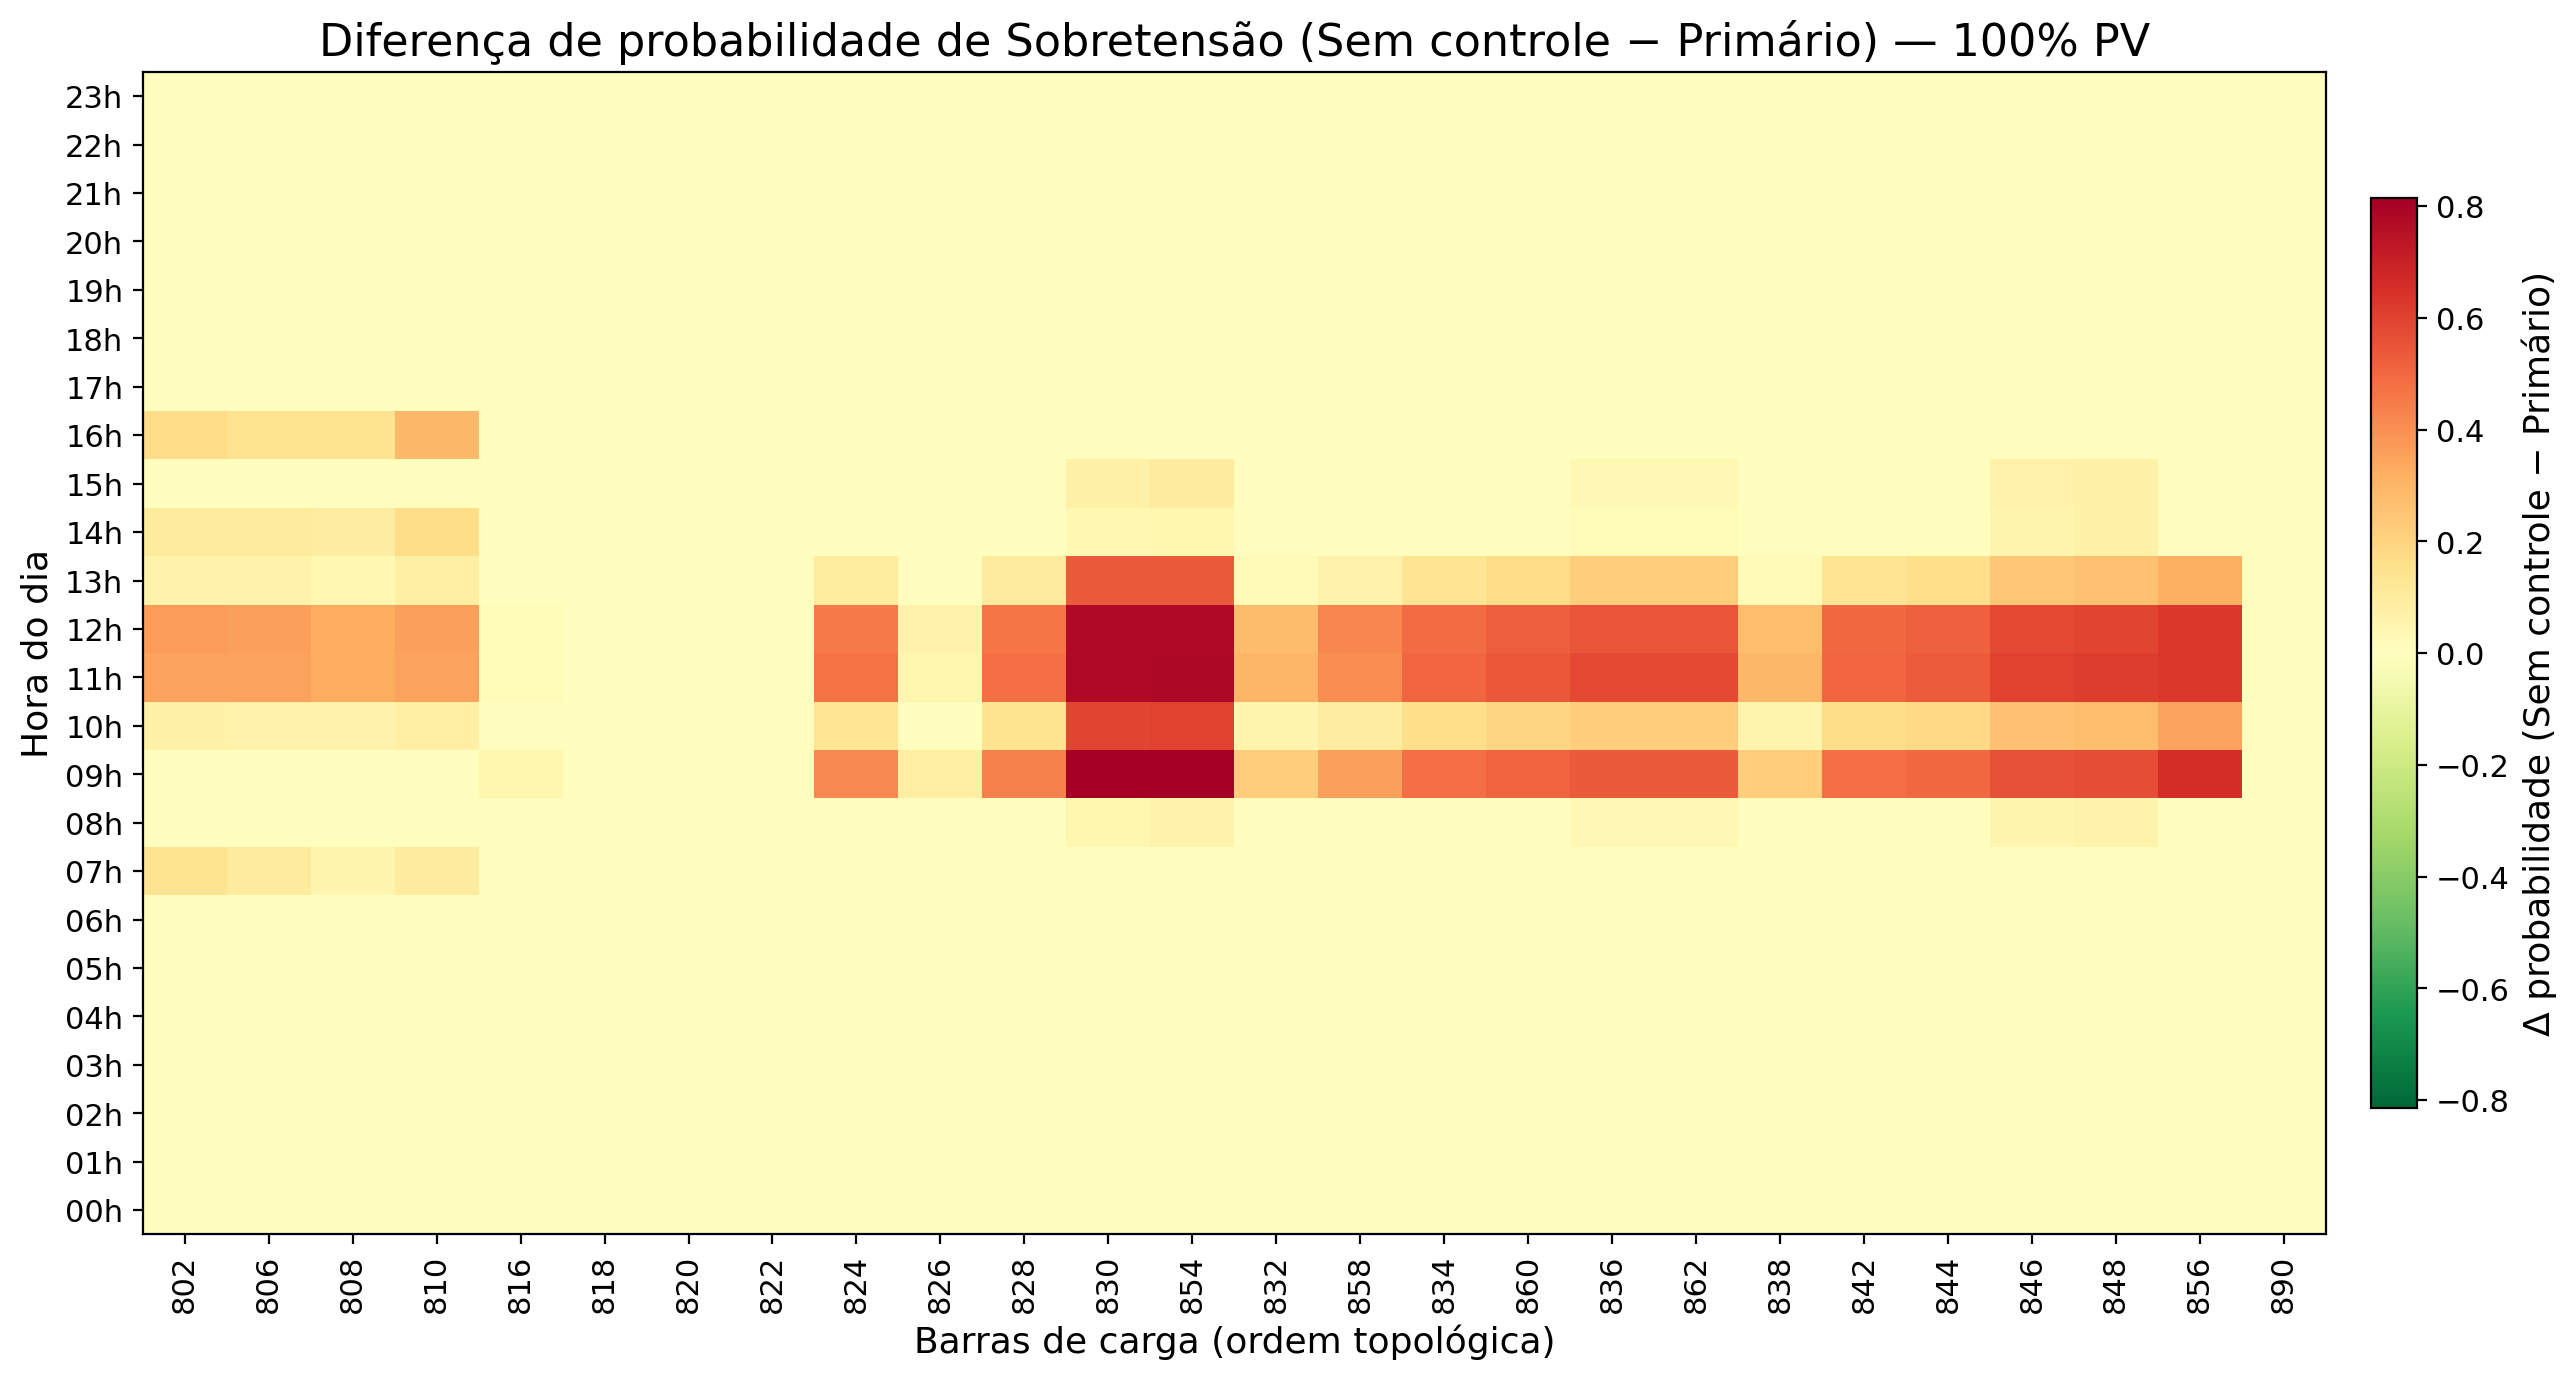
\includegraphics[width=0.78\textwidth]{mc_heatmap_dif_primario_100.png}
  \par\vspace{2pt}\fonte{autoria própria}
\end{figure}

\subsection{Efeito do controle duplo por consenso}
\label{sec:res_mc_duplo}

O controle duplo foi avaliado com o secundário atuando condicionalmente ao primário, isto é, apenas nas horas em que ainda restam violações após a ação do controle primário. A Figura~\ref{fig:mc_tres} sintetiza os três casos. Diferentemente do esperado, o controle duplo \emph{não} cumpriu o objetivo de reduzir as violações de sobretensão remanescentes ao primário. Ao contrário, para os níveis de 90\% e 100\% de penetração observou-se uma mediana de cerca de duas barras a mais em violação do que no caso com apenas controle primário, além de efetividade altamente variável, oscilando entre 2 e 12 barras em violação para 100\% de penetração.

\begin{figure}[!htb]
  \centering
  \caption{Curva-mestre comparativa da sobretensão para os três casos: sem controle, controle primário e controle duplo.}
  \label{fig:mc_tres}
  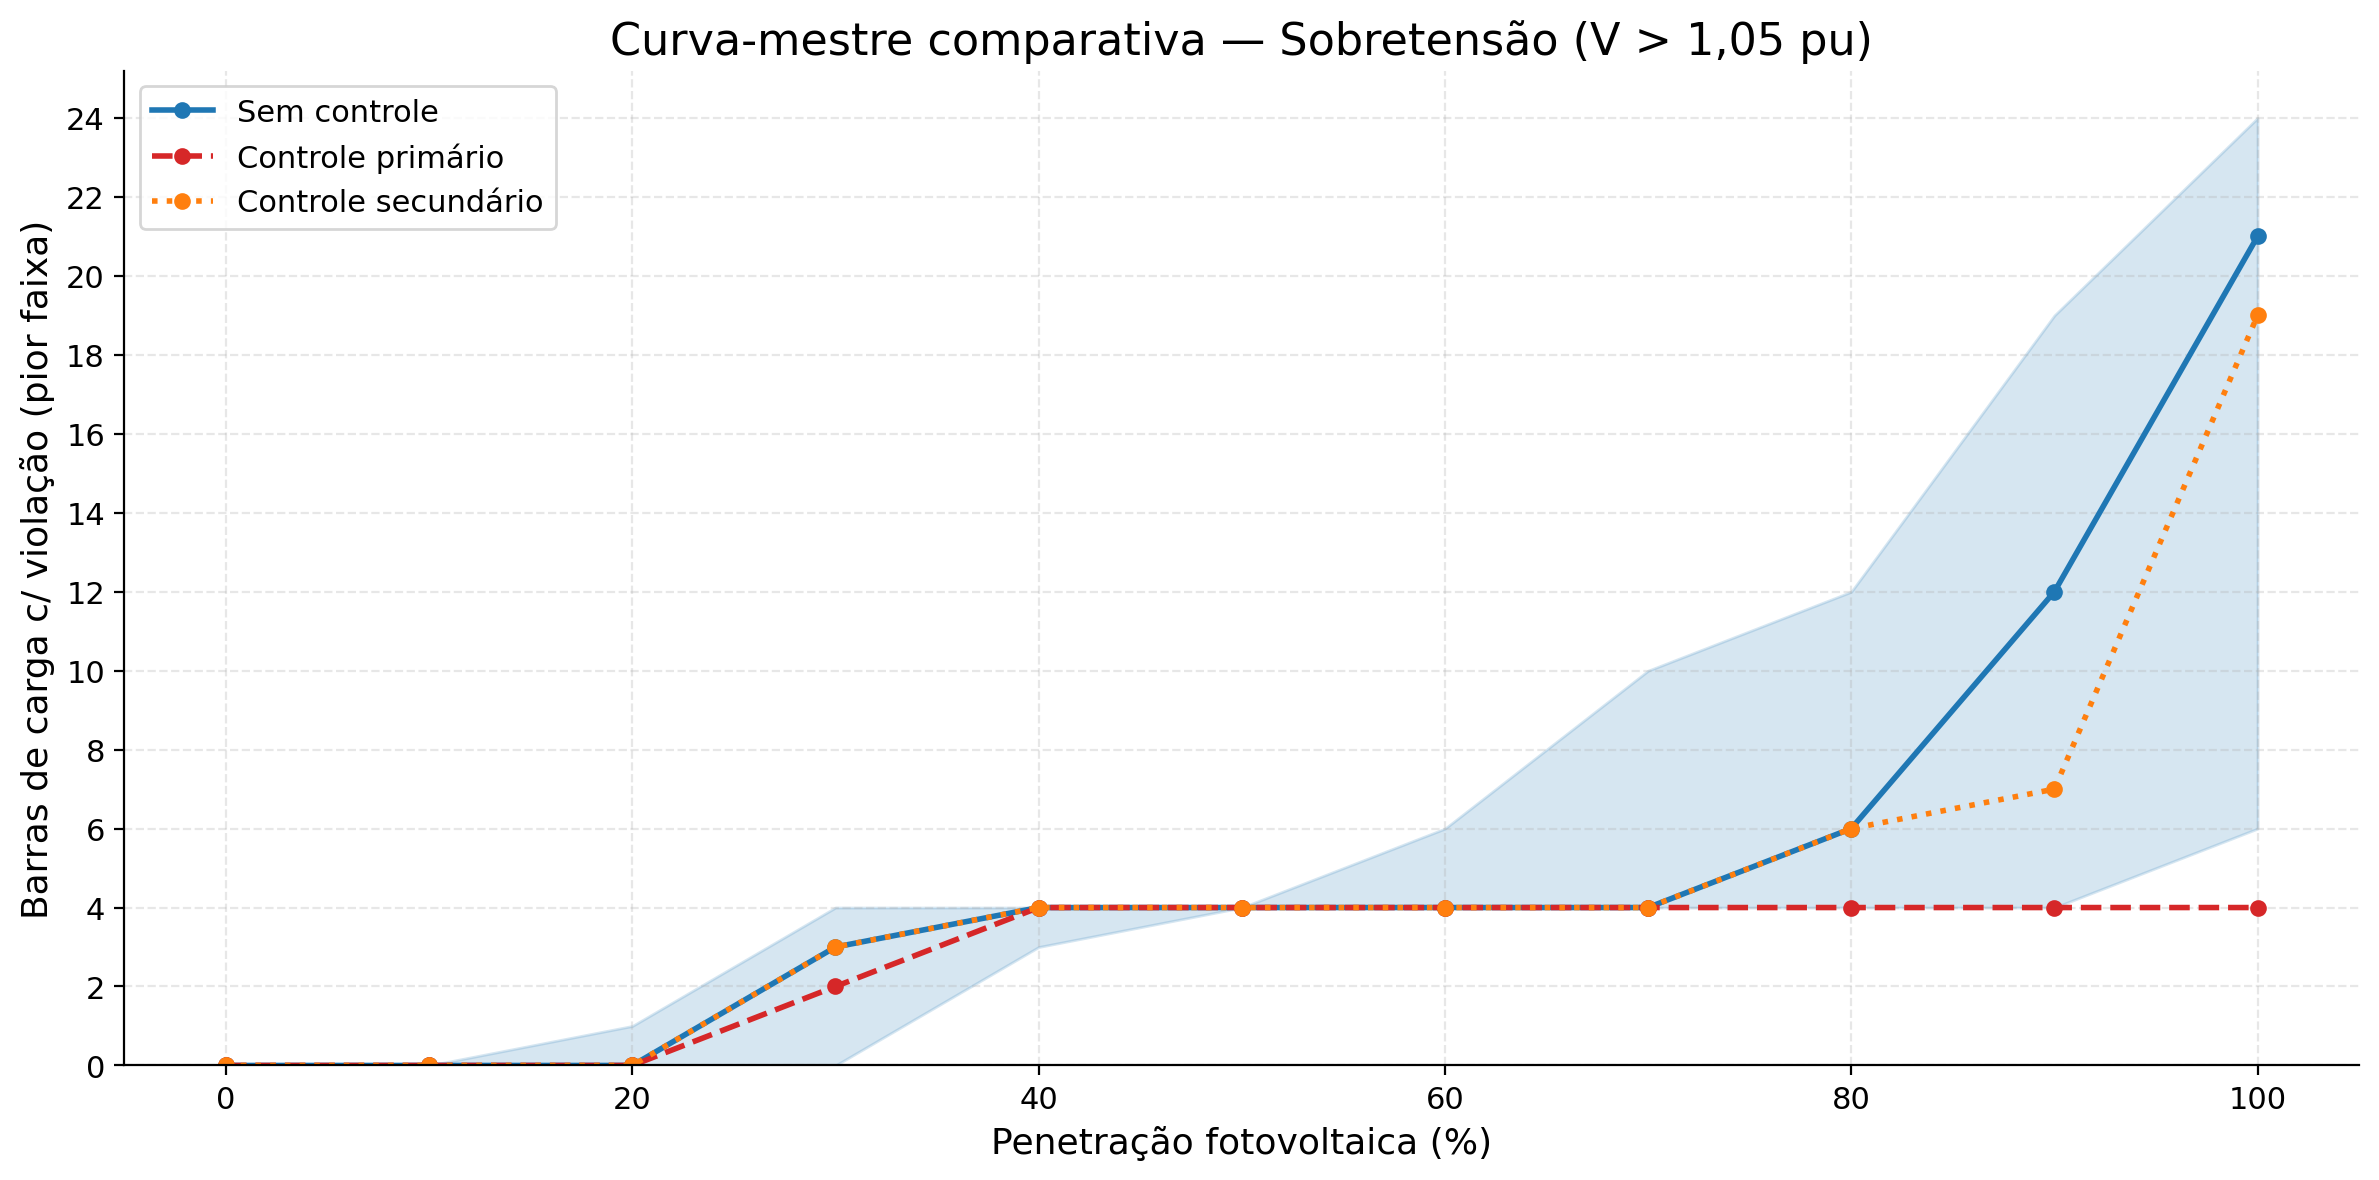
\includegraphics[width=0.78\textwidth]{mc_curva_mestre_tres.png}
  \par\vspace{2pt}\fonte{autoria própria}
\end{figure}

O não funcionamento do controle duplo nas condições estudadas decorre da concentração dos BESS em uma região específica do alimentador, o que limita seu efeito sobre as barras próximas à subestação --- justamente as mais críticas em alta penetração ---, conforme já discutido na análise do cenário único (Seção~\ref{sec:res_secundario}). Esse resultado, embora negativo, é informativo: delimita as condições de eficácia da camada de consenso e aponta que sua aplicação depende fortemente da alocação espacial do armazenamento em relação às barras críticas. As implicações para os próximos passos do projeto são discutidas no Capítulo~\ref{cap:conclusao}.

\chapter{Conclusão}
\label{cap:conclusao}

Este relatório documentou a primeira etapa do Projeto de Formatura, dedicada ao desenvolvimento 
e à avaliação de uma estratégia de controle distribuído em dupla camada para BESS, voltada à 
regulação de tensão em redes de distribuição de média tensão com alta penetração de geração 
fotovoltaica. A seguir, retomam-se os objetivos específicos definidos na 
Seção~\ref{sec:objetivos}, confrontando-os com os resultados obtidos.

A revisão da literatura (Capítulo~\ref{cap:fundamentacao}) sistematizou as arquiteturas de 
controle e as principais formulações distribuídas, identificando os algoritmos de consenso 
como a base predominante da camada de coordenação e fundamentando as escolhas metodológicas 
do trabalho. O ambiente de cossimulação Python--OpenDSS (Capítulo~\ref{cap:ambiente}) foi 
desenvolvido e validado na rede IEEE~33 barras, estabelecendo a infraestrutura para a execução 
de fluxos de potência iterativos em séries temporais. A geração de cenários por Monte Carlo 
(Capítulo~\ref{cap:cenarios}) produziu um conjunto de 5500~cenários sobre a rede IEEE~34 
barras, contemplando onze níveis de penetração e a incerteza de irradiância, alocação de 
recursos e demanda. As duas camadas de controle (Capítulo~\ref{cap:controle}) foram 
implementadas e integradas, e seu desempenho foi avaliado de forma pareada 
(Capítulo~\ref{cap:resultados}).

Quanto à avaliação de desempenho, três conclusões se destacam. Primeiro, nas condições 
simuladas, o desafio dominante de regulação de tensão é a sobretensão diurna, que cresce 
sistematicamente com a penetração fotovoltaica, enquanto a subtensão é satisfatoriamente 
mitigada pelos dispositivos convencionais da rede, à exceção da barra de extremidade do 
ramal de 4,16~kV. Segundo, o controle primário por curva volt-var mostrou-se eficaz: 
reduziu de forma expressiva o número médio de barras em sobretensão (de cerca de dezessete 
para quatro em 100\% de penetração) e comprimiu a dispersão entre cenários, tornando o 
desempenho da rede mais previsível, sem causar corte de geração. Terceiro, o controle 
secundário por consenso, na rede e configuração estudadas, não reduziu as violações 
remanescentes ao primário, apresentando inclusive efeito adverso pontual; tal resultado 
decorre da concentração espacial dos BESS no alimentador, que limita o alcance da 
redistribuição de potência sobre as barras críticas próximas à subestação.

O resultado negativo da camada de consenso, longe de invalidar a abordagem, delimita suas 
condições de eficácia e orienta os próximos passos. Cabe ressaltar dois ajustes em relação ao 
plano de trabalho, ambos justificados ao longo do texto: a adoção da biblioteca 
OpenDSSDirect.py em lugar da interface COM, e a substituição da lógica \emph{fuzzy} pela curva 
volt-var normatizada, estendida também aos inversores FV.

\section{Trabalhos futuros}
\label{sec:futuro}

Os resultados obtidos delineiam os próximos passos da pesquisa, a serem desenvolvidos na 
segunda etapa do Projeto de Formatura:

\begin{itemize}
  \item aprimorar os modelos de FV e BESS, em particular incorporando o rastreamento do estado de carga (SoC) das baterias, hoje modeladas como elementos de carga equivalente;
  \item reavaliar o desempenho da rede na ausência dos reguladores automáticos de tensão, isolando a contribuição do controle distribuído;
  \item revisar a alocação e o dimensionamento do armazenamento, incluindo mais unidades ou uma rede mais favorável, de modo a criar condições adequadas à atuação da camada de consenso, e definir novos critérios de desempenho, como redução de perdas, suporte de reativos e mitigação de desequilíbrio;
  \item estender a solução a redes trifásicas desequilibradas, analisando o impacto da assimetria de fases sobre o algoritmo de controle;
  \item incorporar modelos de degradação e ciclo de vida das baterias ao laço de controle; e
  \item aplicar a metodologia a uma rede de distribuição real, aproximando a avaliação das condições operacionais efetivas.
\end{itemize}


% ========== Referências ==========
% Colchetes nos rótulos da lista (ex.: [1], [2]), preservando a estrutura do abntex2cite
\makeatletter
\renewcommand{\@biblabel}[1]{[{\citenumstyle #1}]\hspace{\biblabelsep}}
\makeatother
\bibliographystyle{abntex2-num}
\bibliography{referencias}

% ========== Apêndices ==========
\apendice
\chapter{Resultados do fluxo de potência na rede IEEE~33 barras}
\label{ap:fluxo33}

Este apêndice apresenta os resultados detalhados da simulação de validação do ambiente, descrita na Seção~\ref{sec:ieee33}, para a rede IEEE~33 barras operando em modo \emph{snapshot} a 100\% da carga nominal. A Tabela~\ref{tab:tensoes33} apresenta as tensões nodais em valores por unidade. Observa-se o perfil decrescente ao longo do alimentador, com a barra~18 atingindo a menor tensão (0,9059~p.u.); ao todo, 20~barras operam abaixo do limite de 0,95~p.u.

\begin{table}[!htb]
  \centering
  \caption{Tensões nodais na rede IEEE~33 barras (tensão de base de 7,309~kV em todas as barras).}
  \label{tab:tensoes33}
  \footnotesize
  \begin{tabular}{@{}cc@{\hspace{1.5cm}}cc@{}}
    \toprule
    \textbf{Barra} & \textbf{$V$ (p.u.)} & \textbf{Barra} & \textbf{$V$ (p.u.)} \\
    \midrule
    B1  & 0,9984 & B18 & 0,9059 \\
    B2  & 0,9954 & B19 & 0,9949 \\
    B3  & 0,9816 & B20 & 0,9913 \\
    B4  & 0,9743 & B21 & 0,9906 \\
    B5  & 0,9671 & B22 & 0,9900 \\
    B6  & 0,9492 & B23 & 0,9780 \\
    B7  & 0,9458 & B24 & 0,9713 \\
    B8  & 0,9327 & B25 & 0,9680 \\
    B9  & 0,9267 & B26 & 0,9473 \\
    B10 & 0,9212 & B27 & 0,9449 \\
    B11 & 0,9204 & B28 & 0,9338 \\
    B12 & 0,9190 & B29 & 0,9259 \\
    B13 & 0,9132 & B30 & 0,9224 \\
    B14 & 0,9110 & B31 & 0,9184 \\
    B15 & 0,9097 & B32 & 0,9176 \\
    B16 & 0,9084 & B33 & 0,9173 \\
    B17 & 0,9065 &     &        \\
    \bottomrule
  \end{tabular}
  \par\vspace{2pt}\fonte{autoria própria}
\end{table}

A corrente mais elevada ocorre na linha 1--2, que drena toda a demanda da rede (206,99~A; 1284,39~kW de potência ativa). As correntes diminuem progressivamente ao longo do alimentador à medida que as cargas são atendidas. A tabela completa de correntes e fluxos de potência por linha está disponível no repositório do projeto~\cite{repositorio}.

\chapter{Fluxogramas dos algoritmos e da arquitetura computacional}
\label{ap:fluxogramas}

Este apêndice reúne os fluxogramas das implementações computacionais descritas nos Capítulos~\ref{cap:controle} e~\ref{cap:resultados}. A Figura~\ref{fig:flux_secundario} apresenta o laço de controle secundário por consenso, contemplando a construção do grafo de comunicação, a verificação do número mínimo de BESS e o laço iterativo de cálculo da variável de consenso, do produto Laplaciano, da parcela de \emph{droop} e dos sinais $\Delta P$ e $\Delta Q$. A Figura~\ref{fig:flux_arquitetura} apresenta a arquitetura computacional modular, evidenciando o fluxo de dados entre a geração de cenários, os motores de simulação de cada estratégia de controle e o pós-processamento estatístico e gráfico. O laço do controle primário, por sua vez, está descrito em detalhe na Seção~\ref{sec:primario}.

\begin{figure}[!htb]
  \centering
  \caption{Fluxograma do controle secundário por consenso.}
  \label{fig:flux_secundario}
  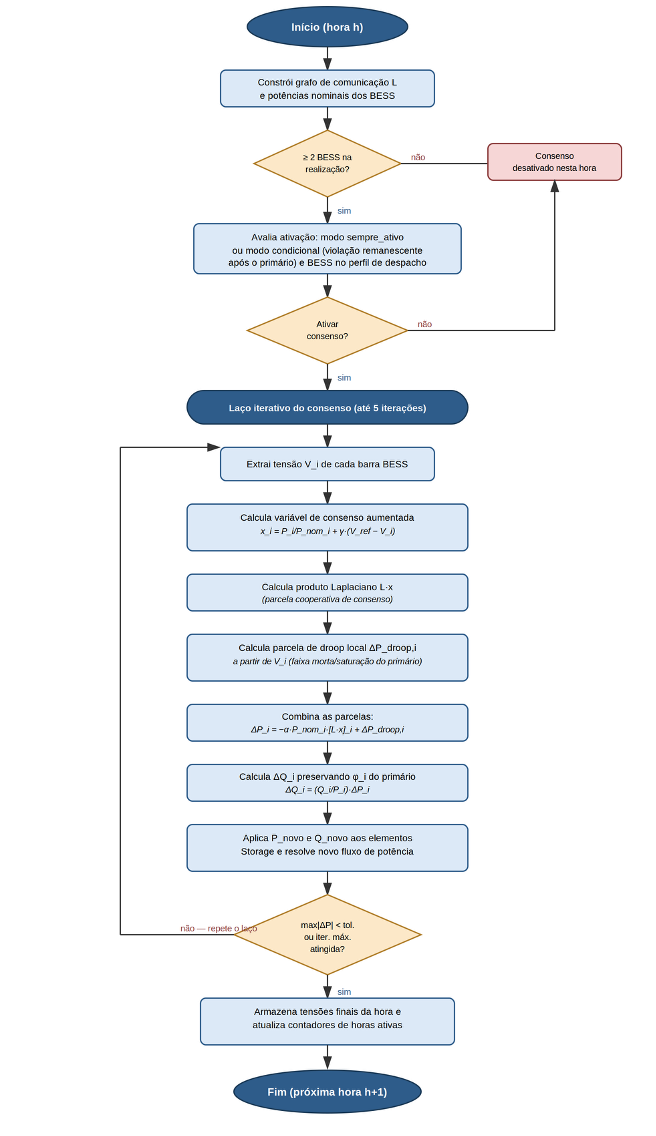
\includegraphics[height=0.82\textheight]{fluxograma-consenso.png}
  \par\vspace{2pt}\fonte{autoria própria}
\end{figure}

\begin{figure}[!htb]
  \centering
  \caption{Arquitetura computacional: blocos principais e fluxo de dados entre a geração de cenários, a simulação sob cada estratégia de controle e o pós-processamento.}
  \label{fig:flux_arquitetura}
  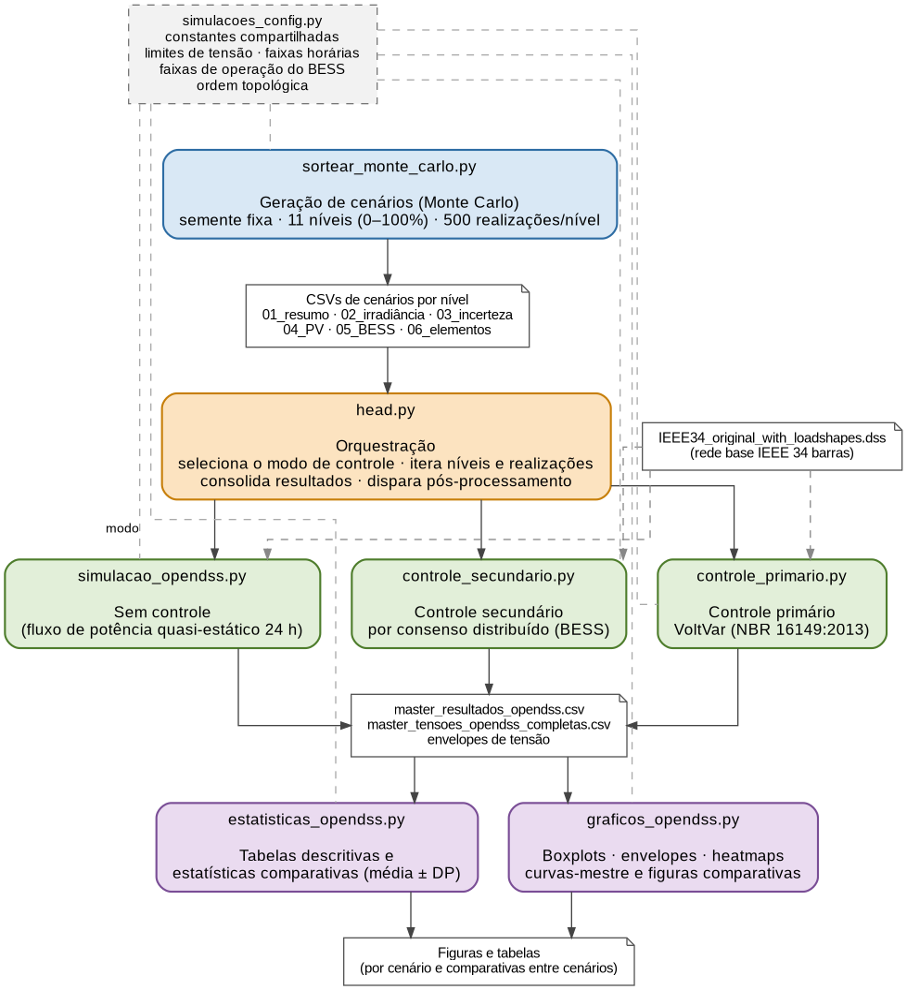
\includegraphics[height=0.82\textheight]{fluxograma-monte_carlo-primario-consenso.png}
  \par\vspace{2pt}\fonte{autoria própria}
\end{figure}


% ========== Anexos ==========
\anexo
\chapter{Dados do alimentador IEEE~34 barras}
\label{an:ieee34}

A rede de estudo deste trabalho é o alimentador de testes \emph{IEEE 34 Bus Test Feeder}, definido pelo \emph{Distribution System Analysis Subcommittee} do IEEE \emph{Power and Energy Society}. Os dados de topologia, condutores, matrizes de impedância de fase (códigos 300 a 304), reguladores de tensão, bancos de capacitores e cargas correspondem à especificação oficial do alimentador, descrita na Seção~\ref{sec:ieee34}. O arquivo de definição da rede no formato \texttt{.dss}, com as adaptações de perfis de carga horária introduzidas neste trabalho, está disponível no repositório do projeto~\cite{repositorio}.

\chapter{Base de dados de irradiância SONDA/INPE}
\label{an:sonda}

Os perfis de irradiância empregados na geração de cenários (Seção~\ref{sec:irradiancia}) baseiam-se em medições do Sistema de Organização Nacional de Dados Ambientais (SONDA), operado pelo Instituto Nacional de Pesquisas Espaciais (INPE)~\cite{inpe_sonda}. Utilizaram-se as séries de irradiância global horizontal da estação de Cachoeira Paulista (SP), referentes ao período de janeiro de 2023 a dezembro de 2025. Os dados originais são de domínio público e estão disponíveis no portal da rede SONDA.

\chapter{Sobretensão no caso base por tipo de dia}
\label{an:base_sobretensao}

Este anexo detalha a sobretensão ($V > 1{,}05$~p.u.) do caso de referência (Seção~\ref{sec:res_base}), discriminando os dias de céu aberto e os dias nublados. As Figuras~\ref{fig:an_box_sobre_aberto} e~\ref{fig:an_box_sobre_nublado} apresentam o número de barras consumidoras com sobretensão por faixa horária, para cada nível de penetração. Em dias de céu aberto, os eventos de sobretensão surgem com maior número de barras afetadas para um mesmo nível de penetração: na faixa da manhã, em 100\% de penetração, a mediana é de 21 barras, contra cerca de 6 barras em dias nublados. Nota-se ainda que, em ambos os tipos de dia, as faixas diurnas (manhã e tarde) concentram as violações, com onset entre 30\% e 40\% de penetração e saturação da rede acima de 70\%, enquanto a madrugada permanece praticamente sem ocorrências.

\begin{figure}[!htb]
  \centering
  \caption{Número de barras com sobretensão por faixa horária no caso sem controle --- dias de céu aberto.}
  \label{fig:an_box_sobre_aberto}
  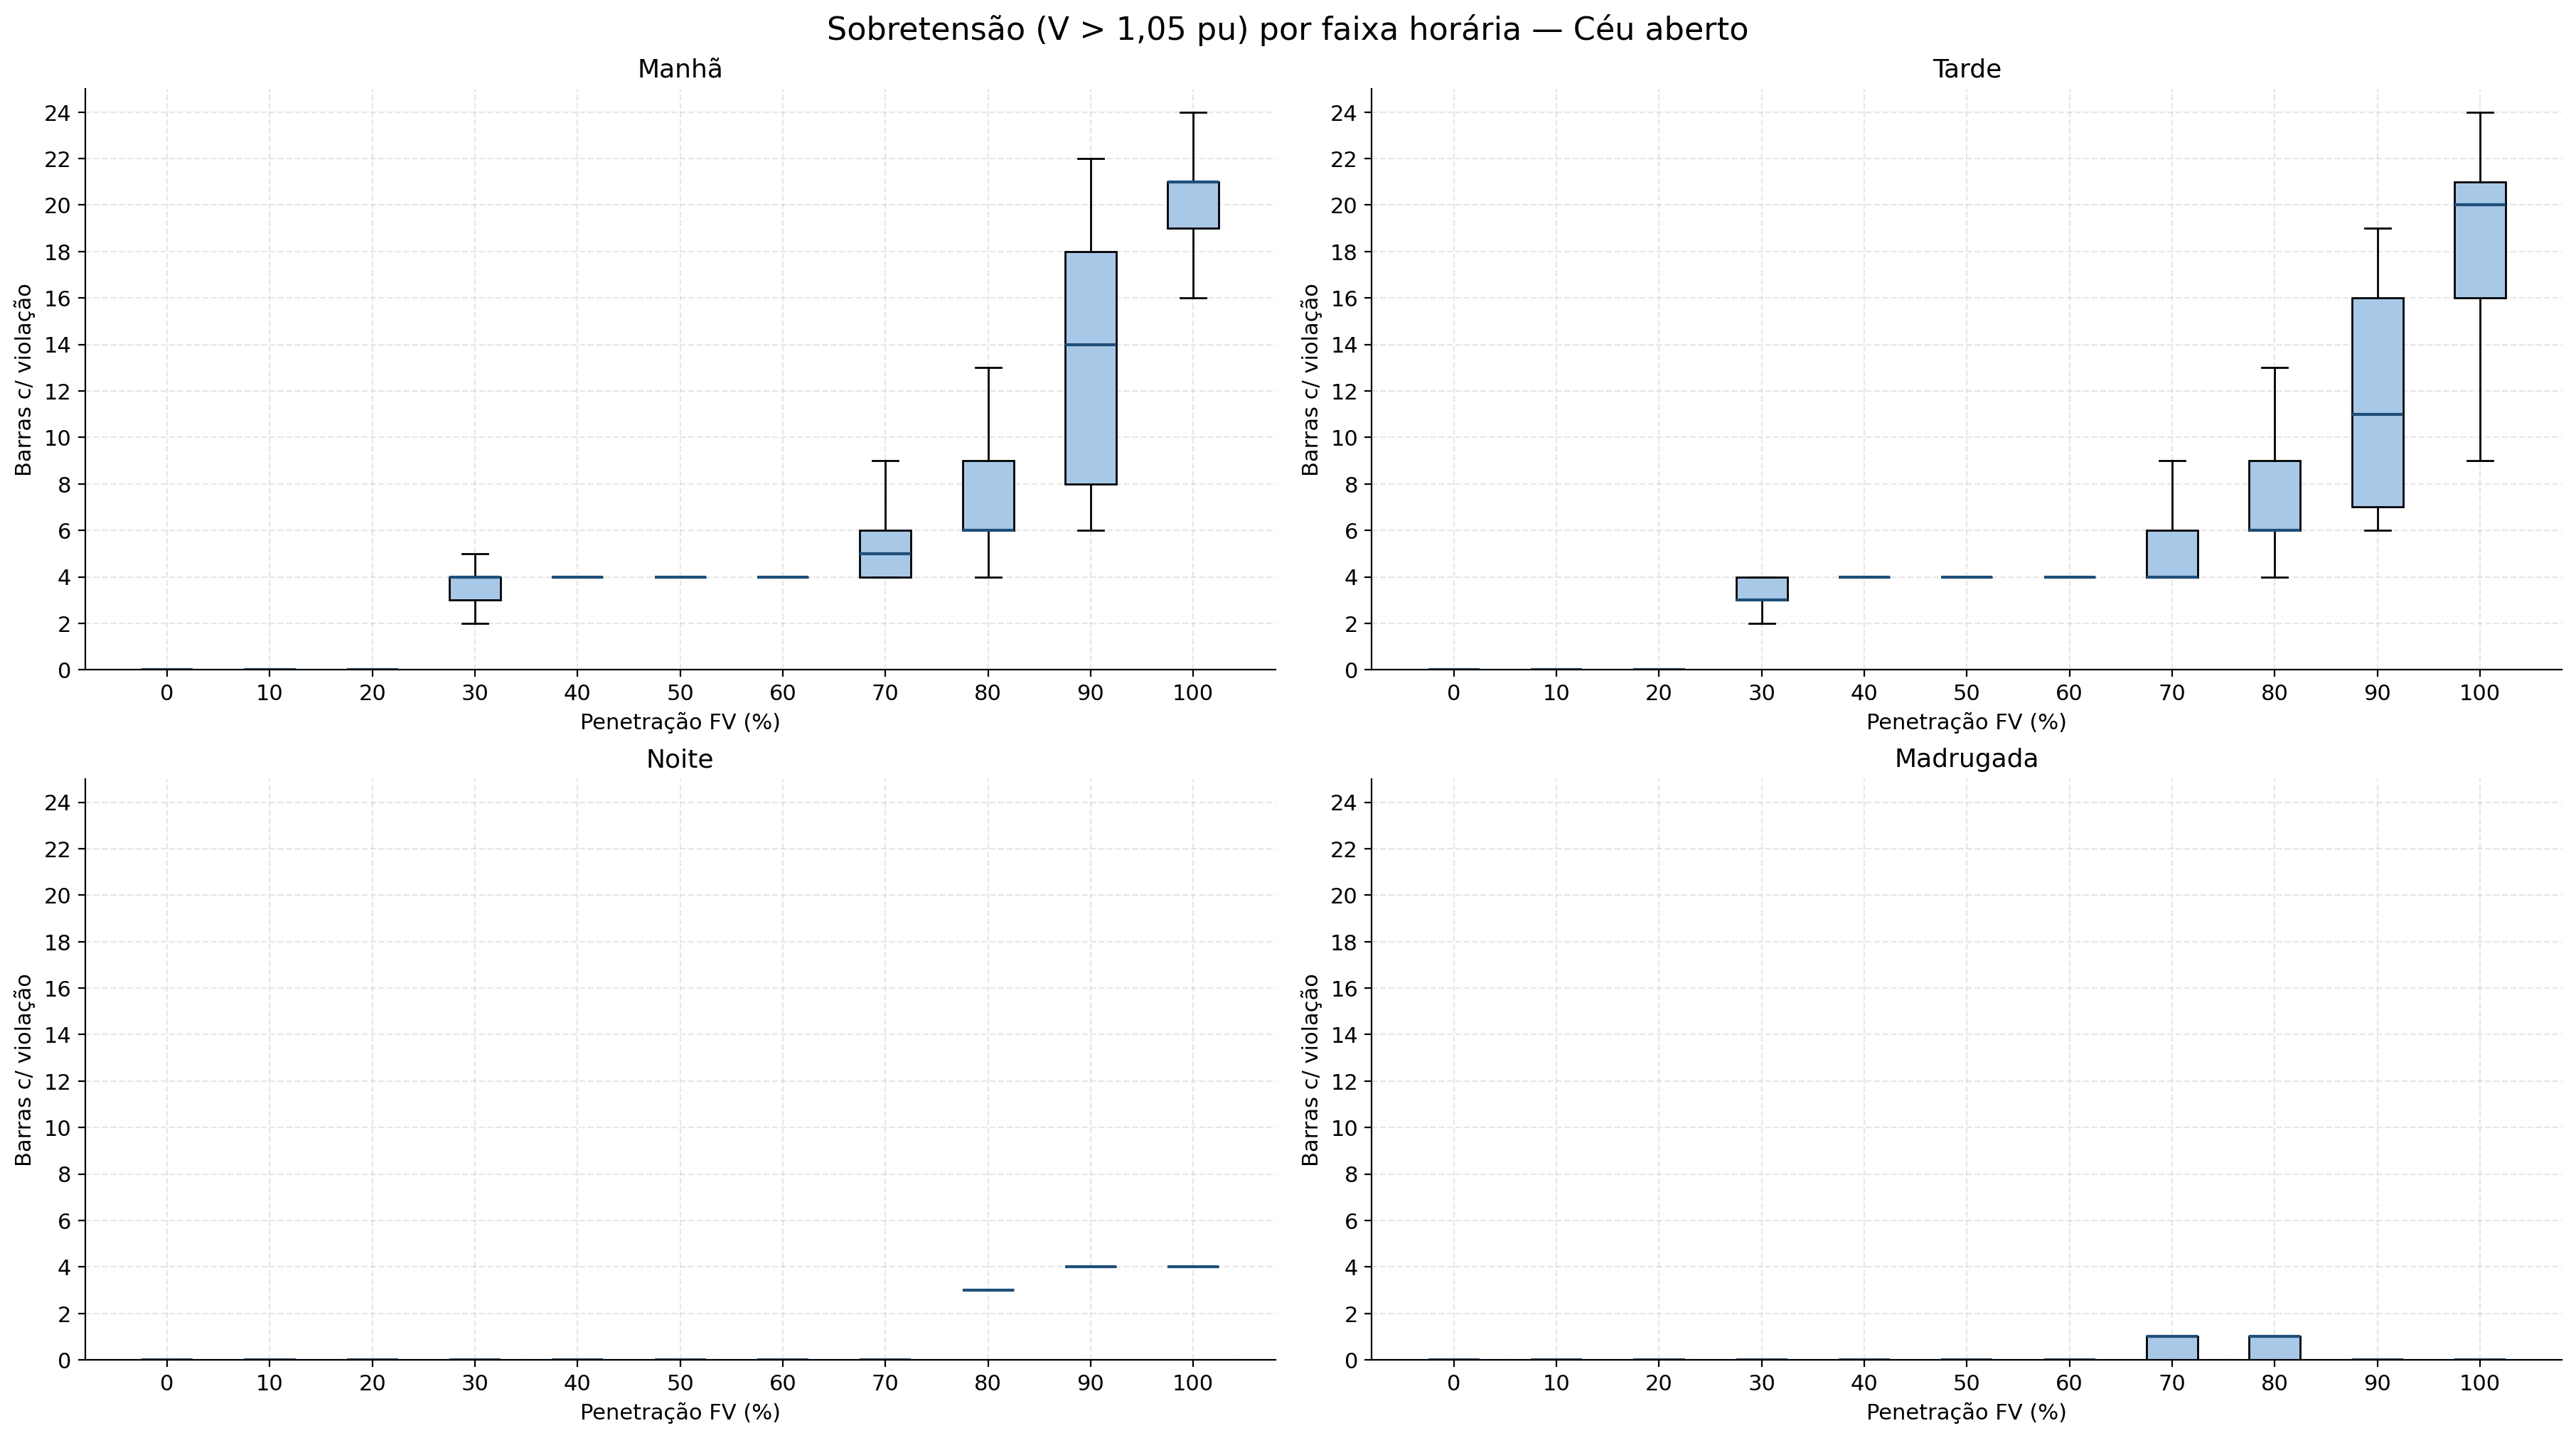
\includegraphics[width=0.92\textwidth]{an_boxplot_sobre_ceuaberto.png}
  \par\vspace{2pt}\fonte{autoria própria}
\end{figure}

\begin{figure}[!htb]
  \centering
  \caption{Número de barras com sobretensão por faixa horária no caso sem controle --- dias nublados.}
  \label{fig:an_box_sobre_nublado}
  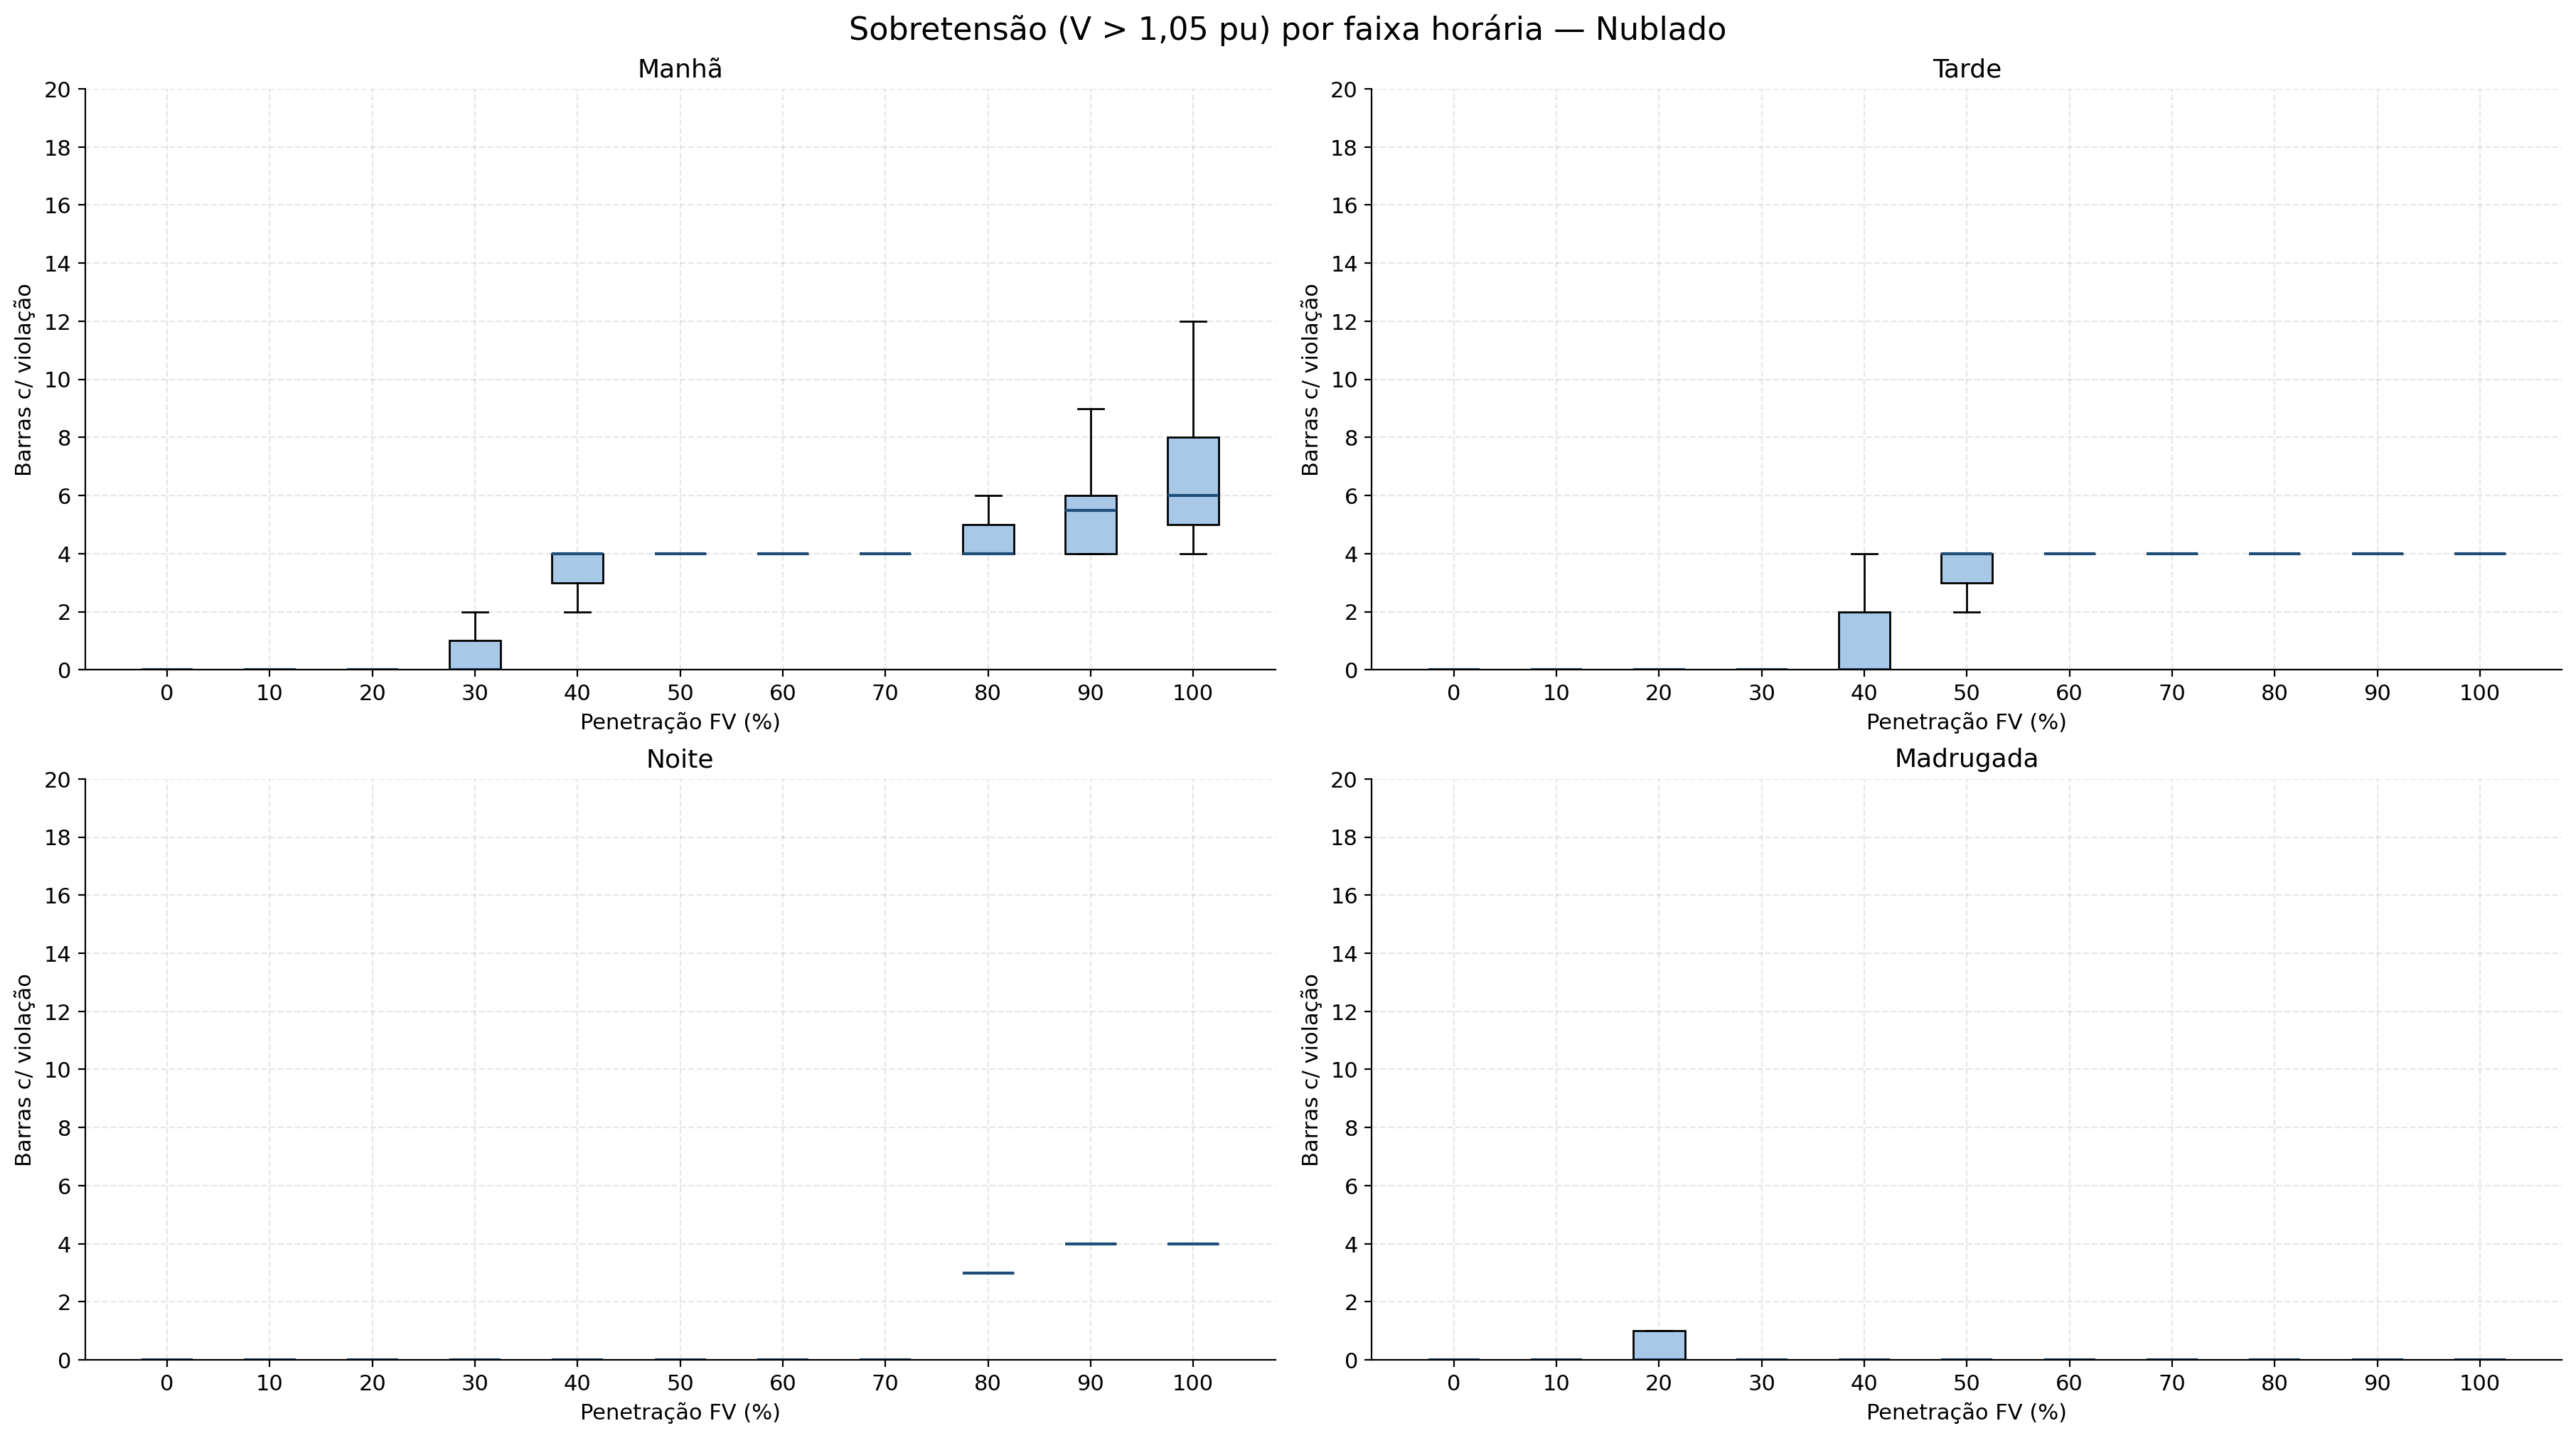
\includegraphics[width=0.92\textwidth]{an_boxplot_sobre_nublado.png}
  \par\vspace{2pt}\fonte{autoria própria}
\end{figure}


\end{document}
